\documentclass{scrreprt}

\usepackage{fontspec}
\usepackage[vietnamese,english]{babel}

\usepackage{listings}
\usepackage{underscore}
\usepackage{graphicx}
\usepackage[bookmarks=true]{hyperref}
\usepackage{float}
\usepackage{enumitem}
\setlist[itemize]{topsep=4pt, itemsep=4pt, parsep=0pt, partopsep=0pt}
\usepackage{pdflscape}
\usepackage{array}
\usepackage{longtable}
\usepackage{tabularray}

\UseTblrLibrary{booktabs}
\DefTblrTemplate{firsthead,middlehead,lasthead}{default}{}

\DefTblrTemplate{firstfoot}{default}{
  \UseTblrTemplate{caption}{default}
}

\DefTblrTemplate{middlefoot}{default}{
  \UseTblrTemplate{capcont}{default}
}

\DefTblrTemplate{lastfoot}{default}{
  \UseTblrTemplate{caption}{default}
}

\usepackage[
    a4paper,
    left=2cm,
    right=2cm,
    top=3cm,
    bottom=3cm
]{geometry}


\hypersetup{
    bookmarks=false,    % show bookmarks bar?
    pdftitle={Software Requirement Specification},    % title
    pdfauthor={Vo An Khoi},                     % author
    pdfsubject={SRS for Community Social Network LKForum},
    pdfkeywords={Website, SRS, Social Media},
    colorlinks=true,       % false: boxed links; true: colored links
    linkcolor=blue,       % color of internal links
    citecolor=black,       % color of links to bibliography
    filecolor=black,        % color of file links
    urlcolor=purple,        % color of external links
    linktoc=page            % only page is linked
}%
\newcounter{appendixmsgcode}
\newcounter{appendixerrcode}
\newcommand{\msgid}[1]{%
  \refstepcounter{appendixmsgcode}%
  MSG-\theappendixmsgcode\label{msg:#1}%
}
\newcommand{\errid}[1]{%
  \refstepcounter{appendixerrcode}%
  ERR-\theappendixerrcode\label{err:#1}%
}
\newcommand{\msgref}[1]{MSG-\ref{msg:#1}}
\newcommand{\errref}[1]{ERR-\ref{err:#1}}
\def\myversion{1.0 }
\date{}
%\title{%

%}
\usepackage{hyperref}
\begin{document}

\begin{flushright}
	\rule{16cm}{5pt}\vskip1cm
	\begin{bfseries}
		\Huge{SOFTWARE REQUIREMENT \\ SPECIFICATION}\\
		\vspace{1.5cm}
		for\\
		\vspace{1.5cm}
		LKFORUM WEBSITE\\
		\vspace{1.5cm}
		\LARGE{Version \myversion}\\
		\vspace{1.5cm}
		Prepared by : Vo An Khoi (23520790)\\
		\vspace{1.5cm}
		Submitted to : Nguyen Trinh Đong \\Lecturer\\
		\vspace{1.5cm}
		May 3, 2026\\
	\end{bfseries}
\end{flushright}

\tableofcontents

\chapter{Introduction}

\section{Purpose}
This SRS describes the functional and nonfunctional requirements for software release 1.0 of the Community Social Network Website (LKForum). This document is intended to be used by the members of the project team who will implement and verify the correct functioning of the system. Unless otherwise noted, all requirements specified here are committed for release 1.0

\section{Intended Audience and Reading Suggestions}
This SRS is for developers, project managers, users and testers. Further the discussion will provide all the internal, external, functional and also non-functional informations about "LKFORUM WEBSITE".

\section{Project Scope}
This SRS describes the functional and nonfunctional requirements for software release 1.0 of the Community Social Network Website (LKForum). This document is intended to be used by the members of the project team who will implement and verify the correct functioning of the system. Unless otherwise noted, all requirements specified here are committed for release 1.0

\section{References}

\begin{itemize}
	\item IEEE Computer Society, \textit{IEEE Recommended Practice for Software Requirements Specifications}, IEEE Std 830-1998.
	
	\item Bass, L., Clements, P., and Kazman, R., \textit{Software Architecture in Practice}, 3rd ed., SEI Series in Software Engineering, Addison-Wesley Professional, 2012.
	
	\item LKForum Project Team, \textit{LKForum Business Requirement Document}, Version 1.0.
\end{itemize}
\chapter{Overall Description}

\section{Product Perspective}
Community Social Network LKForum is a new website that provides a comprehensive, modern solution for building and managing online communities. The context diagram in Figure 1 illustrates the external entities and system interfaces for release 1.0. The system is expected to evolve over several releases, ultimately connecting to third-party social media APIs for authentication (Google, Facebook) and expanding to include advanced content monetization tools and mobile-native applications.

\begin{figure}[H]
    \centering
    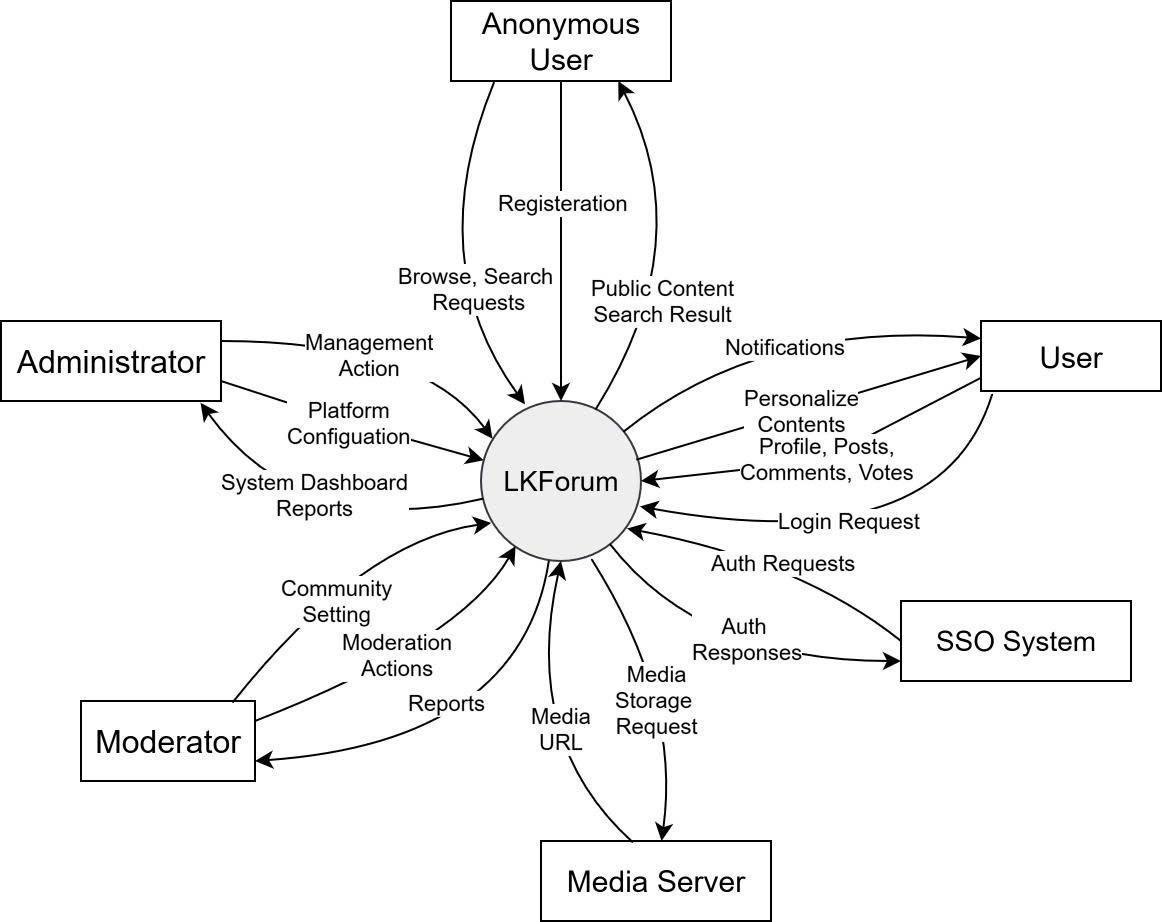
\includegraphics[width=0.8\textwidth]{./diagrams/Context Diagram.jpg}
    \caption{Context diagram for release 1.0 of LKForum}
    \label{fig:context_diagram}
\end{figure}

\section{Operating Environment}

\begin{itemize}[leftmargin=2cm]
    \item[\textbf{OE-1:}] LKForum must operate correctly on modern web browsers including: Google Chrome (latest version), Mozilla Firefox (latest version), Apple Safari (latest version), and Microsoft Edge (latest version).

    \item[\textbf{OE-2:}] Users can access LKForum via the Internet from desktop computers, laptops, and tablets. The interface must have responsive design to be compatible with various screen sizes.
\end{itemize}

\section{Design and Implementation Constraints}

\begin{itemize}[leftmargin=2cm]
    \item[\textbf{CO-1:}] The user interface (front-end) source code must be developed using the Svelte framework.

    \item[\textbf{CO-2:}] The system must use a standard MongoDB NoSQL database with a back-end developed using the Go framework.

    \item[\textbf{CO-3:}] All HTML code must adhere to the HTML 5.0 standard.
\end{itemize}

\section{Assumptions and Dependencies}

\begin{itemize}[leftmargin=2cm]
    \item[\textbf{AS-1:}] It is assumed that users have a stable Internet connection to access and use the platform's features.

    \item[\textbf{DE-1:}] The social media login feature (Google, Facebook) depends on the APIs and policies of these third-party service providers. Any changes on their part may affect the operation of this feature.
\end{itemize}

\chapter{System Features}

The LKForum website is being built using the Go programming language for the back-end, Svelte with Vite for the front-end, MongoDB for primary data storage, and Redis for caching and session management.
\newline
Back-End -- Go with the Gin web framework.
\newline
Front-End -- Svelte with Vite.
\newline
Database -- MongoDB.
\newline
Cache and Session Store -- Redis.

\section{Use Case Description}

\subsection{UC-01 - Sign Up}
\begin{table}[H]
\centering
\begin{tblr}{
    width=\textwidth,
    hlines,
    vlines,
    rows = {valign=m},
    colspec = {Q[l,3cm] Q[l,11cm]}
}
\textbf{Name} & Sign Up \\
\textbf{Description} & This use case describes how a new user creates an account and verifies the email address using OTP. \\
\textbf{Actor} & User \\
\textbf{Trigger} & When the user clicks the ``Sign Up'' button. \\
\textbf{Pre-condition} & The user is not logged in to the system. \newline The user is on the sign up page. \\
\textbf{Post-condition} & The user account is created and verified. \newline The user is authenticated and can access the system. \\
\end{tblr}
\caption{Use Case Specification - Sign Up}
\end{table}

\begin{figure}[H]
	\centering
	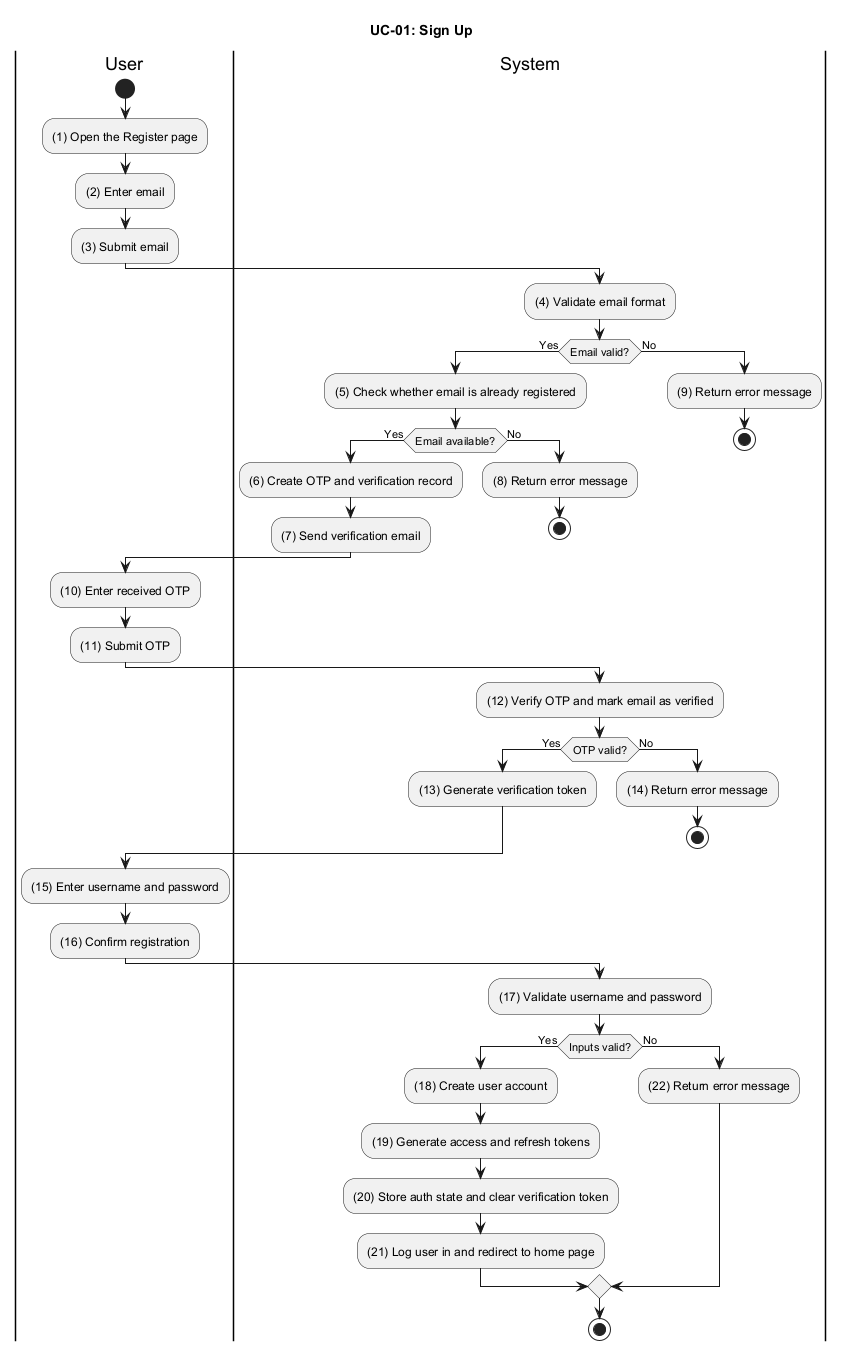
\includegraphics[width=0.8\textwidth]{./diagrams/activity_diagrams/UC_01_Sign_Up.png}
	\caption{Activity Diagram for UC-01 Sign Up}
	\label{fig:ad_uc01}
\end{figure}

\begin{longtblr}[
	caption = {Business Rules for UC-01 - Sign Up},
	label = {tab:uc01_business_rules}
	]{
		width=\textwidth,
		hlines,
		vlines,
		rowhead = 1,
		rows = {valign=m, cmd=\nopagebreak},
		row{1} = {font=\bfseries, halign=c},
		colspec = {Q[c,1.8cm] Q[c,1.5cm] Q[c,3.0cm] Q[l,7.5cm]}
	}
	\textbf{ID} & \textbf{Activity} & \textbf{Rule Type} & \textbf{Description} \\
	
	BR-UC01-01 & (4) & Validation Rules &
	\textbf{Validate Email Format:}
	\begin{itemize}
		\item The system checks that \textbf{email} is present and valid.
		\item If the \textbf{email} is missing or invalid, the system returns a bad-request error.
	\end{itemize} \\
	
	BR-UC01-02 & (5) & Constraint Rules &
	\textbf{Check Email Availability and Prepare Verification Record:}
	\begin{itemize}
		\item The system checks whether the \textbf{email} already exists in the user repository.
		\item If the \textbf{email} already exists, the system returns an email-exists error.
	\end{itemize} \\
	
	BR-UC01-03 & (7) & Message Rules &
	\textbf{Send Verification Email:}
	\begin{itemize}
		\item Successful verification-code delivery shall use \msgref{verification-code-sent} or \msgref{otp-sent-vi}; resending shall use \msgref{new-verification-code-sent} or \msgref{otp-resent-vi}.
		\item OTP validation failures shall return \errref{invalid-otp} or \errref{otp-expired}.
		\item Completed verification and registration shall use \msgref{email-verified-successfully} or \msgref{register-success-vi}; invalid registration data shall return \errref{email-exists}, \errref{invalid-username}, \errref{password-too-short}, or \errref{password-too-weak}.
	\end{itemize} \\
	
	BR-UC01-04 & (12) & Validation Rules &
	\textbf{Verify OTP and Issue Token:}
	\begin{itemize}
		\item The system checks that \textbf{email} and \textbf{otp} are present.
		\item If no verification record exists, the system returns an invalid \textbf{OTP} error.
		\item If the verification record is already marked verified, the system returns an email-already-verified error.
		\item If the \textbf{OTP} does not match or has expired, the system returns an invalid or expired \textbf{OTP} error.
		\item Otherwise, the system marks the verification record as verified and generates a verification token from the verified \textbf{email} and \textbf{nonce}.
	\end{itemize} \\
	
	BR-UC01-05 & (17) & Validation Rules &
	\textbf{Validate Registration Fields:}
	\begin{itemize}
		\item The system checks that \textbf{username} is between 3 and 20 characters.
		\item The system checks that \textbf{password} is at least 8 characters long and strong enough.
	\end{itemize} \\
	
	BR-UC01-06 & (18--20) & Workflow Rules &
	\textbf{Create Account and Complete Login:}
	\begin{itemize}
		\item The system hashes the \textbf{password} with \textbf{\textit{GenerateFromPassword()}} before storing it.
		\item The system checks that the \textbf{username} is still available and that the \textbf{email} is still not registered.
		\item The system creates the new local user with default settings, deletes the verification record, invalidates the \textbf{username} cache, and generates access and refresh tokens using \textbf{\textit{GenerateToken()}}.
	\end{itemize} \\
	
	BR-UC01-07 & (21) & Redirect Rules &
	\textbf{Redirect After Registration:}
	\begin{itemize}
		\item The system logs the user in and redirects to the home page.
	\end{itemize} \\
\end{longtblr}


\subsection{UC-02 - Sign In}
\begin{table}[H]
\centering
\begin{tblr}{
    width=\textwidth,
    hlines,
    vlines,
    rows = {valign=m},
    colspec = {Q[l,3cm] Q[l,11cm]}
}
\textbf{Name} & Sign In \\
\textbf{Description} & This use case describes how a registered user logs into the system using local credentials or Google OAuth. \\
\textbf{Actor} & User \\
\textbf{Trigger} & When the user clicks the ``Sign In'' button. \\
\textbf{Pre-condition} & The user is not logged in to the system. \newline The user is on the sign in page. \\
\textbf{Post-condition} & The user is authenticated. \newline The user is redirected to the appropriate page. \\
\end{tblr}
\caption{Use Case Specification - Sign In}
\end{table}

\begin{figure}[H]
	\centering
	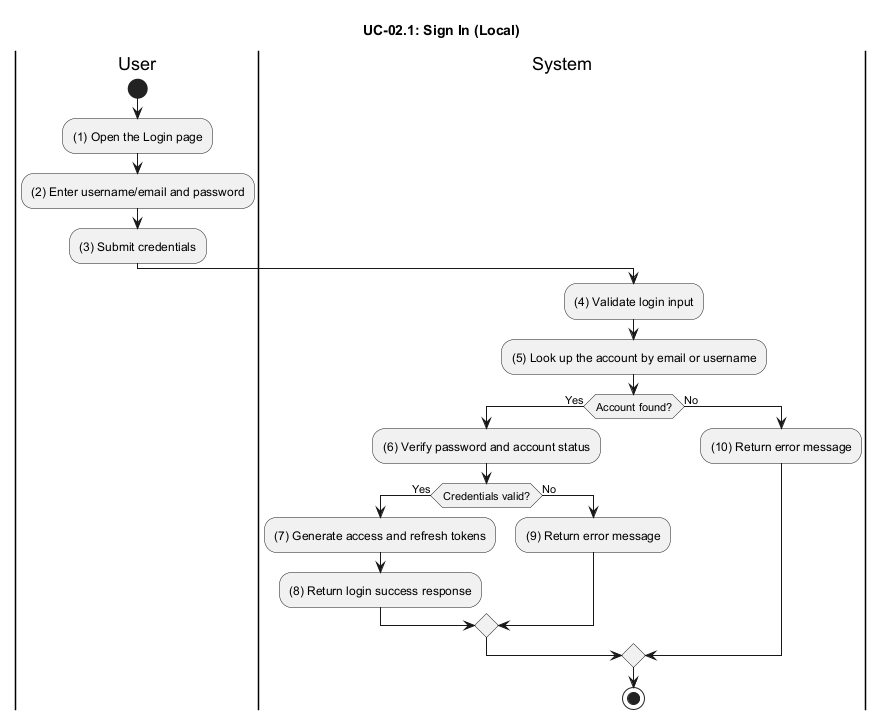
\includegraphics[width=0.8\textwidth]{./diagrams/activity_diagrams/UC_02_Local_Sign_In.png}
	\caption{Activity Diagram for UC-02 Local Sign In}
	\label{fig:ad_uc02_local}
\end{figure}


\begin{longtblr}[
	caption = {Business Rules for UC-02.1 - Sign In (Local)},
	label = {tab:uc02_local_business_rules}
	]{
		width=\textwidth,
		hlines,
		vlines,
		rowhead = 1,
		rows = {valign=m, cmd=\nopagebreak},
		row{1} = {font=\bfseries, halign=c},
		colspec = {Q[c,1.8cm] Q[c,1.5cm] Q[c,3.0cm] Q[l,7.5cm]}
	}
	\textbf{ID} & \textbf{Activity} & \textbf{Rule Type} & \textbf{Description} \\
	
	BR-UC02-01 & (4) & Validation Rules &
	\textbf{Validate Login Input:}
	\begin{itemize}
		\item The controller checks the JSON body for \textbf{identifier} and \textbf{password} in \texttt{UserLoginRequest}.
		\item If binding fails or either field is missing, the controller returns a bad request response.
		\item The controller does not validate the \textbf{identifier} format here; the service decides whether to search by email or username.
	\end{itemize} \\
	
	BR-UC02-02 & (5) & Workflow Rules &
	\textbf{Look Up Account:}
	\begin{itemize}
		\item The service checks whether \textbf{identifier} is an email using \textbf{\textit{isEmail()}}.
		\item The service looks up the account by email or username using the user repository.
		\item If no account exists, the service returns an invalid credentials error.
	\end{itemize} \\
	
	BR-UC02-03 & (6) & Authorization Rules &
	\textbf{Verify Password and Account Status:}
	\begin{itemize}
		\item The system checks that the account uses the local provider.
		\item The service compares the stored password with \textbf{password} using \textbf{\textit{bcrypt.CompareHashAndPassword()}}.
		\item If the password hash is empty or the comparison fails, the service returns an invalid credentials error.
		\item If \textbf{IsVerified} is false, the service returns an email-not-verified error.
		\item If the user is banned and the ban has not expired, the service returns a user-inactive error.
	\end{itemize} \\
	
	BR-UC02-04 & (7--10) & Message Rules &
	\textbf{Return Authentication Response:}
	\begin{itemize}
		\item Successful local sign-in shall use \msgref{login-successful}.
		\item Failed local sign-in shall return \errref{invalid-credentials}.
		\item Google sign-in and setup failures shall return \errref{invalid-token}, \errref{login-method-mismatch}, or \errref{email-exists} as applicable.
	\end{itemize} \\
\end{longtblr}


\begin{figure}[H]
    \centering
    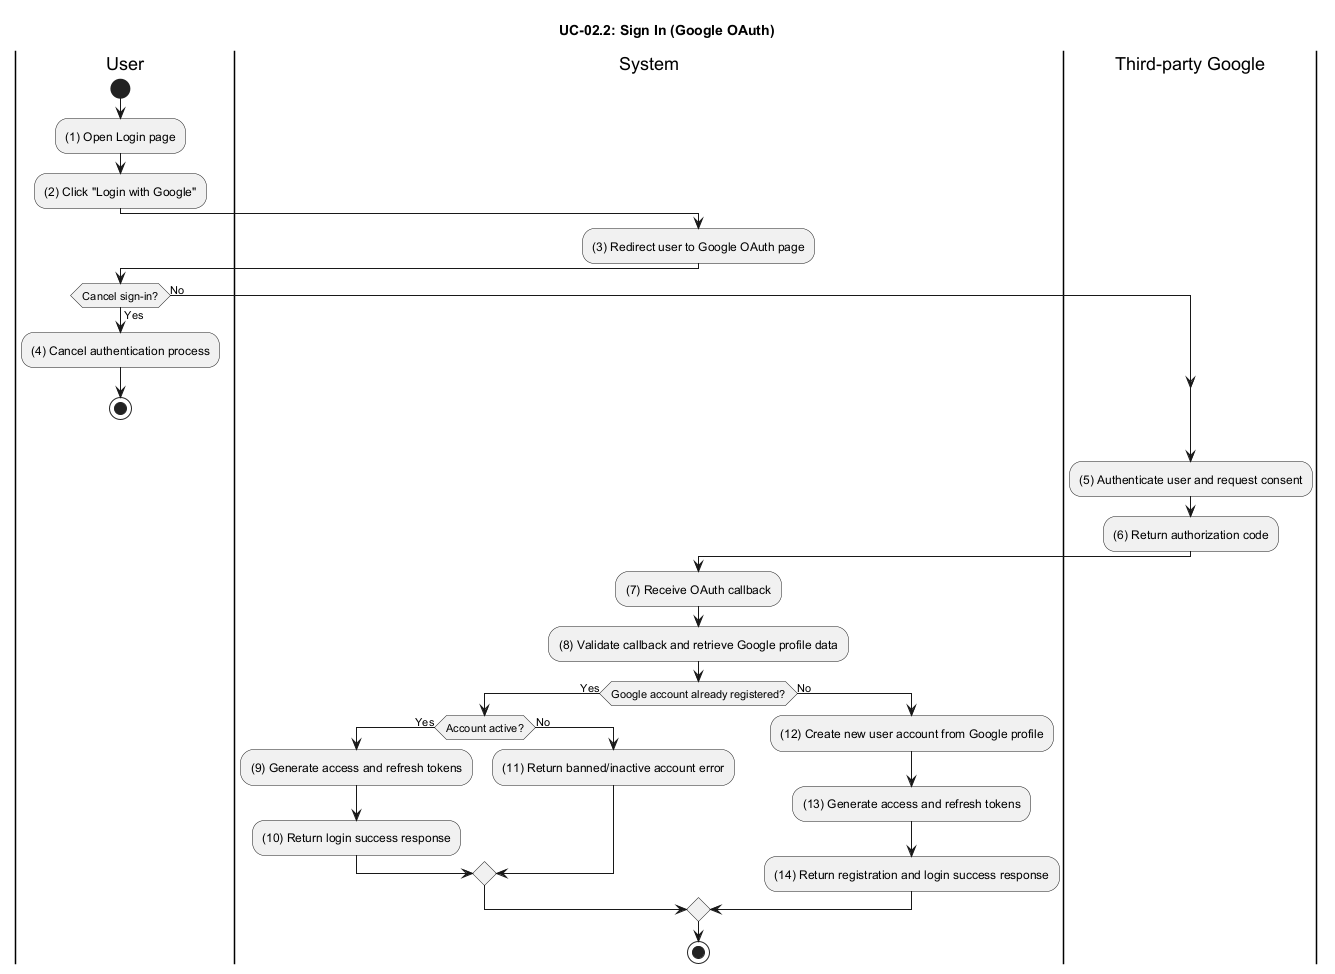
\includegraphics[width=\textwidth]{./diagrams/activity_diagrams/UC_02_Google_Sign_In.png}
    \caption{Activity Diagram for UC-02 Google Sign In}
    \label{fig:ad_uc02_google}
\end{figure}

\begin{longtblr}[
	caption = {Business Rules for UC-02.2 - Sign In (Google OAuth)},
	label = {tab:uc02_google_business_rules}
	]{
		width=\textwidth,
		hlines,
		vlines,
		rowhead = 1,
		rows = {valign=m, cmd=\nopagebreak},
		row{1} = {font=\bfseries, halign=c},
		colspec = {Q[c,1.8cm] Q[c,1.5cm] Q[c,3.0cm] Q[l,7.5cm]}
	}
	\textbf{ID} & \textbf{Activity} & \textbf{Rule Type} & \textbf{Description} \\
	
	BR-UC02-05 & (3) & Redirect Rules &
	\textbf{Start Google OAuth Flow:}
	\begin{itemize}
		\item The system redirects the user to Google OAuth using a generated state value.
		\item Google authenticates the user and returns an authorization code.
	\end{itemize} \\
	
	BR-UC02-06 & (8) & Validation Rules &
	\textbf{Process Google Callback:}
	\begin{itemize}
		\item The controller checks that the callback contains \textbf{code}.
		\item If \textbf{code} is missing, the controller redirects to the frontend error page with a missing-auth-code message.
		\item The service exchanges \textbf{code} for Google profile data using \textbf{\textit{GetGoogleUserInfo()}}.
		\item If Google rejects the authorization code or profile lookup fails, the controller redirects to the frontend error page with the returned error message.
	\end{itemize} \\
	
	BR-UC02-07 & (9--11) & Authorization Rules &
	\textbf{Login or Setup Decision:}
	\begin{itemize}
		\item If an account exists and \textbf{provider} is Google, the service generates access and refresh tokens using \textbf{\textit{GenerateToken()}}.
		\item If the account belongs to a different login method, the service returns a login-method-mismatch error.
		\item If the account is banned and the ban has not expired, the service returns a user-inactive error.
		\item If no Google account exists, the service creates a setup token using \textbf{\textit{CreateSetupToken()}} and returns the setup-required result.
	\end{itemize} \\
	
	BR-UC02-08 & (12) & Validation Rules &
	\textbf{Validate Google Setup Input:}
	\begin{itemize}
		\item The controller checks the JSON body for \textbf{setup\_token} and \textbf{username} in \texttt{CompleteGoogleSetupRequest}.
		\item If binding fails or \textbf{setup\_token} is missing, the controller returns a bad request response.
		\item The service validates that \textbf{username} is at least 3 characters and no more than 20 characters.
		\item If \textbf{username} already exists, the service returns a username-exists error.
		\item If the Google email is already taken, the service returns an email-exists error.
	\end{itemize} \\
	
	BR-UC02-09 & (13) & Workflow Rules &
	\textbf{Create Google Account:}
	\begin{itemize}
		\item The system parses \textbf{setup\_token} to recover the Google claims.
		\item The system creates the user with \textbf{provider} set to Google, stores \textbf{provider\_id}, applies default settings, and copies the Google avatar URL when available.
		\item The system generates access and refresh tokens after the user is created.
	\end{itemize} \\
	
	BR-UC02-10 & (14) & Message Rules &
	\textbf{Return Setup Success:}
	\begin{itemize}
		\item Successful Google-account completion shall use \msgref{login-successful} after the account and tokens are issued.
		\item Validation failures during setup shall return \errref{email-exists}, \errref{invalid-username}, \errref{password-too-short}, or \errref{password-too-weak} when relevant.
	\end{itemize} \\
\end{longtblr}



\subsection{UC-03 - Forgot Password}
\begin{table}[H]
\centering
\begin{tblr}{
    width=\textwidth,
    hlines,
    vlines,
    rows = {valign=m},
    colspec = {Q[l,3cm] Q[l,11cm]}
}
\textbf{Name} & Forgot Password \\
\textbf{Description} & This use case describes how a user resets a forgotten password through email verification and OTP. \\
\textbf{Actor} & User \\
\textbf{Trigger} & When the user clicks the ``Forgot Password'' link. \\
\textbf{Pre-condition} & The user has an existing account and can access the registered email address. \newline The user is not logged in to the system. \\
\textbf{Post-condition} & The user password is reset successfully. \newline The user can sign in again with the new password. \\
\end{tblr}
\caption{Use Case Specification - Forgot Password}
\end{table}


\begin{figure}[H]
    \centering
    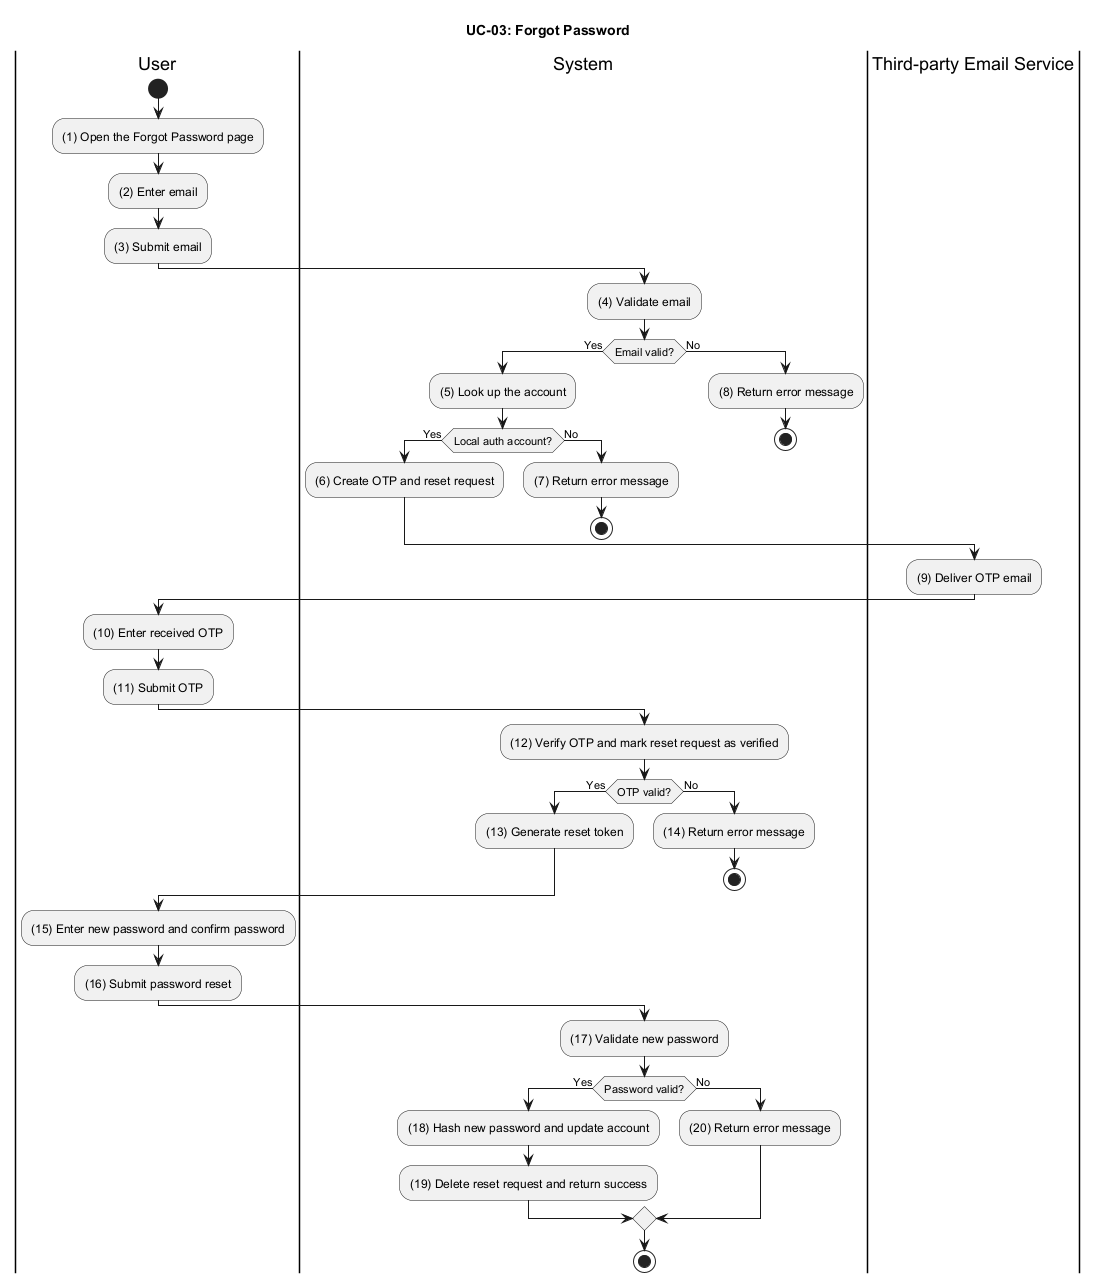
\includegraphics[width=0.7\textwidth]{./diagrams/activity_diagrams/UC_03_Forgot_Password.png}
    \caption{Activity Diagram for UC-03}
    \label{fig:ad_uc03}
\end{figure}


\begin{longtblr}[
	caption = {Business Rules for UC-03 - Forgot Password},
	label = {tab:uc03_business_rules}
	]{
		width=\textwidth,
		hlines,
		vlines,
		rowhead = 1,
		rows = {valign=m, cmd=\nopagebreak},
		row{1} = {font=\bfseries, halign=c},
		colspec = {Q[c,1.8cm] Q[c,1.5cm] Q[c,3.0cm] Q[l,7.5cm]}
	}
	\textbf{ID} & \textbf{Activity} & \textbf{Rule Type} & \textbf{Description} \\
	
	BR-UC03-01 & (4) & Validation Rules &
	\textbf{Validate Reset Request:}
	\begin{itemize}
		\item The controller checks \textbf{email} in \texttt{ForgotPasswordRequest}.
		\item If binding fails or \textbf{email} is missing or invalid, the controller returns a bad request response.
	\end{itemize} \\
	
	BR-UC03-02 & (5) & Authorization Rules &
	\textbf{Validate Account Ownership:}
	\begin{itemize}
		\item The service looks up the account by \textbf{email} using the user repository.
		\item If the account does not exist, the service returns an email-not-registered error.
		\item If the account exists but the \textbf{provider} is not local, the service returns a login-method-mismatch error.
	\end{itemize} \\
	
	BR-UC03-03 & (6) & Workflow Rules &
	\textbf{Create Password Reset Request:}
	\begin{itemize}
		\item The system deletes any existing reset record for the same \textbf{email}.
		\item The system generates a 6-digit \textbf{OTP}, a \textbf{nonce}, and an expiry timestamp using \textbf{\textit{generateOTP()}} and \textbf{\textit{generateNonce()}}.
		\item The system stores a new password-reset record with \textbf{IsVerified = false}.
	\end{itemize} \\
	
	BR-UC03-04 & (7) & Message Rules &
	\textbf{Return Reset Request Result:}
	\begin{itemize}
		\item Successful reset-code delivery shall use \msgref{password-reset-code-sent}.
		\item If the account is not local, the service shall return \errref{login-method-mismatch}; unknown local accounts shall return \errref{email-not-registered}.
	\end{itemize} \\
	
	BR-UC03-05 & (12) & Validation Rules &
	\textbf{Validate Reset OTP:}
	\begin{itemize}
		\item The controller checks \textbf{email} and \textbf{otp} in \texttt{VerifyResetPasswordOTPRequest}.
		\item If binding fails, the controller returns a bad request response.
		\item If no reset record exists for the \textbf{email}, the service returns an invalid \textbf{OTP} error.
		\item If the reset record is already verified, the service returns an email-already-verified error.
		\item If the \textbf{OTP} does not match or has expired, the service returns an invalid or expired \textbf{OTP} error.
	\end{itemize} \\
	
	BR-UC03-06 & (12) & Workflow Rules &
	\textbf{Verify OTP and Generate Reset Token:}
	\begin{itemize}
		\item The service marks the reset record as verified.
		\item The service generates a reset token from the verified \textbf{email} and \textbf{nonce} using \textbf{\textit{CreateVerificationToken()}}.
	\end{itemize} \\
	
	BR-UC03-07 & (14) & Message Rules &
	\textbf{Return OTP Error:}
	\begin{itemize}
		\item Successful reset-OTP verification shall use \msgref{otp-verified-successfully}.
		\item Invalid or expired reset OTP values shall return \errref{invalid-otp} or \errref{otp-expired}.
	\end{itemize} \\
	
	BR-UC03-08 & (17) & Validation Rules &
	\textbf{Validate New Password:}
	\begin{itemize}
		\item The controller checks \textbf{reset\_token} and \textbf{new\_password} in \texttt{ResetPasswordRequest}.
		\item If binding fails or \textbf{reset\_token} is missing, the controller returns a bad request response.
		\item The DTO binding requires \textbf{new\_password} to be present and at least 6 characters long.
		\item The service requires \textbf{new\_password} to be at least 8 characters long.
		\item The service requires \textbf{new\_password} to contain uppercase, lowercase, numeric, and special characters.
	\end{itemize} \\
	
	BR-UC03-09 & (18) & Workflow Rules &
	\textbf{Hash and Update Password:}
	\begin{itemize}
		\item The service parses the reset token and verifies the stored \textbf{nonce}.
		\item The service looks up the user by \textbf{email}.
		\item The service hashes \textbf{new\_password} with \textbf{\textit{GenerateFromPassword()}}.
		\item The service updates the user password in the repository.
	\end{itemize} \\
	
	BR-UC03-10 & (19) & Workflow Rules &
	\textbf{Clean Up Reset Record:}
	\begin{itemize}
		\item The service deletes the reset record after a successful password change.
		\item The controller returns a success response telling the user they can log in with the new password.
	\end{itemize} \\
	
	BR-UC03-11 & (20) & Message Rules &
	\textbf{Return Password Error:}
	\begin{itemize}
		\item Successful password reset shall use \msgref{password-reset-successfully} or \msgref{change-password-success-vi}.
		\item Invalid replacement passwords shall return \errref{password-too-short} or \errref{password-too-weak}.
	\end{itemize} \\
\end{longtblr}


\subsection{UC-04 - Manage Profile}
\begin{table}[H]
\centering
\begin{tblr}{
    width=\textwidth,
    hlines,
    vlines,
    rows = {valign=m},
    colspec = {Q[l,3cm] Q[l,11cm]}
}
\textbf{Name} & Manage Profile \\
\textbf{Description} & This use case describes how a user updates profile information such as bio, avatar, and cover image. \\
\textbf{Actor} & User \\
\textbf{Trigger} & When the user opens the profile edit page. \\
\textbf{Pre-condition} & The user is logged in to the system. \newline The user has permission to edit the profile. \\
\textbf{Post-condition} & The profile information is updated and stored. \newline The new profile data is visible across the system. \\
\end{tblr}
\caption{Use Case Specification - Manage Profile}
\end{table}


\begin{figure}[H]
    \centering
    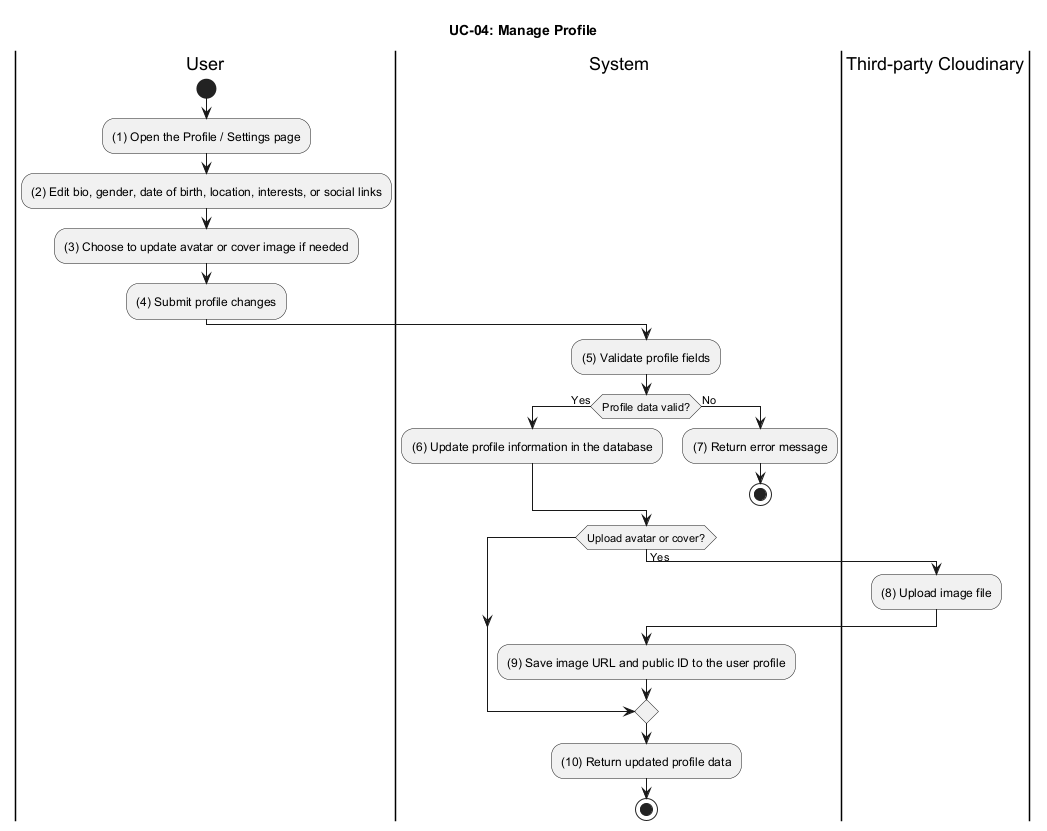
\includegraphics[width=\textwidth]{./diagrams/activity_diagrams/UC_04_Manage_Profile.png}
    \caption{Activity Diagram for UC-04}
    \label{fig:ad_uc04}
\end{figure}

\begin{longtblr}[
    caption = {Business Rules for UC-04 - Manage Profile},
    label = {tab:uc04_business_rules}
]{
    width=\textwidth,
    hlines,
    vlines,
    rowhead = 1,
    rows = {valign=m, cmd=\nopagebreak},
    row{1} = {font=\bfseries, halign=c},
    colspec = {Q[c,1.8cm] Q[c,1.5cm] Q[c,3.0cm] Q[l,7.5cm]}
}
\textbf{ID} & \textbf{Activity} & \textbf{Rule Type} & \textbf{Description} \\

BR-UC04-01 & (5) & Validation Rules &
\textbf{Validate Profile Fields:}
\begin{itemize}
    \item The controller checks the JSON body for \texttt{UserProfileUpdateRequest}.
    \item If binding fails, the controller returns a bad request response.
    \item \textbf{bio} is limited by DTO validation to 500 characters.
    \item \textbf{social\_links.website} must be a valid URL when provided.
\end{itemize} \\

BR-UC04-02 & (6) & Workflow Rules &
\textbf{Update Profile Data:}
\begin{itemize}
    \item The service loads the current user and updates \textbf{RoleContent.AsUser}.
    \item Empty string values clear the corresponding profile field.
    \item The service accepts updates for \textbf{gender}, \textbf{date\_of\_birth}, \textbf{location}, \textbf{interests}, and \textbf{social\_links}.
\end{itemize} \\

BR-UC04-03 & (7) & Validation Rules &
\textbf{Reject Invalid Profile Values:}
\begin{itemize}
    \item If \textbf{gender} is not valid, the service returns an invalid gender error.
    \item If \textbf{date\_of\_birth} cannot be parsed as \texttt{2006-01-02}, the service returns an invalid date format error.
    \item If the calculated age is below 13, the service returns an age-too-young error.
    \item If the calculated age is above 150, the service returns an invalid birth date error.
    \item If \textbf{location} is not a valid province, the service returns an invalid province error.
    \item If more than 10 interests are submitted or any interest is invalid, the service returns an error.
\end{itemize} \\

BR-UC04-04 & (8) & Workflow Rules &
\textbf{Upload Profile Image:}
\begin{itemize}
    \item When the user uploads an avatar or cover image, the controller sends the file to \textbf{\textit{cloudinary.UploadImages()}}.
    \item The service stores the returned image \textbf{URL} and \textbf{PublicID} in the user profile.
    \item If an older image exists, the service deletes the old asset asynchronously using \textbf{\textit{cloudinary.Delete()}}.
\end{itemize} \\

BR-UC04-05 & (9) & Workflow Rules &
\textbf{Save Image Metadata:}
\begin{itemize}
    \item The service updates \textbf{Avatar} or \textbf{Cover} with the new image metadata.
    \item The service persists the updated user profile in the repository.
\end{itemize} \\

BR-UC04-06 & (10) & Message Rules &
\textbf{Return Updated Profile:}
\begin{itemize}
    \item Successful profile and avatar actions shall use \msgref{profile-updated}, \msgref{avatar-upload-success}, \msgref{avatar-delete-success}, and the confirmation prompt \msgref{confirm-delete-avatar}.
    \item Failed profile updates shall use \msgref{profile-update-failed}, \msgref{avatar-upload-failed}, or \msgref{avatar-delete-failed}.
    \item Validation failures shall return \errref{user-not-found}, \errref{invalid-gender}, \errref{invalid-date-format}, \errref{invalid-birth-date}, \errref{invalid-province}, \errref{too-many-interests}, or \errref{invalid-interest}.
\end{itemize} \\
\end{longtblr}


\subsection{UC-05 - Change Settings}
\begin{table}[H]
\centering
\begin{tblr}{
    width=\textwidth,
    hlines,
    vlines,
    rows = {valign=m},
    colspec = {Q[l,3cm] Q[l,11cm]}
}
\textbf{Name} & Change Settings \\
\textbf{Description} & This use case describes how a user changes account preferences such as privacy, notifications, and theme. \\
\textbf{Actor} & User \\
\textbf{Trigger} & When the user opens the settings page. \\
\textbf{Pre-condition} & The user is logged in to the system. \newline The settings page is available to the user. \\
\textbf{Post-condition} & The selected preferences are saved. \newline The account settings are updated for future sessions. \\
\end{tblr}
\caption{Use Case Specification - Change Settings}
\end{table}


\begin{figure}[H]
    \centering
    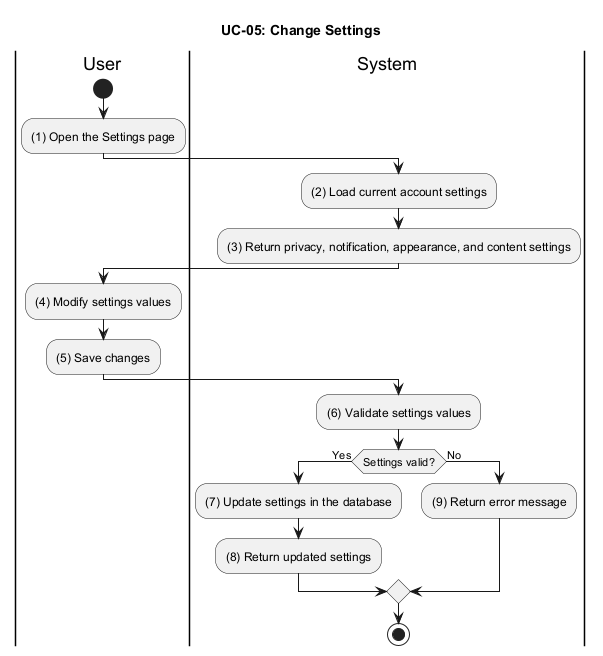
\includegraphics[width=0.8\textwidth]{./diagrams/activity_diagrams/UC_05_Change_Settings.png}
    \caption{Activity Diagram for UC-05}
    \label{fig:ad_uc05}
\end{figure}


\begin{longtblr}[
    caption = {Business Rules for UC-05 - Change Settings},
    label = {tab:uc05_business_rules}
]{
    width=\textwidth,
    hlines,
    vlines,
    rowhead = 1,
    rows = {valign=m, cmd=\nopagebreak},
    row{1} = {font=\bfseries, halign=c},
    colspec = {Q[c,1.8cm] Q[c,1.5cm] Q[c,3.0cm] Q[l,7.5cm]}
}
\textbf{ID} & \textbf{Activity} & \textbf{Rule Type} & \textbf{Description} \\

BR-UC05-01 & (2) & Workflow Rules &
\textbf{Load Current Settings:}
\begin{itemize}
    \item The system loads the current user's settings from the database using \textbf{\textit{GetSettings()}}.
    \item If the user has no settings record, the service returns default settings through \textbf{\textit{FromSettings()}}.
\end{itemize} \\

BR-UC05-02 & (6) & Validation Rules &
\textbf{Validate Settings Values:}
\begin{itemize}
    \item The system checks the JSON body for \texttt{UpdateSettingsRequest}.
    \item If binding fails, the controller returns a bad request response.
    \item \textbf{theme} must be one of \texttt{light}, \texttt{dark}, or \texttt{auto}.
    \item \textbf{font\_size} must be one of \texttt{small}, \texttt{medium}, or \texttt{large}.
\end{itemize} \\

BR-UC05-03 & (7) & Workflow Rules &
\textbf{Update Settings in Database:}
\begin{itemize}
    \item The service loads the current user and initializes \textbf{Settings} when it is nil.
    \item The service updates only the settings fields provided in the request.
    \item The service persists the updated user record using the user repository.
\end{itemize} \\

BR-UC05-04 & (8) & Message Rules &
\textbf{Return Updated Settings:}
\begin{itemize}
    \item Successful account-setting changes shall use \msgref{settings-saved} or \msgref{change-password-success-vi}.
    \item The response includes the updated \textbf{appearance}, \textbf{notifications}, \textbf{privacy}, and \textbf{content} values.
\end{itemize} \\

BR-UC05-05 & (9) & Message Rules &
\textbf{Return Error Message:}
\begin{itemize}
    \item Failed setting updates shall use \msgref{settings-save-failed} or \msgref{password-change-failed}.
    \item Invalid input or authentication failures shall return \errref{bad-request}, \errref{invalid-token}, \errref{not-authenticated}, or \errref{no-fields-to-update}.
\end{itemize} \\
\end{longtblr}


\subsection{UC-06 - View Activity History}
\begin{table}[H]
\centering
\begin{tblr}{
    width=\textwidth,
    hlines,
    vlines,
    rows = {valign=m},
    colspec = {Q[l,3cm] Q[l,11cm]}
}
\textbf{Name} & View Activity History \\
\textbf{Description} & This use case describes how a user reviews past posts, comments, and interactions. \\
\textbf{Actor} & User \\
\textbf{Trigger} & When the user opens the activity history page. \\
\textbf{Pre-condition} & The user is logged in to the system. \newline The user has activity records in the system. \\
\textbf{Post-condition} & The activity history is displayed to the user. \newline The user can review prior activity. \\
\end{tblr}
\caption{Use Case Specification - View Activity History}
\end{table}


\begin{figure}[H]
    \centering
    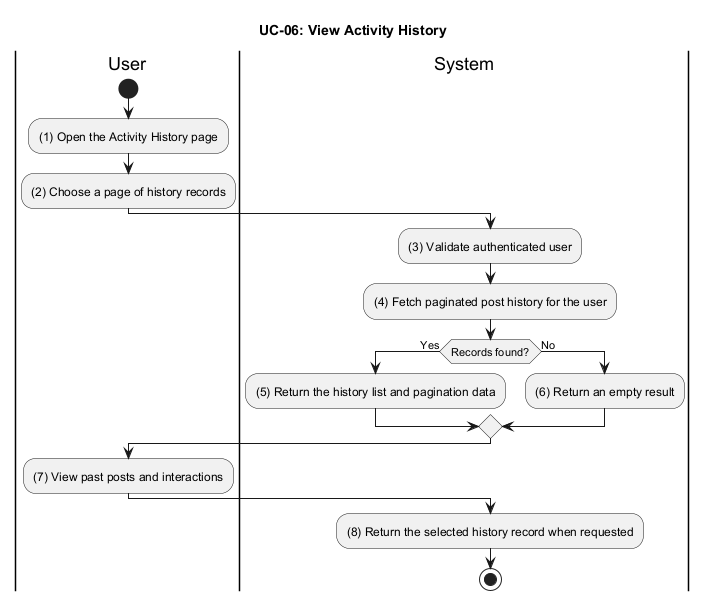
\includegraphics[width=0.9\textwidth]{./diagrams/activity_diagrams/UC_06_View_Activity_History.png}
    \caption{Activity Diagram for UC-06}
    \label{fig:ad_uc06}
\end{figure}

\begin{longtblr}[
    caption = {Business Rules for UC-06 - View Activity History},
    label = {tab:uc06_business_rules}
]{
    width=\textwidth,
    hlines,
    vlines,
    rowhead = 1,
    rows = {valign=m, cmd=\nopagebreak},
    row{1} = {font=\bfseries, halign=c},
    colspec = {Q[c,1.8cm] Q[c,1.5cm] Q[c,3.0cm] Q[l,7.5cm]}
}
\textbf{ID} & \textbf{Activity} & \textbf{Rule Type} & \textbf{Description} \\

BR-UC06-01 & (3) & Authorization Rules &
\textbf{Validate Authenticated User:}
\begin{itemize}
    \item if \textbf{authUser} is missing, then the controller returns a forbidden response.
    \item if \textbf{authUser} exists, then the system continues to fetch the activity history for that user.
\end{itemize} \\

BR-UC06-02 & (4) & Workflow Rules &
\textbf{Fetch Paginated History:}
\begin{itemize}
    \item if \textbf{user\_id} does not match the authenticated user, then the service returns a forbidden error.
    \item if the request is valid, then the service calls \textbf{\textit{GetPostHistoryByUserID()}} to fetch the user's post history.
    \item if \textbf{page} or \textbf{page\_size} is invalid, then the controller uses defaults of 1 and 10.
\end{itemize} \\

BR-UC06-03 & (5--6) & Message Rules &
\textbf{Return History List or Empty Result:}
\begin{itemize}
    \item This use case has no dedicated success toast; successful history retrieval returns the activity list or an empty result directly in the UI.
    \item History-loading failures shall return \errref{not-authenticated}, \errref{forbidden}, \errref{invalid-id}, or \errref{pagination-invalid}.
\end{itemize} \\

BR-UC06-04 & (7) & Authorization Rules &
\textbf{Check Record Ownership:}
\begin{itemize}
    \item if the requester opens a selected history record, then the service checks that \textbf{requesterID} matches the stored \textbf{UserID}.
    \item if the requester does not own the record, then the service returns a forbidden error.
\end{itemize} \\

BR-UC06-05 & (8) & Message Rules &
\textbf{Return Selected History Record:}
\begin{itemize}
    \item This use case has no dedicated success toast; the selected history item is returned inline after conversion with \textbf{\textit{FromPostHistory()}}.
    \item Ownership or lookup failures shall return \errref{forbidden}, \errref{invalid-id}, or \errref{post-not-found}.
\end{itemize} \\
\end{longtblr}


\subsection{UC-07 - Follow / Unfollow User}
\begin{table}[H]
\centering
\begin{tblr}{
    width=\textwidth,
    hlines,
    vlines,
    rows = {valign=m},
    colspec = {Q[l,3cm] Q[l,11cm]}
}
\textbf{Name} & Follow / Unfollow User \\
\textbf{Description} & This use case describes how a user subscribes to or unsubscribes from another user's activity feed. \\
\textbf{Actor} & User \\
\textbf{Trigger} & When the user clicks the follow or unfollow action on another profile. \\
\textbf{Pre-condition} & The user is logged in to the system. \newline The target profile is available for follow actions. \\
\textbf{Post-condition} & The follow relationship is created or removed. \newline The user's feed and follower lists are updated. \\
\end{tblr}
\caption{Use Case Specification - Follow / Unfollow User}
\end{table}


\begin{figure}[H]
    \centering
    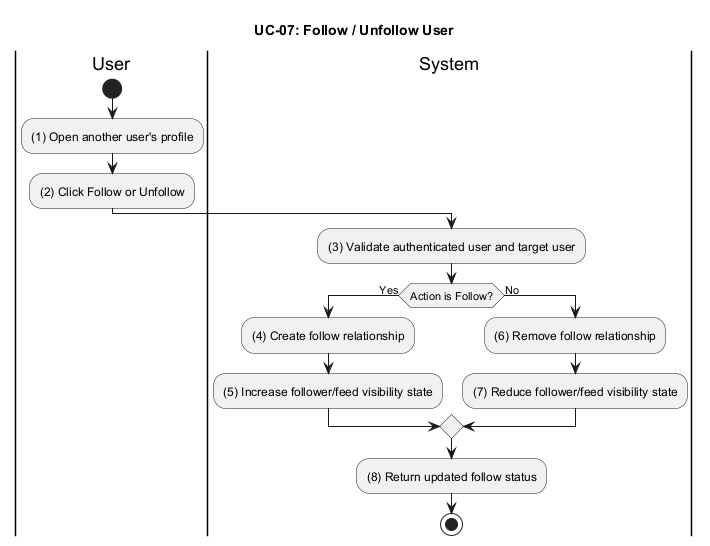
\includegraphics[width=\textwidth]{./diagrams/activity_diagrams/UC_07_Follow_Unfollow_User.png}
    \caption{Activity Diagram for UC-07}
    \label{fig:ad_uc07}
\end{figure}

\begin{longtblr}[
    caption = {Business Rules for UC-07 - Follow / Unfollow User},
    label = {tab:uc07_business_rules}
]{
    width=\textwidth,
    hlines,
    vlines,
    rowhead = 1,
    rows = {valign=m, cmd=\nopagebreak},
    row{1} = {font=\bfseries, halign=c},
    colspec = {
        Q[c,1.5cm]
        Q[c,1.5cm]
        Q[l,11cm]
    }
}
\textbf{Activity} & \textbf{BR Code} & \textbf{Description} \\

(3--6) & BR1 &
\textbf{Backend Rule Status:}
\begin{itemize}
    \item No follow or unfollow route, controller, or service is present in the backend code.
    \item The repository currently has no server-side business rules to define for this use case.
    \item This use case remains documented-only until a backend implementation is added.
\end{itemize} \\
\end{longtblr}


\subsection{UC-08 - Browse Post}
\begin{table}[H]
\centering
\begin{tblr}{
    width=\textwidth,
    hlines,
    vlines,
    rows = {valign=m},
    colspec = {Q[l,3cm] Q[l,11cm]}
}
\textbf{Name} & Browse Content \\
\textbf{Description} & This use case describes how a visitor or user explores communities and public posts. \\
\textbf{Actor} & Guest User / User \\
\textbf{Trigger} & When the user opens the forum homepage or a community page. \\
\textbf{Pre-condition} & The browsing page is accessible. \newline The user may be logged in or not logged in. \\
\textbf{Post-condition} & Public posts and community content are shown. \newline The user can continue browsing or open a post. \\
\end{tblr}
\caption{Use Case Specification - Browse Post}
\end{table}


\begin{figure}[H]
    \centering
    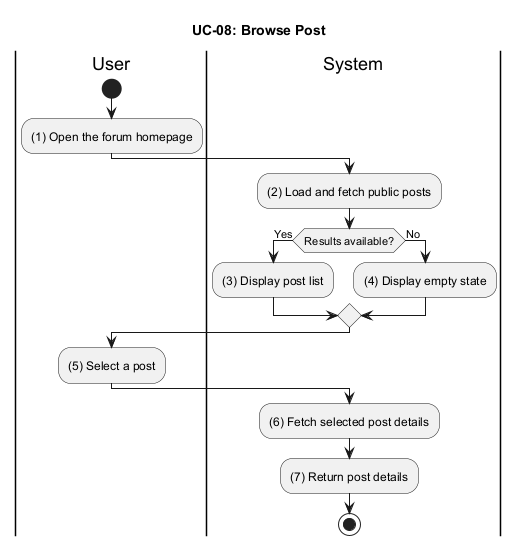
\includegraphics[width=0.8\textwidth]{./diagrams/activity_diagrams/UC_08_Browse_Post.png}
    \caption{Activity Diagram for UC-08}
    \label{fig:ad_uc08}
\end{figure}

\begin{longtblr}[
    caption = {Business Rules for UC-08 - Browse Post},
    label = {tab:uc08_business_rules}
]{
    width=\textwidth,
    hlines,
    vlines,
    rowhead = 1,
    rows = {valign=m, cmd=\nopagebreak},
    row{1} = {font=\bfseries, halign=c},
    colspec = {Q[c,1.8cm] Q[c,1.5cm] Q[c,3.0cm] Q[l,7.5cm]}
}
\textbf{ID} & \textbf{Activity} & \textbf{Rule Type} & \textbf{Description} \\

BR-UC08-01 & (2) & Workflow Rules &
\textbf{Fetch Posts from Database:}
\begin{itemize}
    \item The system calls \textbf{\textit{GetPosts()}} to fetch public posts from the database.
    \item The system fetches authors and communities to enrich the post response.
    \item if \textbf{totalPosts == 0}, then return an empty state instead of an error.
\end{itemize} \\

BR-UC08-02 & (3--4) & Message Rules &
\textbf{Return Content List or Empty State:}
\begin{itemize}
    \item This use case has no dedicated success toast; successful browsing returns content lists or empty states directly in the UI.
    \item Content-loading failures shall use \msgref{community-load-failed}, \msgref{load-posts-failed}, or \msgref{load-avatar-failed}.
    \item Lookup failures shall return \errref{post-not-found}, \errref{community-not-found}, \errref{invalid-id}, or \errref{pagination-invalid}.
\end{itemize} \\

BR-UC08-03 & (6) & Workflow Rules &
\textbf{View Selected Post:}
\begin{itemize}
    \item if the user selects a post, then the system loads the post details using \textbf{\textit{GetPostByID()}}.
    \item if \textbf{userID != null}, then the system also loads \textbf{userVote} and \textbf{userPollVoteIDs}.
\end{itemize} \\

BR-UC08-04 & (6) & Validation Rules &
\textbf{Validate Selected Post Visibility:}
\begin{itemize}
    \item if the selected post is hidden and \textbf{post.AuthorID != userID}, then return post-not-found.
    \item if the selected post is hidden and \textbf{post.AuthorID == userID}, then allow the request to continue.
\end{itemize} \\

BR-UC08-06 & (7) & Message Rules &
\textbf{Return Selected Post:}
\begin{itemize}
    \item The selected post is returned inline when found; this use case does not define a dedicated success toast.
    \item Post-loading failures shall use \msgref{load-posts-failed} and return \errref{post-not-found} or \errref{invalid-id} when applicable.
\end{itemize} \\
\end{longtblr}


\subsection{UC-09 - Search Content}
\begin{table}[H]
\centering
\begin{tblr}{
    width=\textwidth,
    hlines,
    vlines,
    rows = {valign=m},
    colspec = {Q[l,3cm] Q[l,11cm]}
}
\textbf{Name} & Search Content \\
\textbf{Description} & This use case describes how a user searches for posts, users, or communities by keyword. \\
\textbf{Actor} & User \\
\textbf{Trigger} & When the user enters a search term and submits the search. \\
\textbf{Pre-condition} & The search page is available. \newline The system has searchable content. \\
\textbf{Post-condition} & Matching results are returned to the user. \newline The user can open a result or refine the search. \\
\end{tblr}
\caption{Use Case Specification - Search Content}
\end{table}


\begin{figure}[H]
    \centering
    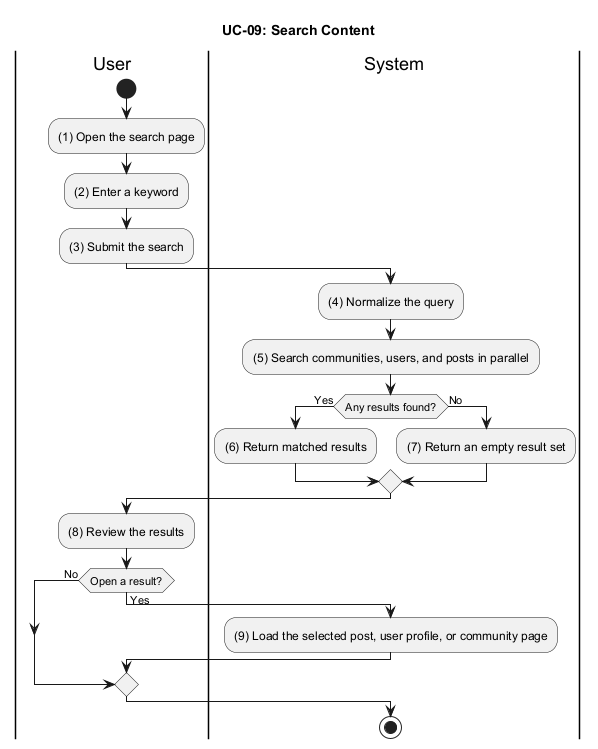
\includegraphics[width=0.65\textwidth]{./diagrams/activity_diagrams/UC_09_Search_Content.png}
    \caption{Activity Diagram for UC-09}
    \label{fig:ad_uc09}
\end{figure}

\begin{longtblr}[
    caption = {Business Rules for UC-09 - Search Content},
    label = {tab:uc09_business_rules}
]{
    width=\textwidth,
    hlines,
    vlines,
    rowhead = 1,
    rows = {valign=m, cmd=\nopagebreak},
    row{1} = {font=\bfseries, halign=c},
    colspec = {Q[c,1.8cm] Q[c,1.5cm] Q[c,3.0cm] Q[l,7.5cm]}
}
\textbf{ID} & \textbf{Activity} & \textbf{Rule Type} & \textbf{Description} \\

BR-UC09-01 & (4) & Validation Rules &
\textbf{Normalize the Query:}
\begin{itemize}
    \item The system decodes the query and removes optional prefixes such as \texttt{c/}, \texttt{lk/}, and \texttt{u/}.
    \item if \textbf{cleanQuery == null} or \textbf{cleanQuery.trim() == ""}, then the system keeps the result sets empty.
\end{itemize} \\

BR-UC09-02 & (5) & Workflow Rules &
\textbf{Search Communities, Users, and Posts in Parallel:}
\begin{itemize}
    \item The system calls \textbf{\textit{GetCommunitiesFilter()}}, \textbf{\textit{GetUsers()}}, and \textbf{\textit{GetPosts()}} through the frontend service layer.
    \item The three requests run in parallel with the same cleaned query.
    \item if any request fails, then the search page clears the result lists and leaves the page in the empty-state path.
\end{itemize} \\

BR-UC09-03 & (6--7) & Message Rules &
\textbf{Return Matched Results or Empty State:}
\begin{itemize}
    \item This use case has no dedicated success toast; matched results or the empty state are rendered directly in the UI.
    \item Search-request failures shall return \errref{bad-request}, \errref{pagination-invalid}, or \errref{invalid-id}.
\end{itemize} \\

BR-UC09-04 & (9) & Redirect Rules &
\textbf{Open Selected Result:}
\begin{itemize}
    \item if the user selects a post, then the system opens the generated post URL.
    \item if the user selects a community, then the system navigates to the community page using \texttt{/lk/\{communityName\}}.
    \item if the user selects a user, then the system navigates to the profile page using \texttt{/profile/\{username\}}.
\end{itemize} \\
\end{longtblr}


\subsection{UC-10 - Create Post}
\begin{table}[H]
\centering
\begin{tblr}{
    width=\textwidth,
    hlines,
    vlines,
    rows = {valign=m},
    colspec = {Q[l,3cm] Q[l,11cm]}
}
\textbf{Name} & Create Post \\
\textbf{Description} & This use case describes how a member creates and submits a new post in a community. \\
\textbf{Actor} & User \\
\textbf{Trigger} & When the user clicks the ``Create Post'' action. \\
\textbf{Pre-condition} & The user is logged in to the system. \newline The user is a member of the selected community. \\
\textbf{Post-condition} & The post is stored successfully. \newline The post appears in the community or enters moderation if required. \\
\end{tblr}
\caption{Use Case Specification - Create Post}
\end{table}


\begin{figure}[H]
    \centering
    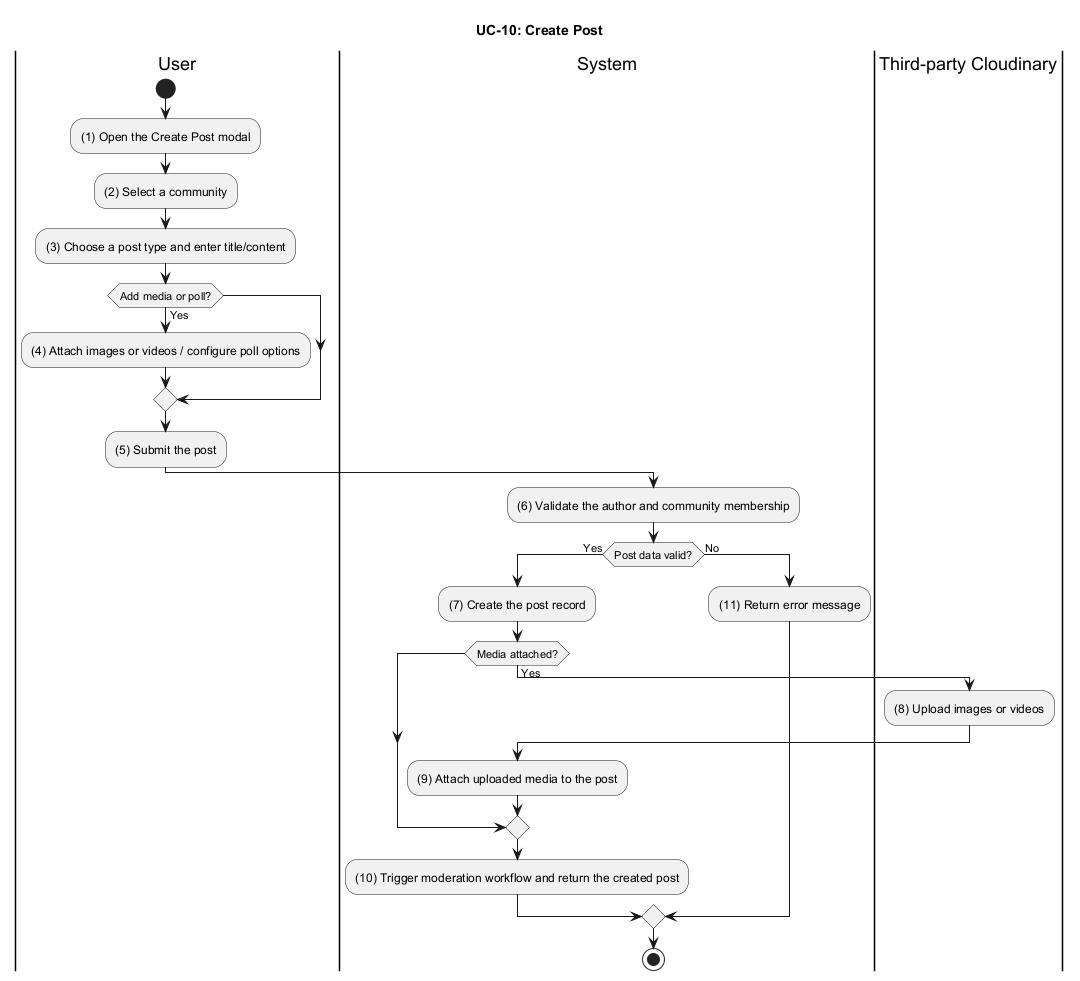
\includegraphics[width=0.8\textwidth]{./diagrams/activity_diagrams/UC_10_Create_Post.png}
    \caption{Activity Diagram for UC-10}
    \label{fig:ad_uc10}
\end{figure}


\begin{longtblr}[
    caption = {Business Rules for UC-10 - Create Post},
    label = {tab:uc10_business_rules}
]{
    width=\textwidth,
    hlines,
    vlines,
    rowhead = 1,
    rows = {valign=m, cmd=\nopagebreak},
    row{1} = {font=\bfseries, halign=c},
    colspec = {Q[c,1.8cm] Q[c,1.5cm] Q[c,3.0cm] Q[l,7.5cm]}
}
\textbf{ID} & \textbf{Activity} & \textbf{Rule Type} & \textbf{Description} \\

BR-UC10-01 & (6) & Validation Rules &
\textbf{Validate Create Post Request:}
\begin{itemize}
    \item if \textbf{authUser == null}, then the controller returns a forbidden response.
    \item if JSON binding fails for \texttt{CreatePostRequest}, then the controller returns a bad request response.
    \item the DTO requires \textbf{community\_id}, \textbf{title}, and \textbf{type}; if any required field is missing, binding fails.
    \item \textbf{type} must be one of \texttt{text}, \texttt{poll}, \texttt{image}, or \texttt{video}.
\end{itemize} \\

BR-UC10-02 & (6) & Authorization Rules &
\textbf{Validate Author and Community Membership:}
\begin{itemize}
    \item if \textbf{communityID == null} or cannot be parsed to an ObjectID, then the service returns an invalid ID error.
    \item if the community does not exist, then the service returns the repository error.
    \item if the author does not exist, then the service returns the repository error.
    \item if \textbf{communityRepo.IsUserBanned() == true}, then the service returns a banned-from-community error.
\end{itemize} \\

BR-UC10-03 & (6) & Workflow Rules &
\textbf{Determine Moderation State:}
\begin{itemize}
    \item if \textbf{author.Role == AdminRole}, then set \textbf{initialStatus = ModerationSkipped}.
    \item if \textbf{community.CreateByID == userID}, then set \textbf{initialStatus = ModerationSkipped}.
    \item if any community moderator has \textbf{mod.UserID == userID}, then set \textbf{initialStatus = ModerationSkipped}.
    \item if \textbf{community.Setting.PostRequireApproval == true} and the author is not admin/mod/creator, then set \textbf{initialStatus = ModerationPending}.
    \item otherwise, set \textbf{initialStatus = ModerationPending} for AI moderation.
\end{itemize} \\

BR-UC10-04 & (7) & Workflow Rules &
\textbf{Create Post Record:}
\begin{itemize}
    \item The system creates a \textbf{Post} with \textbf{AuthorID}, \textbf{CommunityID}, \textbf{Title}, \textbf{Type}, \textbf{Content.text}, \textbf{Tags}, and \textbf{ModerationStatus}.
    \item The system initializes \textbf{VotesCount}, \textbf{CommentsCount}, \textbf{HotScore}, and flag fields such as \textbf{IsDeleted}, \textbf{IsHidden}, \textbf{IsDraft}, and \textbf{IsBan}.
    \item if \textbf{type == poll} and \textbf{req.Poll != null}, then the system creates poll options and attaches poll data to the post content.
    \item The system persists the post through the post repository.
\end{itemize} \\

BR-UC10-05 & (8--9) & Workflow Rules &
\textbf{Attach Media to Post:}
\begin{itemize}
    \item if images are attached, then the system uploads them using \textbf{\textit{UploadImages()}} and pushes them into \textbf{content.images}.
    \item if videos are attached, then the system uploads them using \textbf{\textit{UploadVideos()}} and pushes them into \textbf{content.videos}.
    \item if media upload fails, then the system returns the upload error and does not complete the attach step.
\end{itemize} \\

BR-UC10-06 & (10) & Workflow Rules &
\textbf{Trigger Moderation and Return Post:}
\begin{itemize}
    \item The system increments the author's post count after the post is created.
    \item The system auto-upvotes the post for the creator using \textbf{\textit{VoteOnTargetByAuthor()}}.
    \item The system publishes a post-created event to trigger moderation workflow.
    \item The system returns the created post using \textbf{\textit{GetPostByID()}}.
\end{itemize} \\

BR-UC10-07 & (11) & Message Rules &
\textbf{Return Error Message:}
\begin{itemize}
    \item This use case has no dedicated success toast in the current code; successful post creation returns the created post payload inline.
    \item Validation, membership, or authorization failures shall return \errref{bad-request}, \errref{community-not-found}, \errref{user-not-member}, \errref{banned-community}, \errref{invalid-id}, or \errref{not-authenticated}.
\end{itemize} \\
\end{longtblr}


\subsection{UC-11 - Edit Post}
\begin{table}[H]
\centering
\begin{tblr}{
    width=\textwidth,
    hlines,
    vlines,
    rows = {valign=m},
    colspec = {Q[l,3cm] Q[l,11cm]}
}
\textbf{Name} & Edit Post \\
\textbf{Description} & This use case describes how a member modifies an existing post and preserves edit history. \\
\textbf{Actor} & User \\
\textbf{Trigger} & When the user opens an existing post and chooses ``Edit''. \\
\textbf{Pre-condition} & The user is logged in to the system. \newline The user owns the post or has edit permission. \\
\textbf{Post-condition} & The edited post is saved successfully. \newline The edit history is retained. \\
\end{tblr}
\caption{Use Case Specification - Edit Post}
\end{table}


\begin{figure}[H]
    \centering
    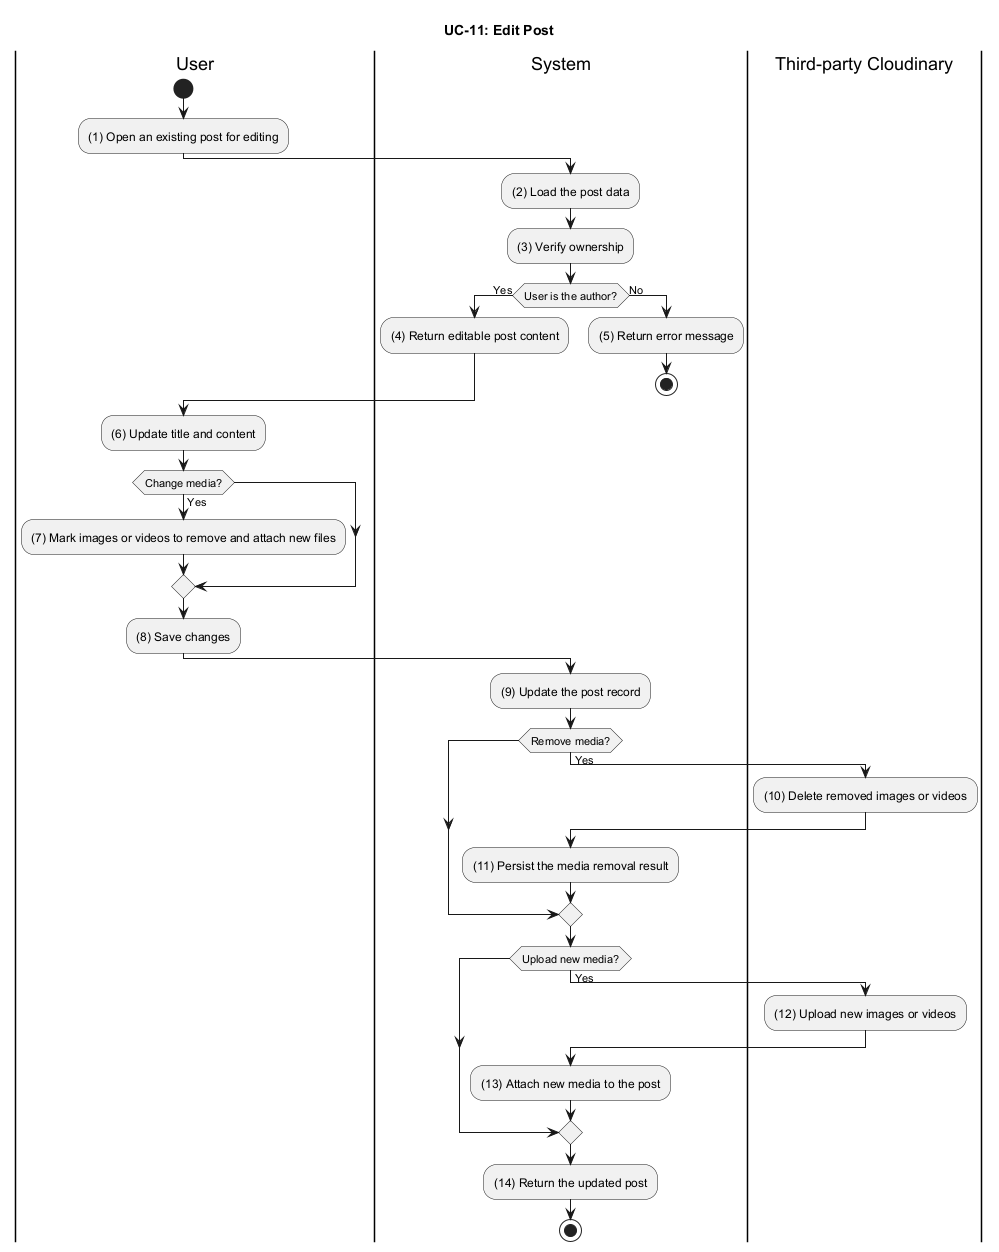
\includegraphics[width=0.65\textwidth]{./diagrams/activity_diagrams/UC_11_Edit_Post.png}
    \caption{Activity Diagram for UC-11}
    \label{fig:ad_uc11}
\end{figure}


\begin{longtblr}[
    caption = {Business Rules for UC-11 - Edit Post},
    label = {tab:uc11_business_rules}
]{
    width=\textwidth,
    hlines,
    vlines,
    rowhead = 1,
    rows = {valign=m, cmd=\nopagebreak},
    row{1} = {font=\bfseries, halign=c},
    colspec = {Q[c,1.8cm] Q[c,1.5cm] Q[c,3.0cm] Q[l,7.5cm]}
}
\textbf{ID} & \textbf{Activity} & \textbf{Rule Type} & \textbf{Description} \\

BR-UC11-01 & (4) & Authorization Rules &
\textbf{Load Post and Verify Ownership:}
\begin{itemize}
    \item The controller requires an authenticated user for the edit request.
    \item if \textbf{authUser == null}, then the controller returns a forbidden response.
    \item if JSON binding fails for \texttt{UpdatePostRequest}, then the controller returns a bad-request response.
    \item The service loads the post by ID and if \textbf{post.AuthorID != userID}, then the service returns a forbidden error.
\end{itemize} \\

BR-UC11-02 & (9) & Workflow Rules &
\textbf{Handle Media Changes Through Post Media Endpoints:}
\begin{itemize}
    \item if the user removes images, then the system calls \textbf{\textit{RemoveImagesFromPost()}} after validating \texttt{public\_ids} and author ownership.
    \item if the user adds images, then the system calls \textbf{\textit{AddImagesToPost()}} and uploads the files with \textbf{\textit{UploadImages()}} before pushing them into \texttt{content.images}.
    \item if the user removes videos, then the system calls \textbf{\textit{RemoveVideosFromPost()}} and deletes the matched Cloudinary assets after the database update.
    \item if the user adds videos, then the system calls \textbf{\textit{AddVideosToPost()}} and uploads the files with \textbf{\textit{UploadVideos()}} before pushing them into \texttt{content.videos}.
    \item if new videos are added, then the system also sets \textbf{type = video}.
\end{itemize} \\

BR-UC11-04 & (10--13) & Workflow Rules &
\textbf{Persist Edit Result and Media Side Effects:}
\begin{itemize}
    \item The system updates the post record with the new content and \textbf{updated\_at} timestamp.
    \item The system publishes a \textbf{PostUpdatedEvent} for moderation.
    \item if image or video upload fails, then the system returns the error and does not finish the edit flow.
    \item if video removal is requested, then the system only removes IDs that already exist in the post.
\end{itemize} \\

BR-UC11-05 & (14) & Message Rules &
\textbf{Return the Updated Post:}
\begin{itemize}
    \item Successful post updates shall use \msgref{update-post-success}; cancellation of unsaved edits shall use \msgref{confirm-discard-changes}.
    \item Failed updates shall use \msgref{update-post-failed}.
    \item Authorization or content-state failures shall return \errref{post-not-found}, \errref{forbidden}, \errref{poll-cannot-edit}, or \errref{invalid-id}.
\end{itemize} \\
\end{longtblr}


\subsection{UC-12 - Delete Post}
\begin{table}[H]
\centering
\begin{tblr}{
    width=\textwidth,
    hlines,
    vlines,
    rows = {valign=m},
    colspec = {Q[l,3cm] Q[l,11cm]}
}
\textbf{Name} & Delete Post \\
\textbf{Description} & This use case describes how a member or moderator removes a post from public view using soft delete. \\
\textbf{Actor} & User / Moderator \\
\textbf{Trigger} & When the user clicks the ``Delete'' action on a post. \\
\textbf{Pre-condition} & The user is logged in to the system. \newline The user has permission to delete the post. \\
\textbf{Post-condition} & The post is marked as deleted. \newline The post is hidden from public view. \\
\end{tblr}
\caption{Use Case Specification - Delete Post}
\end{table}


\begin{figure}[H]
    \centering
    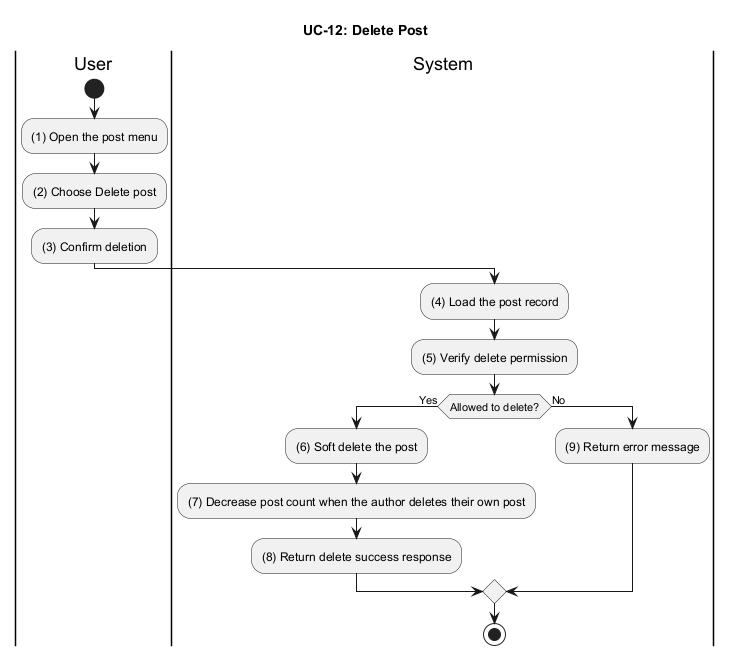
\includegraphics[width=0.7\textwidth]{./diagrams/activity_diagrams/UC_12_Delete_Post.png}
    \caption{Activity Diagram for UC-12}
    \label{fig:ad_uc12}
\end{figure}


\begin{longtblr}[
    caption = {Business Rules for UC-12 - Soft Delete Post},
    label = {tab:uc12_business_rules}
]{
    width=\textwidth,
    hlines,
    vlines,
    rowhead = 1,
    rows = {valign=m, cmd=\nopagebreak},
    row{1} = {font=\bfseries, halign=c},
    colspec = {Q[c,1.8cm] Q[c,1.5cm] Q[c,3.0cm] Q[l,7.5cm]}
}
\textbf{ID} & \textbf{Activity} & \textbf{Rule Type} & \textbf{Description} \\

BR-UC12-01 & (4) & Authorization Rules &
\textbf{Verify Delete Permission:}
\begin{itemize}
    \item The system requires an authenticated user for the delete request.
    \item if \textbf{authUser == null}, then the controller returns an unauthorized response.
    \item The service loads the post by ID and if the post no longer exists, then it returns a post-not-found error.
    \item if \textbf{post.AuthorID == userID}, then the requester may delete their own post.
    \item if \textbf{post.AuthorID != userID}, then the service checks whether the user is an admin, the community creator, or a community moderator.
    \item if none of those permissions exist, then the service returns a forbidden error.
\end{itemize} \\

BR-UC12-02 & (6--7) & Workflow Rules &
\textbf{Soft Delete the Post Record and Adjust Counters:}
\begin{itemize}
    \item The system marks the post as deleted in storage through \textbf{\textit{SoftDelete()}}.
    \item if the author deletes their own post, then the system decreases the author's post count by one.
    \item if the requester is not the author, then the system does not change the author's post count.
\end{itemize} \\

BR-UC12-03 & (8) & Message Rules &
\textbf{Return Success or Error Response:}
\begin{itemize}
    \item Delete confirmation shall use \msgref{confirm-delete-post}; successful deletion shall use \msgref{delete-post-success}.
    \item Failed deletion shall use \msgref{delete-post-failed}.
    \item Permission or lookup failures shall return \errref{post-not-found}, \errref{forbidden}, or \errref{invalid-id}.
\end{itemize} \\

BR-UC12-04 & (9) & Message Rules &
\textbf{Return Success or Error Response:}
\begin{itemize}
    \item The same delete outcome shall reuse \msgref{delete-post-success} on success and \msgref{delete-post-failed} on failure.
    \item Authorization or persistence failures shall return \errref{post-not-found}, \errref{forbidden}, or \errref{invalid-id}.
\end{itemize} \\
\end{longtblr}



\subsection{UC-13 - Post Comment}
\begin{table}[H]
\centering
\begin{tblr}{
    width=\textwidth,
    hlines,
    vlines,
    rows = {valign=m},
    colspec = {Q[l,3cm] Q[l,11cm]}
}
\textbf{Name} & Post Comment \\
\textbf{Description} & This use case describes how a user adds a direct comment to a post. \\
\textbf{Actor} & User \\
\textbf{Trigger} & When the user submits a comment on a post. \\
\textbf{Pre-condition} & The user is logged in to the system. \newline The target post is visible and commentable. \\
\textbf{Post-condition} & The comment is created and attached to the post. \newline The comment count is updated. \\
\end{tblr}
\caption{Use Case Specification - Post Comment}
\end{table}


\begin{figure}[H]
    \centering
    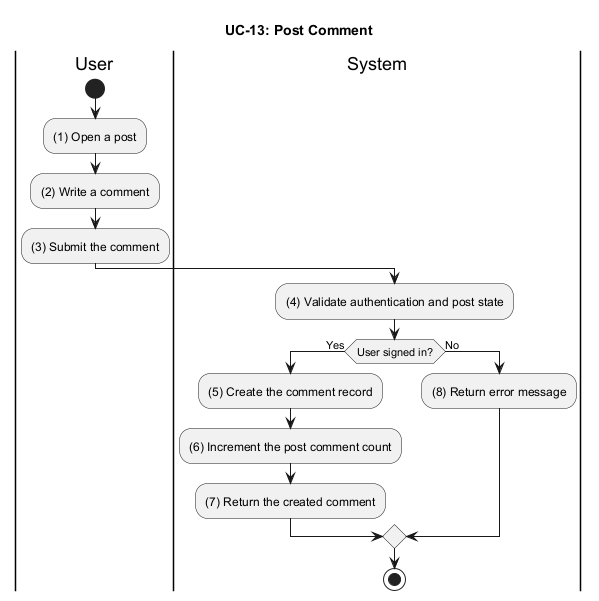
\includegraphics[width=0.8\textwidth]{./diagrams/activity_diagrams/UC_13_Post_Comment.png}
    \caption{Activity Diagram for UC-13}
    \label{fig:ad_uc13}
\end{figure}


\begin{longtblr}[
    caption = {Business Rules for UC-13 - Post Comment},
    label = {tab:uc13_business_rules}
]{
    width=\textwidth,
    hlines,
    vlines,
    rowhead = 1,
    rows = {valign=m, cmd=\nopagebreak},
    row{1} = {font=\bfseries, halign=c},
    colspec = {Q[c,1.8cm] Q[c,1.5cm] Q[c,3.0cm] Q[l,7.5cm]}
}
\textbf{ID} & \textbf{Activity} & \textbf{Rule Type} & \textbf{Description} \\

BR-UC13-01 & (4) & Validation Rules &
\textbf{Validate Request, Post State, and Access:}
\begin{itemize}
    \item The controller binds the request to \texttt{CreateCommentRequest}.
    \item if JSON binding fails, then the controller returns a bad-request response.
    \item \textbf{post\_id} and \textbf{content} are required by the request DTO.
    \item The service loads the target post by \textbf{post\_id}; if the post cannot be found, then the comment flow stops.
    \item The system checks whether the user is muted or banned in the post's community.
    \item if \textbf{authUser == null}, then the controller returns a forbidden response.
    \item if the user is muted or banned, then the service returns the corresponding access error.
\end{itemize} \\

BR-UC13-02 & (4) & Message Rules &
\textbf{Return Bad-Request Message:}
\begin{itemize}
    \item Invalid comment payloads shall return \errref{bad-request}.
\end{itemize} \\

BR-UC13-03 & (5--6) & Workflow Rules &
\textbf{Create Comment and Update Counters:}
\begin{itemize}
    \item The system creates the comment with the current user as author, the selected post as target, and the optional parent comment.
    \item The system stores the new comment with \textbf{IsDeleted = false}.
    \item The system increments the post comment count and the user's comment count.
    \item The system publishes the comment-created event for downstream processing.
\end{itemize} \\

BR-UC13-04 & (7) & Message Rules &
\textbf{Return Created Comment Message:}
\begin{itemize}
    \item Failed comment submission shall use \msgref{comment-post-failed}.
    \item Validation and permission failures shall return \errref{post-not-found}, \errref{user-muted}, \errref{banned-community}, \errref{not-authenticated}, or \errref{invalid-id}.
\end{itemize} \\
\end{longtblr}


\subsection{UC-14 - Reply to Comment}
\begin{table}[H]
\centering
\begin{tblr}{
    width=\textwidth,
    hlines,
    vlines,
    rows = {valign=m},
    colspec = {Q[l,3cm] Q[l,11cm]}
}
\textbf{Name} & Reply to Comment \\
\textbf{Description} & This use case describes how a user replies to an existing comment in a nested discussion thread. \\
\textbf{Actor} & User \\
\textbf{Trigger} & When the user submits a reply to a comment. \\
\textbf{Pre-condition} & The user is logged in to the system. \newline The parent comment exists and can receive replies. \\
\textbf{Post-condition} & The reply is created as a nested comment. \newline The discussion thread is updated. \\
\end{tblr}
\caption{Use Case Specification - Reply to Comment}
\end{table}


\begin{figure}[H]
    \centering
    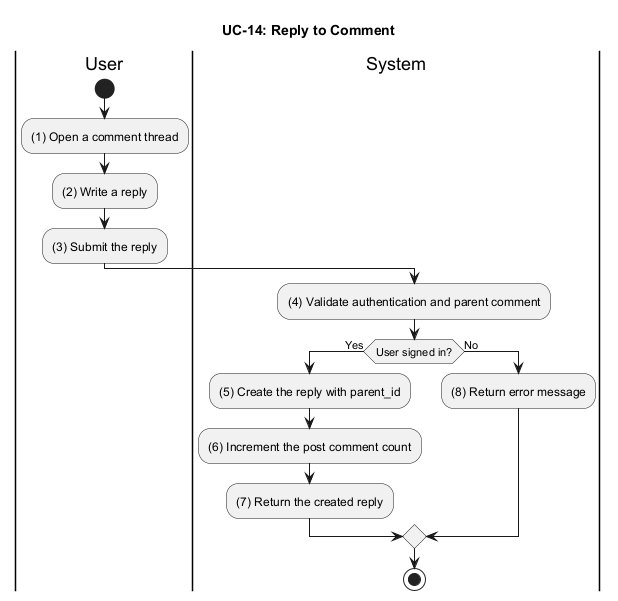
\includegraphics[width=0.6\textwidth]{./diagrams/activity_diagrams/UC_14_Reply_To_Comment.png}
    \caption{Activity Diagram for UC-14}
    \label{fig:ad_uc14}
\end{figure}

\begin{longtblr}[
    caption = {Business Rules for UC-14 - Reply to Comment},
    label = {tab:uc14_business_rules}
]{
    width=\textwidth,
    hlines,
    vlines,
    colspec = {Q[c,1.8cm] Q[c,1.5cm] Q[c,3.0cm] Q[l,7.5cm]}
}
\textbf{ID} & \textbf{Activity} & \textbf{Rule Type} & \textbf{Description} \\

BR-UC14-01 & (4) & Validation Rules &
\textbf{Validate Parent Reply Request and Access:}
\begin{itemize}
    \item The controller binds the request to \texttt{CreateCommentRequest}.
    \item if JSON binding fails, then the controller returns a bad-request response.
    \item \textbf{post\_id} and \textbf{content} are required by the request DTO.
    \item The controller requires an authenticated user before creating the reply.
    \item if \textbf{authUser == null}, then the controller returns a forbidden response.
    \item The service loads the target post by \textbf{post\_id}; if the post cannot be found, then the reply flow stops.
    \item if \textbf{parent\_id} is provided, then the service parses it and uses it as the reply parent when valid.
    \item The system checks whether the user is muted or banned in the post's community.
    \item if the user is muted or banned, then the service returns the corresponding access error.
\end{itemize} \\

BR-UC14-02 & (4) & Message Rules &
\textbf{Return Bad-Request Message:}
\begin{itemize}
    \item Invalid reply payloads shall return \errref{bad-request}.
\end{itemize} \\

BR-UC14-03 & (5--6) & Workflow Rules &
\textbf{Create Reply and Update Counters:}
\begin{itemize}
    \item The system creates the reply with the current user as author, the selected post as target, and the optional parent comment.
    \item The system stores the new reply with \textbf{IsDeleted = false}.
    \item The system increments the post comment count and the user's comment count.
    \item The system publishes the comment-created event for downstream processing.
\end{itemize} \\

BR-UC14-04 & (7) & Message Rules &
\textbf{Return Created Reply Message:}
\begin{itemize}
    \item Failed reply submission shall use \msgref{reply-post-failed}.
    \item Validation and permission failures shall return \errref{comment-not-found}, \errref{post-not-found}, \errref{user-muted}, \errref{depth-too-high}, or \errref{not-authenticated}.
\end{itemize} \\
\end{longtblr}


\subsection{UC-15 - Vote on Content}
\begin{table}[H]
\centering
\begin{tblr}{
    width=\textwidth,
    hlines,
    vlines,
    rows = {valign=m},
    colspec = {Q[l,3cm] Q[l,11cm]}
}
\textbf{Name} & Vote on Content \\
\textbf{Description} & This use case describes how a user upvotes or downvotes a post or comment. \\
\textbf{Actor} & User \\
\textbf{Trigger} & When the user selects an upvote or downvote action. \\
\textbf{Pre-condition} & The user is logged in to the system. \newline The target content is available for voting. \\
\textbf{Post-condition} & The vote is recorded or updated. \newline The content score is recalculated. \\
\end{tblr}
\caption{Use Case Specification - Vote on Content}
\end{table}


\begin{figure}[H]
    \centering
    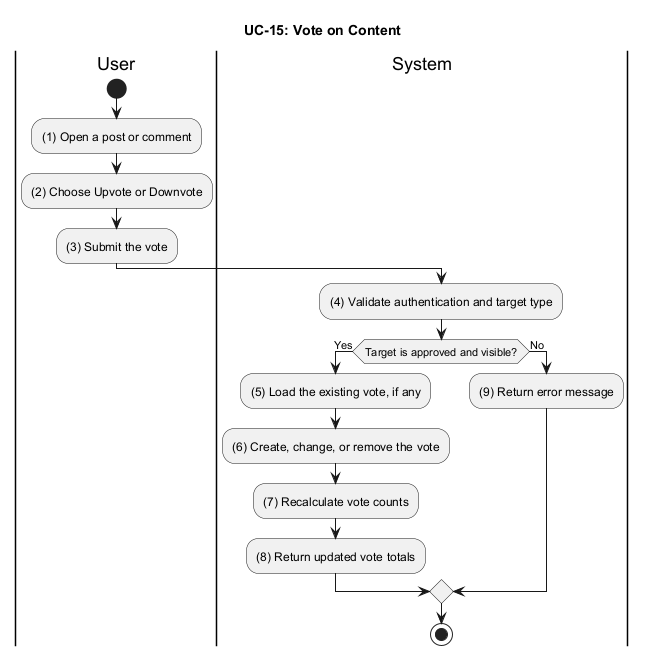
\includegraphics[width=0.8\textwidth]{./diagrams/activity_diagrams/UC_15_Vote_On_Content.png}
    \caption{Activity Diagram for UC-15}
    \label{fig:ad_uc15}
\end{figure}


\begin{longtblr}[
    caption = {Business Rules for UC-15 - Vote on Content},
    label = {tab:uc15_business_rules}
]{
    width=\textwidth,
    hlines,
    vlines,
    rowhead = 1,
    rows = {valign=m, cmd=\nopagebreak},
    row{1} = {font=\bfseries, halign=c},
    colspec = {Q[c,1.8cm] Q[c,1.5cm] Q[c,3.0cm] Q[l,7.5cm]}
}
\textbf{ID} & \textbf{Activity} & \textbf{Rule Type} & \textbf{Description} \\

BR-UC15-01 & (4) & Validation Rules &
\textbf{Validate Authentication, Target Type, and Vote Payload:}
\begin{itemize}
    \item The controller requires an authenticated user before casting or removing a vote.
    \item if \textbf{authUser == null}, then the controller returns an unauthorized response.
    \item The controller accepts only \textbf{post} or \textbf{comment} as \textbf{target\_type}.
    \item if the target type is invalid, then the controller returns a bad-request response.
    \item The controller binds the request body to \texttt{PostVoteRequest}.
    \item if JSON binding fails or \textbf{value == null}, then the controller returns a bad-request response.
\end{itemize} \\

BR-UC15-02 & (4) & Workflow Rules &
\textbf{Check Target Visibility and Load Existing Vote:}
\begin{itemize}
    \item For post voting, the system loads the post and allows voting only when the moderation status is \textbf{approved} or \textbf{skipped}.
    \item For comment voting, the system loads the comment and does not apply a moderation gate.
    \item The system loads the existing vote, if any, before applying the new vote action.
\end{itemize} \\

BR-UC15-03 & (4) & Message Rules &
\textbf{Return Bad-Request Message:}
\begin{itemize}
    \item Invalid vote targets or malformed vote payloads shall return \errref{bad-request}.
\end{itemize} \\

BR-UC15-04 & (5--7) & Workflow Rules &
\textbf{Create, Change, or Remove the Vote:}
\begin{itemize}
    \item if no previous vote exists, then the system creates a new vote record.
    \item if the new value matches the previous value, then the system removes the vote.
    \item if the new value differs from the previous value, then the system updates the existing vote value.
    \item The vote repository updates the target's vote counters inside a transaction.
    \item For post votes, the repository also recalculates \textbf{hot\_score} from the new totals.
\end{itemize} \\

BR-UC15-05 & (8) & Message Rules &
\textbf{Return Updated Vote Totals:}
\begin{itemize}
    \item This use case has no dedicated success toast; the updated upvote, downvote, and score totals are returned inline after the transaction completes.
\end{itemize} \\

BR-UC15-06 & (9) & Message Rules &
\textbf{Return Vote Error Message:}
\begin{itemize}
    \item Poll-vote failures shall use \msgref{poll-vote-failed} or \msgref{poll-unvote-failed}.
    \item Poll-state failures shall return \errref{post-not-found}, \errref{vote-not-found}, \errref{poll-already-voted}, \errref{poll-cannot-edit}, or \errref{not-authenticated}.
\end{itemize} \\
\end{longtblr}



\subsection{UC-16 - Participate in Poll}
\begin{table}[H]
\centering
\begin{tblr}{
    width=\textwidth,
    hlines,
    vlines,
    rows = {valign=m},
    colspec = {Q[l,3cm] Q[l,11cm]}
}
\textbf{Name} & Participate in Poll \\
\textbf{Description} & This use case describes how a user casts a vote in a community poll. \\
\textbf{Actor} & User \\
\textbf{Trigger} & When the user submits a poll vote. \\
\textbf{Pre-condition} & The user is logged in to the system. \newline The poll is open for voting. \\
\textbf{Post-condition} & The selected poll option is recorded. \newline The poll results are updated. \\
\end{tblr}
\caption{Use Case Specification - Participate in Poll}
\end{table}


\begin{figure}[H]
    \centering
    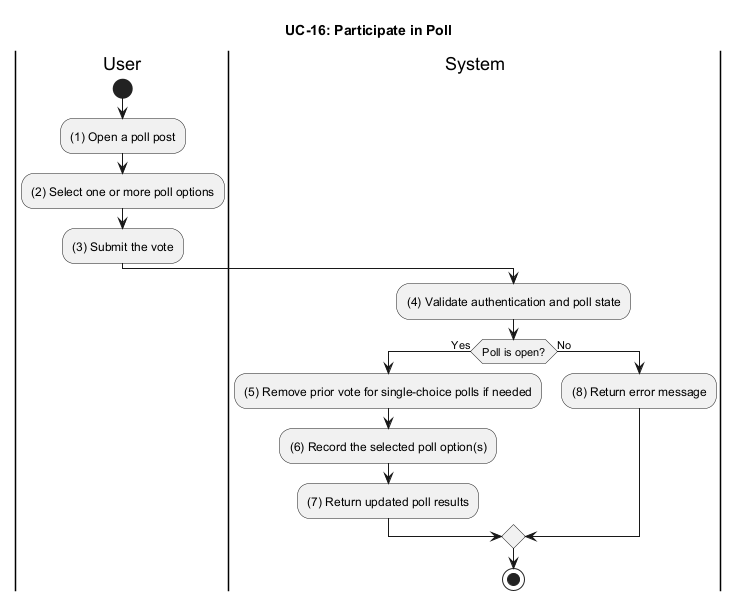
\includegraphics[width=\textwidth]{./diagrams/activity_diagrams/UC_16_Participate_In_Poll.png}
    \caption{Activity Diagram for UC-16}
    \label{fig:ad_uc16}
\end{figure}


\begin{longtblr}[
    caption = {Business Rules for UC-16 - Participate in Poll},
    label = {tab:uc16_business_rules}
]{
    width=\textwidth,
    hlines,
    vlines,
    rowhead = 1,
    rows = {valign=m, cmd=\nopagebreak},
    row{1} = {font=\bfseries, halign=c},
    colspec = {Q[c,1.8cm] Q[c,1.5cm] Q[c,3.0cm] Q[l,7.5cm]}
}
\textbf{ID} & \textbf{Activity} & \textbf{Rule Type} & \textbf{Description} \\

BR-UC16-01 & (4) & Validation Rules &
\textbf{Validate Authentication, Poll State, and Vote Payload:}
\begin{itemize}
    \item The controller requires an authenticated user before recording a poll vote.
    \item if \textbf{authUser == null}, then the controller returns an unauthorized response.
    \item The controller binds the request body to \texttt{PollVoteRequest}.
    \item if JSON binding fails or \textbf{option\_id} is missing, then the controller returns a bad-request response.
    \item The service loads the target post and requires it to contain poll content.
    \item if the post cannot be found, is not a poll, or does not contain poll data, then the service returns an error.
\end{itemize} \\

BR-UC16-02 & (4) & Message Rules &
\textbf{Return Bad-Request Message:}
\begin{itemize}
    \item Invalid poll-vote payloads shall return \errref{bad-request}.
\end{itemize} \\

BR-UC16-03 & (5--6) & Workflow Rules &
\textbf{Record the Poll Vote:}
\begin{itemize}
    \item The repository loads the user's existing poll votes for the post.
    \item if the poll is single-choice and the user already voted another option, then the repository removes the previous vote before adding the new one.
    \item if the selected option was already voted by the user, then the repository removes that specific vote instead of adding a duplicate.
    \item The repository stores the new poll vote and increments the selected option vote count plus the poll total votes.
\end{itemize} \\

BR-UC16-04 & (7) & Workflow Rules &
\textbf{Return Updated Poll Results:}
\begin{itemize}
    \item The service reloads the poll and user vote IDs after the transaction completes.
    \item The system returns the refreshed poll response with updated totals and user vote IDs.
\end{itemize} \\

BR-UC16-05 & (7) & Message Rules &
\textbf{Return Created Poll Vote Message:}
\begin{itemize}
    \item This use case has no dedicated success toast in the current code; the updated poll payload is returned inline after a successful vote.
\end{itemize} \\

BR-UC16-06 & (8) & Message Rules &
\textbf{Return Poll Vote Error Message:}
\begin{itemize}
    \item Poll-vote failures shall use \msgref{poll-vote-failed} or \msgref{poll-unvote-failed}.
    \item Poll-state failures shall return \errref{post-not-found}, \errref{vote-not-found}, \errref{poll-already-voted}, \errref{poll-cannot-edit}, or \errref{not-authenticated}.
\end{itemize} \\
\end{longtblr}


\subsection{UC-17 - Save Post}
\begin{table}[H]
\centering
\begin{tblr}{
    width=\textwidth,
    hlines,
    vlines,
    rows = {valign=m},
    colspec = {Q[l,3cm] Q[l,11cm]}
}
\textbf{Name} & Save Post \\
\textbf{Description} & This use case describes how a user bookmarks a post for later viewing. \\
\textbf{Actor} & User \\
\textbf{Trigger} & When the user clicks the ``Save'' action on a post. \\
\textbf{Pre-condition} & The user is logged in to the system. \newline The target post exists and is visible to the user. \\
\textbf{Post-condition} & The post is added to the user's saved list. \newline The saved state is available in the account. \\
\end{tblr}
\caption{Use Case Specification - Save Post}
\end{table}


\begin{figure}[H]
    \centering
    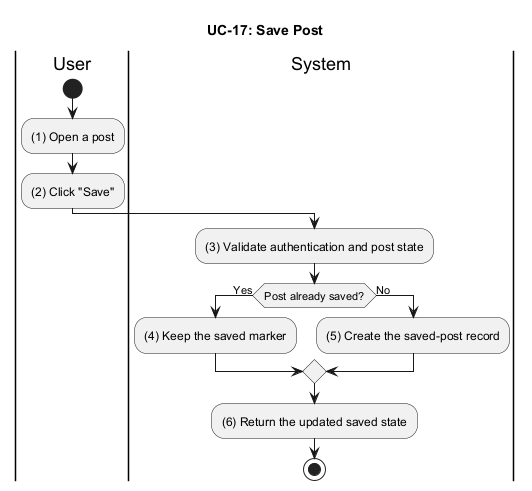
\includegraphics[width=0.8\textwidth]{./diagrams/activity_diagrams/UC_17_Save_Post.png}
    \caption{Activity Diagram for UC-17}
    \label{fig:ad_uc17}
\end{figure}


\begin{longtblr}[
    caption = {Business Rules for UC-17 - Save Post},
    label = {tab:uc17_business_rules}
]{
    width=\textwidth,
    hlines,
    vlines,
    rowhead = 1,
    rows = {valign=m, cmd=\nopagebreak},
    row{1} = {font=\bfseries, halign=c},
    colspec = {Q[c,1.8cm] Q[c,1.5cm] Q[c,3.0cm] Q[l,7.5cm]}
}
\textbf{ID} & \textbf{Activity} & \textbf{Rule Type} & \textbf{Description} \\

BR-UC17-01 & (3) & Validation Rules &
\textbf{Validate Authentication and Post ID:}
\begin{itemize}
    \item The controller requires an authenticated user before saving a post.
    \item if \textbf{authUser == null}, then the controller returns a forbidden response.
    \item The service parses the user ID and post ID to ObjectIDs.
    \item if either ID cannot be parsed, then the service returns an invalid-ID error.
\end{itemize} \\

BR-UC17-02 & (3) & Workflow Rules &
\textbf{Check Post State and Save Relation:}
\begin{itemize}
    \item The service loads the post before saving it.
    \item if the post cannot be found, then the service returns the post lookup error.
    \item The saved-post repository stores the relation with upsert semantics so an existing saved marker is kept instead of duplicated.
\end{itemize} \\

BR-UC17-03 & (4--5) & Workflow Rules &
\textbf{Create or Keep the Saved Marker:}
\begin{itemize}
    \item if the post is already saved by the user, then the system keeps the saved marker unchanged.
    \item if the post is not yet saved, then the system creates the saved-post record.
\end{itemize} \\

BR-UC17-04 & (6) & Message Rules &
\textbf{Return Updated Saved State:}
\begin{itemize}
    \item This use case has no dedicated success toast in the current code; the updated saved state is returned inline after the relation is stored.
\end{itemize} \\

BR-UC17-05 & (6) & Message Rules &
\textbf{Return Save Error Message:}
\begin{itemize}
    \item Save-post failures shall return \errref{not-authenticated}, \errref{invalid-id}, \errref{post-not-found}, or \errref{forbidden}.
\end{itemize} \\
\end{longtblr}



\subsection{UC-18 - Hide Post}
\begin{table}[H]
\centering
\begin{tblr}{
    width=\textwidth,
    hlines,
    vlines,
    rows = {valign=m},
    colspec = {Q[l,3cm] Q[l,11cm]}
}
\textbf{Name} & Hide Post \\
\textbf{Description} & This use case describes how a user hides a post from their personal feed. \\
\textbf{Actor} & User \\
\textbf{Trigger} & When the user clicks the ``Hide'' action on a post. \\
\textbf{Pre-condition} & The user is logged in to the system. \newline The target post is visible in the user's feed. \\
\textbf{Post-condition} & The post is hidden from the user's feed. \newline The hidden-post record is stored for the account. \\
\end{tblr}
\caption{Use Case Specification - Hide Post}
\end{table}


\begin{figure}[H]
    \centering
    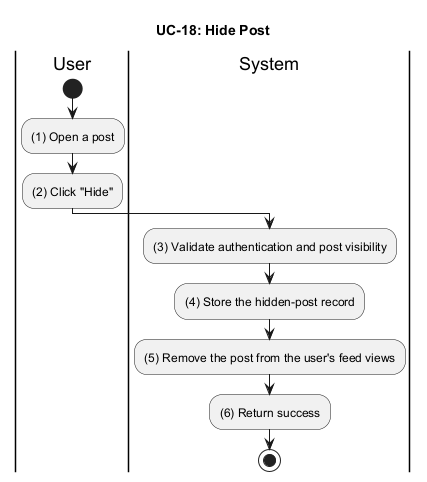
\includegraphics[width=0.8\textwidth]{./diagrams/activity_diagrams/UC_18_Hide_Post.png}
    \caption{Activity Diagram for UC-18}
    \label{fig:ad_uc18}
\end{figure}


\begin{longtblr}[
    caption = {Business Rules for UC-18 - Hide Post},
    label = {tab:uc18_business_rules}
]{
    width=\textwidth,
    hlines,
    vlines,
    rowhead = 1,
    rows = {valign=m, cmd=\nopagebreak},
    row{1} = {font=\bfseries, halign=c},
    colspec = {Q[c,1.8cm] Q[c,1.5cm] Q[c,3.0cm] Q[l,7.5cm]}
}
\textbf{ID} & \textbf{Activity} & \textbf{Rule Type} & \textbf{Description} \\

BR-UC18-01 & (3) & Validation Rules &
\textbf{Validate Authentication and Post Ownership:}
\begin{itemize}
    \item The controller requires an authenticated user before hiding a post.
    \item if \textbf{authUser == null}, then the controller returns a forbidden response.
    \item The service loads the post by ID before hiding it.
    \item if the post cannot be found, then the service returns the post lookup error.
    \item if the authenticated user is not the post author, then the service returns a forbidden error.
\end{itemize} \\

BR-UC18-02 & (4--5) & Workflow Rules &
\textbf{Mark the Post Hidden and Remove It From Visible Feeds:}
\begin{itemize}
    \item The service updates the post record by setting \textbf{is\_hidden = true}.
    \item The hidden marker keeps the post out of normal feed queries because feed filters exclude hidden posts.
\end{itemize} \\

BR-UC18-03 & (6) & Message Rules &
\textbf{Return Hide Success Message:}
\begin{itemize}
    \item This use case has no dedicated success toast in the current code; the updated hidden state is returned inline after storage.
\end{itemize} \\

BR-UC18-04 & (6) & Message Rules &
\textbf{Return Hide Error Message:}
\begin{itemize}
    \item Hide-post failures shall return \errref{not-authenticated}, \errref{forbidden}, \errref{invalid-id}, or \errref{post-not-found}.
\end{itemize} \\
\end{longtblr}



\subsection{UC-19 - Manage Drafts}
\begin{table}[H]
\centering
\begin{tblr}{
    width=\textwidth,
    hlines,
    vlines,
    rows = {valign=m},
    colspec = {Q[l,3cm] Q[l,11cm]}
}
\textbf{Name} & Manage Drafts \\
\textbf{Description} & This use case describes how a user saves unfinished posts as drafts and publishes them later. \\
\textbf{Actor} & User \\
\textbf{Trigger} & When the user saves, edits, opens, or publishes a draft. \\
\textbf{Pre-condition} & The user is logged in to the system. \newline The user has draft access. \\
\textbf{Post-condition} & The draft is saved, updated, or deleted after publishing. \newline A published draft becomes a normal post. \\
\end{tblr}
\caption{Use Case Specification - Manage Drafts}
\end{table}


\begin{figure}[H]
    \centering
    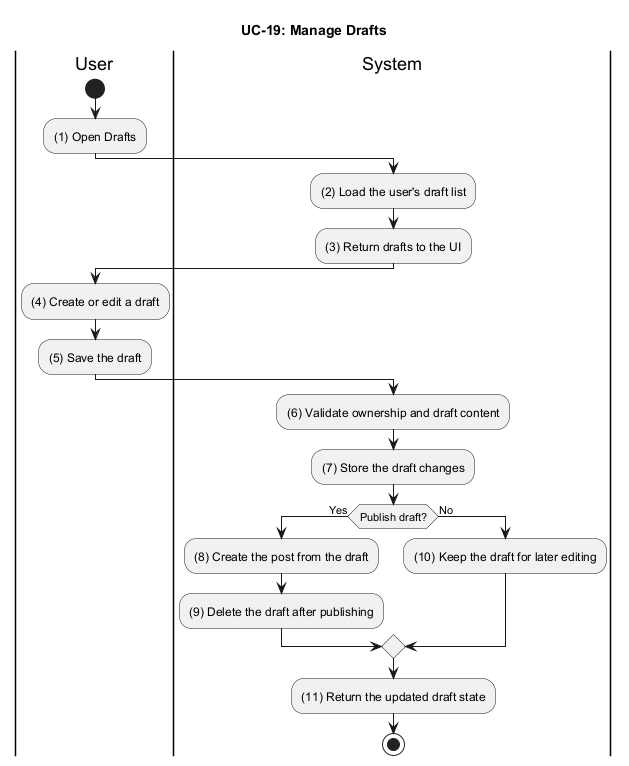
\includegraphics[width=0.7\textwidth]{./diagrams/activity_diagrams/UC_19_Manage_Drafts.png}
    \caption{Activity Diagram for UC-19}
    \label{fig:ad_uc19}
\end{figure}


\begin{longtblr}[
    caption = {Business Rules for UC-19 - Manage Drafts},
    label = {tab:uc19_business_rules}
]{
    width=\textwidth,
    hlines,
    vlines,
    rowhead = 1,
    rows = {valign=m, cmd=\nopagebreak},
    row{1} = {font=\bfseries, halign=c},
    colspec = {Q[c,1.8cm] Q[c,1.5cm] Q[c,3.0cm] Q[l,7.5cm]}
}
\textbf{ID} & \textbf{Activity} & \textbf{Rule Type} & \textbf{Description} \\

BR-UC19-01 & (2--3) & Workflow Rules &
\textbf{Load the User's Draft List:}
\begin{itemize}
    \item The service loads drafts by author using \textbf{\textit{GetDraftsByAuthor()}}.
    \item The service returns the draft summaries with pagination metadata.
\end{itemize} \\

BR-UC19-02 & (6) & Authorization Rules &
\textbf{Validate Draft Ownership and Payload:}
\begin{itemize}
    \item The controller requires an authenticated user before draft operations.
    \item if \textbf{authUser == null}, then the controller returns a forbidden response.
    \item The service parses the author ID and draft ID to ObjectIDs.
    \item if either ID cannot be parsed, then the service returns an invalid-ID error.
    \item The service loads the draft and if the draft author does not match the requester, then the service returns a forbidden error.
\end{itemize} \\

BR-UC19-03 & (6--7) & Workflow Rules &
\textbf{Store Draft Changes:}
\begin{itemize}
    \item The service creates or updates the draft record with community, type, title, text, tags, images, videos, and poll data.
    \item The draft record updates \textbf{UpdatedAt} whenever changes are saved.
    \item if the draft does not exist or the author is invalid, then the operation stops before saving.
\end{itemize} \\

BR-UC19-04 & (8--10) & Workflow Rules &
\textbf{Publish or Keep the Draft:}
\begin{itemize}
    \item if publish is requested, then the service validates that title, community, and type are present.
    \item The service creates a post from the draft using \textbf{\textit{CreatePost()}}.
    \item After a successful publish, the service deletes the draft record.
    \item if publish is not requested, then the service keeps the draft for later editing.
\end{itemize} \\

BR-UC19-05 & (11) & Message Rules &
\textbf{Return Updated Draft State:}
\begin{itemize}
    \item Draft actions shall use \msgref{save-draft-success}, \msgref{confirm-delete-draft}, \msgref{delete-draft-failed}, and \msgref{draft-load-failed} where applicable.
    \item Successful publish or update responses may return the updated draft or post inline without a dedicated additional toast.
\end{itemize} \\

BR-UC19-06 & (11) & Message Rules &
\textbf{Return Draft Error Message:}
\begin{itemize}
    \item Draft validation or lookup failures shall return \errref{draft-not-found}, \errref{invalid-id}, \errref{not-authenticated}, \errref{community-not-found}, or \errref{user-not-member}.
\end{itemize} \\
\end{longtblr}


\subsection{UC-20 - Private Messaging}
\begin{table}[H]
\centering
\begin{tblr}{
    width=\textwidth,
    hlines,
    vlines,
    rows = {valign=m},
    colspec = {Q[l,3cm] Q[l,11cm]}
}
\textbf{Name} & Private Messaging \\
\textbf{Description} & This use case describes how users exchange instant one-to-one messages through the messaging system. \\
\textbf{Actor} & User \\
\textbf{Trigger} & When the user opens a conversation and sends a message. \\
\textbf{Pre-condition} & The user is logged in to the system. \newline The conversation channel exists and is accessible. \\
\textbf{Post-condition} & The message is delivered to the conversation members. \newline The channel read state is updated. \\
\end{tblr}
\caption{Use Case Specification - Private Messaging}
\end{table}


\begin{figure}[H]
    \centering
    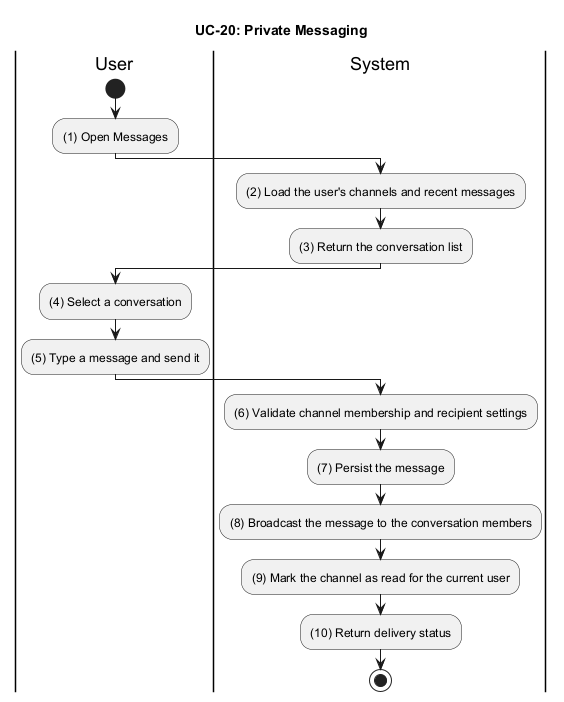
\includegraphics[width=0.8\textwidth]{./diagrams/activity_diagrams/UC_20_Private_Messaging.png}
    \caption{Activity Diagram for UC-20}
    \label{fig:ad_uc20}
\end{figure}


\begin{longtblr}[
    caption = {Business Rules for UC-20 - Private Messaging},
    label = {tab:uc20_business_rules}
]{
    width=\textwidth,
    hlines,
    vlines,
    rowhead = 1,
    rows = {valign=m, cmd=\nopagebreak},
    row{1} = {font=\bfseries, halign=c},
    colspec = {Q[c,1.8cm] Q[c,1.5cm] Q[c,3.0cm] Q[l,7.5cm]}
}
\textbf{ID} & \textbf{Activity} & \textbf{Rule Type} & \textbf{Description} \\

BR-UC20-01 & (2) & Authorization Rules &
\textbf{Load the User's Conversations:}
\begin{itemize}
    \item The controller requires an authenticated user before loading conversation data.
    \item if \textbf{authUser == null}, then the controller returns a forbidden response.
    \item The channel service only returns channels when the requester matches the target user ID.
    \item if the requester is not the same as the target user, then the service returns a forbidden error.
\end{itemize} \\

BR-UC20-02 & (2--3) & Workflow Rules &
\textbf{Return Conversation List and Recent Message State:}
\begin{itemize}
    \item The service loads the user's channels using \textbf{\textit{GetChannelsByUserID()}}.
    \item The service returns the conversation list together with pagination data.
    \item The message filter endpoint returns the user's messages only when the requester is a member of the channel.
\end{itemize} \\

BR-UC20-03 & (6) & Validation Rules &
\textbf{Validate New Message Payload and Channel Access:}
\begin{itemize}
    \item The websocket hub decodes the \texttt{new_message} payload before publishing the event.
    \item if the payload is malformed or required fields are missing, then the hub sends an error message back to the sender.
    \item The message service validates that \textbf{temp\_message\_id}, \textbf{channel\_id}, \textbf{sender\_id}, \textbf{sender\_username}, and \textbf{content} are present.
    \item The service loads the target channel and verifies that the sender is a member of that channel.
    \item The service checks each recipient's direct-message setting before continuing.
\end{itemize} \\

BR-UC20-04 & (7--8) & Workflow Rules &
\textbf{Persist and Broadcast the Message:}
\begin{itemize}
    \item The service creates a \texttt{Message} with \textbf{IsSend = false}, \textbf{IsRead = false}, and \textbf{IsDeleted = false}.
    \item The repository stores the message and returns the created record.
    \item The message service publishes a broadcast event so the websocket hub can send an ACK to the sender and a delivery event to the recipients.
    \item if persistence fails, then the service publishes a message error event instead of broadcasting success.
\end{itemize} \\

BR-UC20-05 & (9) & Workflow Rules &
\textbf{Mark the Channel as Read:}
\begin{itemize}
    \item The message service marks the channel as read only for channel members.
    \item The repository updates unread messages to \textbf{is\_read = true} for messages not sent by the current user.
\end{itemize} \\

BR-UC20-06 & (10) & Message Rules &
\textbf{Return Delivery Status:}
\begin{itemize}
    \item Successful message delivery returns the stored payload inline through the websocket ACK and broadcast flow; this use case does not define a dedicated success toast.
\end{itemize} \\

BR-UC20-07 & (10) & Message Rules &
\textbf{Return Messaging Error:}
\begin{itemize}
    \item Message-delivery failures shall use \msgref{send-message-failed}, \msgref{create-channel-failed}, or \msgref{open-chat-failed}.
    \item Channel and access failures shall return \errref{channel-not-found}, \errref{no-message-found}, \errref{forbidden}, \errref{invalid-id}, or \errref{not-authenticated}.
\end{itemize} \\
\end{longtblr}



\subsection{UC-21 - Manage Notifications}
\begin{table}[H]
\centering
\begin{tblr}{
    width=\textwidth,
    hlines,
    vlines,
    rows = {valign=m},
    colspec = {Q[l,3cm] Q[l,11cm]}
}
\textbf{Name} & Manage Notifications \\
\textbf{Description} & This use case describes how a user views and clears system notifications. \\
\textbf{Actor} & User \\
\textbf{Trigger} & When the user opens the notifications page or marks notifications as read. \\
\textbf{Pre-condition} & The user is logged in to the system. \newline Notifications exist for the account. \\
\textbf{Post-condition} & The selected notifications are marked as read or deleted. \newline The notification list is refreshed. \\
\end{tblr}
\caption{Use Case Specification - Manage Notifications}
\end{table}


\begin{figure}[H]
    \centering
    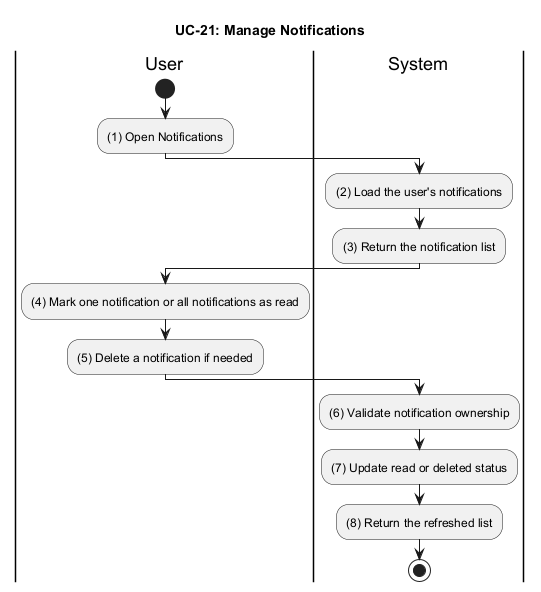
\includegraphics[width=0.7\textwidth]{./diagrams/activity_diagrams/UC_21_Manage_Notifications.png}
    \caption{Activity Diagram for UC-21}
    \label{fig:ad_uc21}
\end{figure}


\begin{longtblr}[
    caption = {Business Rules for UC-21 - Manage Notifications},
    label = {tab:uc21_business_rules}
]{
    width=\textwidth,
    hlines,
    vlines,
    rowhead = 1,
    rows = {valign=m, cmd=\nopagebreak},
    row{1} = {font=\bfseries, halign=c},
    colspec = {Q[c,1.8cm] Q[c,1.5cm] Q[c,3.0cm] Q[l,7.5cm]}
}
\textbf{ID} & \textbf{Activity} & \textbf{Rule Type} & \textbf{Description} \\

\textbf{BR-UC21-01} & (2--3) & Workflow Rules &
\textbf{Load Notifications:}
\begin{itemize}
    \item The system loads notifications for \textbf{recipientID} using \textbf{\textit{GetNotifications()}}.
    \item The system returns the notification list with pagination data.
\end{itemize} \\

\textbf{BR-UC21-02} & (6) & Authorization Rules &
\textbf{Validate Notification Ownership:}
\begin{itemize}
    \item The notification routes require authentication before any operation is processed.
    \item The system only updates or deletes notifications that belong to the authenticated user.
    \item If the notification ID is missing or the current user does not own the record, the operation is rejected.
\end{itemize} \\

\textbf{BR-UC21-03} & (6) & Validation Rules &
\textbf{Validate Notification ID for Single-Item Actions:}
\begin{itemize}
    \item If the user marks one notification as read or deletes one notification, the system validates \textbf{notificationID}.
    \item The service converts \textbf{notificationID} to an object ID before calling the repository.
\end{itemize} \\

\textbf{BR-UC21-04} & (7) & Workflow Rules &
\textbf{Update Notification State:}
\begin{itemize}
    \item If the user marks all notifications as read, the system updates them using \textbf{\textit{MarkAllAsRead()}}.
    \item If the user marks a single notification as read, the system updates it using \textbf{\textit{MarkAsRead()}}.
    \item If the user deletes a notification, the system removes it using \textbf{\textit{DeleteNotification()}}.
    \item The repository filters updates by both notification ID and recipient ID.
\end{itemize} \\

\textbf{BR-UC21-05} & (8) & Message Rules &
\textbf{Return the Refreshed Notification List:}
\begin{itemize}
    \item Notification-related UI feedback shall use \msgref{notifications-load-failed}, \msgref{accept-moderator-success}, or \msgref{accept-invitation-failed} when the notification action is an invitation.
    \item Successful notification-state changes may return the refreshed list inline without a dedicated additional toast.
\end{itemize} \\

\textbf{BR-UC21-06} & (8) & Message Rules &
\textbf{Return Notification Error Message:}
\begin{itemize}
    \item Notification access or lookup failures shall return \errref{invalid-id}, \errref{forbidden}, \errref{not-authenticated}, or \errref{invalid-token}.
\end{itemize} \\
\end{longtblr}



\subsection{UC-22 - Report Violation}
\begin{table}[H]
\centering
\begin{tblr}{
    width=\textwidth,
    hlines,
    vlines,
    rows = {valign=m},
    colspec = {Q[l,3cm] Q[l,11cm]}
}
\textbf{Name} & Report Violation \\
\textbf{Description} & This use case describes how a user reports inappropriate content or behavior for review. \\
\textbf{Actor} & User \\
\textbf{Trigger} & When the user submits a report form. \\
\textbf{Pre-condition} & The user is logged in to the system. \newline The reported target is available. \\
\textbf{Post-condition} & The report is stored in the moderation queue. \newline The report can be reviewed by moderators or admins. \\
\end{tblr}
\caption{Use Case Specification - Report Violation}
\end{table}


\begin{figure}[H]
    \centering
    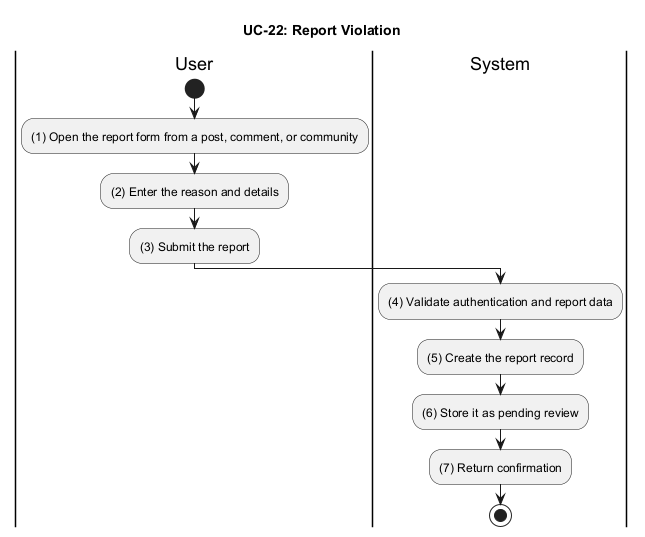
\includegraphics[width=0.8\textwidth]{./diagrams/activity_diagrams/UC_22_Report_Violation.png}
    \caption{Activity Diagram for UC-22}
    \label{fig:ad_uc22}
\end{figure}


\begin{longtblr}[
    caption = {Business Rules for UC-22 - Report Violation},
    label = {tab:uc22_business_rules}
]{
    width=\textwidth,
    hlines,
    vlines,
    rowhead = 1,
    rows = {valign=m, cmd=\nopagebreak},
    row{1} = {font=\bfseries, halign=c},
    colspec = {Q[c,1.8cm] Q[c,1.5cm] Q[c,3.0cm] Q[l,7.5cm]}
}
\textbf{ID} & \textbf{Activity} & \textbf{Rule Type} & \textbf{Description} \\

BR-UC22-01 & (4) & Authorization / Validation Rules &
\textbf{Submit Report Request:}
\begin{itemize}
    \item The report action requires an authenticated user.
    \item The report form is opened from a post detail or post card action.
    \item The controller binds the JSON body to \texttt{ReportPostRequest}.
    \item The submitted \textbf{reason} is required.
    \item The submitted \textbf{description} is optional.
    \item if \textbf{authUser == null}, then return a forbidden response.
    \item if the payload is invalid, then return a bad request response.
\end{itemize} \\

BR-UC22-02 & (4) & Validation Rules &
\textbf{Validate the Target Post:}
\begin{itemize}
    \item The service parses \textbf{reporterID} and \textbf{postID} to object IDs.
    \item The service loads the target post before creating the report.
    \item if the post does not exist or the IDs are invalid, then stop the operation and return the corresponding error.
\end{itemize} \\

BR-UC22-03 & (4) & Constraint Rules &
\textbf{Prevent Invalid Reports:}
\begin{itemize}
    \item The system rejects reports submitted by the author of the target post.
    \item The system rejects duplicate reports from the same user for the same post.
\end{itemize} \\

BR-UC22-04 & (5--6) & Workflow Rules &
\textbf{Create and Store the Report:}
\begin{itemize}
    \item The service creates a \texttt{Report} with \textbf{TargetType = post}.
    \item The repository stores the report with \textbf{IsDeleted = false}.
    \item The report remains pending until reviewed by moderators or administrators.
\end{itemize} \\

BR-UC22-05 & (7) & Message Rules &
\textbf{Return Operation Result:}
\begin{itemize}
    \item Report submission shall use \msgref{report-sent-success} on success and \msgref{report-sent-failed} on failure.
    \item Report validation failures shall return \errref{already-reported}, \errref{post-not-found}, \errref{comment-not-found}, \errref{user-not-found}, \errref{invalid-id}, or \errref{not-authenticated}.
\end{itemize} \\
\end{longtblr}

\subsection{UC-23 - Create Community}
\begin{table}[H]
\centering
\begin{tblr}{
    width=\textwidth,
    hlines,
    vlines,
    rows = {valign=m},
    colspec = {Q[l,3cm] Q[l,11cm]}
}
\textbf{Name} & Create Community \\
\textbf{Description} & This use case describes how a user creates a new community and becomes its owner. \\
\textbf{Actor} & User \\
\textbf{Trigger} & When the user submits the create community form. \\
\textbf{Pre-condition} & The user is logged in to the system. \newline The community name is available and valid. \\
\textbf{Post-condition} & The community is created successfully. \newline The creator becomes the owner and first member. \\
\end{tblr}
\caption{Use Case Specification - Create Community}
\end{table}


\begin{figure}[H]
    \centering
    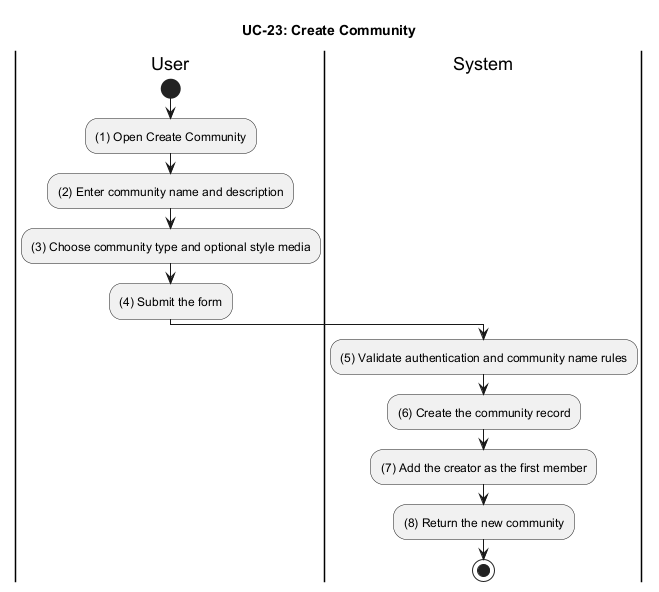
\includegraphics[width=0.8\textwidth]{./diagrams/activity_diagrams/UC_23_Create_Community.png}
    \caption{Activity Diagram for UC-23}
    \label{fig:ad_uc23}
\end{figure}


\begin{longtblr}[
    caption = {Business Rules for UC-23 - Create Community},
    label = {tab:uc23_business_rules}
]{
    width=\textwidth,
    hlines,
    vlines,
    rowhead = 1,
    rows = {valign=m, cmd=\nopagebreak},
    row{1} = {font=\bfseries, halign=c},
    colspec = {Q[c,1.8cm] Q[c,1.5cm] Q[c,3.0cm] Q[l,7.5cm]}
}
\textbf{ID} & \textbf{Activity} & \textbf{Rule Type} & \textbf{Description} \\

BR-UC23-01 & (5) & Authorization Rules &
\textbf{Open and Submit the Create Community Form:}
\begin{itemize}
    \item The create-community action requires an authenticated user.
    \item if \textbf{authUser == null}, then the controller returns a forbidden response.
    \item The controller passes the authenticated user's ID to the service when creating the community.
\end{itemize} \\

BR-UC23-02 & (5) & Validation Rules &
\textbf{Validate Community Input:}
\begin{itemize}
    \item The controller binds the request to \texttt{CreateCommunityRequest}.
    \item The community name is required and must satisfy the configured length rule.
    \item The community description, when provided, must respect its length limit.
    \item The request may include optional avatar, banner, setting, rules, moderators, creator metadata, and adult-content flag.
\end{itemize} \\

BR-UC23-03 & (5) & Constraint Rules &
\textbf{Prevent Duplicate Community Names:}
\begin{itemize}
    \item The repository enforces a unique index on community name.
    \item if the same community name already exists, then the service returns a community-name-exists error.
\end{itemize} \\

BR-UC23-04 & (6) & Workflow Rules &
\textbf{Create the Community Record:}
\begin{itemize}
    \item The service creates a community with the submitted fields and the creator ID.
    \item The new community is stored with \textbf{IsDeleted = false} and \textbf{IsBanned = false}.
    \item The service persists the community through \textbf{\textit{CreateCommunity()}}.
\end{itemize} \\

BR-UC23-05 & (7) & Workflow Rules &
\textbf{Create the Initial Membership:}
\begin{itemize}
    \item After the community is created, the service creates a membership record for the creator.
    \item The creator becomes the first member of the new community.
\end{itemize} \\

BR-UC23-06 & (8) & Message Rules &
\textbf{Return the New Community:}
\begin{itemize}
    \item Successful community creation shall use \msgref{create-community-success}.
\end{itemize} \\

BR-UC23-07 & (8) & Message Rules &
\textbf{Return Community Creation Error:}
\begin{itemize}
    \item Failed community creation shall use \msgref{create-community-failed}.
    \item Validation failures shall return \errref{community-name-exists}, \errref{invalid-id}, \errref{not-authenticated}, or \errref{bad-request}.
\end{itemize} \\
\end{longtblr}


\subsection{UC-24 - Approve / Reject Post}
\begin{table}[H]
\centering
\begin{tblr}{
    width=\textwidth,
    hlines,
    vlines,
    rows = {valign=m},
    colspec = {Q[l,3cm] Q[l,11cm]}
}
\textbf{Name} & Approve / Reject Post \\
\textbf{Description} & This use case describes how a moderator reviews pending or edited posts and decides whether to publish them. \\
\textbf{Actor} & Moderator \\
\textbf{Trigger} & When the moderator opens the moderation queue and chooses approve or reject. \\
\textbf{Pre-condition} & The moderator is logged in to the system. \newline The target post is pending review or edited. \\
\textbf{Post-condition} & The post is approved or rejected. \newline The moderation result is stored and reflected in the community. \\
\end{tblr}
\caption{Use Case Specification - Approve / Reject Post}
\end{table}


\begin{figure}[H]
    \centering
    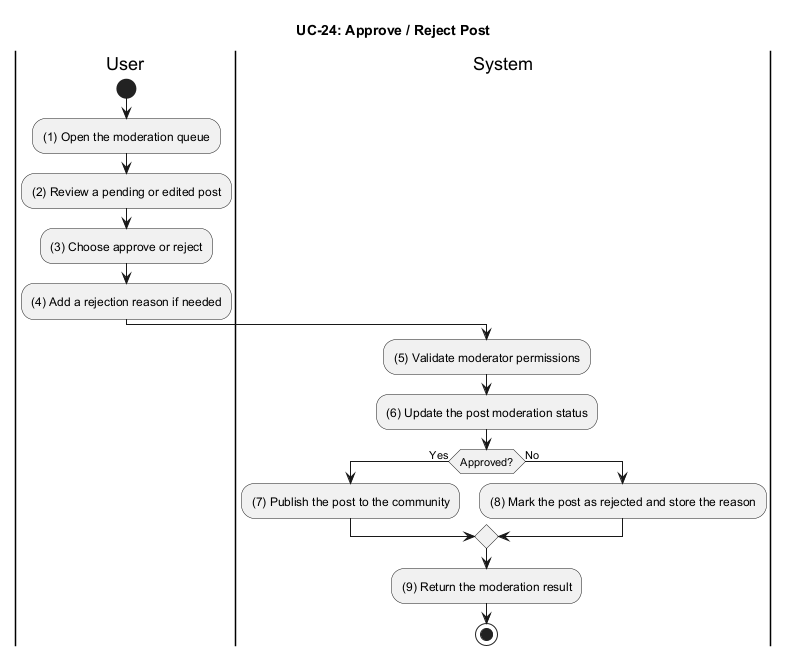
\includegraphics[width=0.8\textwidth]{./diagrams/activity_diagrams/UC_24_Approve_Reject_Post.png}
    \caption{Activity Diagram for UC-24}
    \label{fig:ad_uc24}
\end{figure}


\begin{longtblr}[
    caption = {Business Rules for UC-24 - Approve / Reject Post},
    label = {tab:uc24_business_rules}
]{
    width=\textwidth,
    hlines,
    vlines,
    rowhead = 1,
    rows = {valign=m, cmd=\nopagebreak},
    row{1} = {font=\bfseries, halign=c},
    colspec = {Q[c,1.8cm] Q[c,1.5cm] Q[c,3.0cm] Q[l,7.5cm]}
}
\textbf{ID} & \textbf{Activity} & \textbf{Rule Type} & \textbf{Description} \\

BR-UC24-01 & (5) & Authorization Rules &
\textbf{Open the Moderation Queue and Validate Moderator Permissions:}
\begin{itemize}
    \item The moderation queue endpoints require authentication.
    \item The service checks that the requester is a moderator of the target community before loading or moderating posts.
    \item if \textbf{authUser == null} or the user is not a moderator, then the system returns a forbidden response.
\end{itemize} \\

BR-UC24-02 & (2) & Workflow Rules &
\textbf{Load Pending or Edited Posts:}
\begin{itemize}
    \item The system loads pending posts with \textbf{\textit{GetPendingPosts()}}.
    \item The system loads edited posts with \textbf{\textit{GetEditedPosts()}}.
    \item The queued posts are filtered by community ID and moderation status before being returned.
\end{itemize} \\

BR-UC24-03 & (5) & Validation Rules &
\textbf{Validate the Moderation Decision:}
\begin{itemize}
    \item The controller binds the request to \texttt{ModeratePostRequest}.
    \item The request must include the community ID, post ID, and approve flag.
    \item if the moderation route parameters are missing or the request body is invalid, then the controller returns a bad request response.
\end{itemize} \\

BR-UC24-04 & (5) & Validation Rules &
\textbf{Validate the Target Post:}
\begin{itemize}
    \item The service loads the target post before applying the decision.
    \item The post must belong to the same community as the moderation request.
    \item The post must still be in \textbf{moderation\_status = pending}.
    \item if the post is missing, in another community, or not pending, then the operation stops with the corresponding error.
\end{itemize} \\

BR-UC24-05 & (7) & Workflow Rules &
\textbf{Approve the Post:}
\begin{itemize}
    \item if \textbf{approve = true}, then the service sets \textbf{moderation\_status = approved}.
    \item The service updates \textbf{moderated\_at} for the post.
    \item The service publishes a \texttt{PostApprovedEvent} so the post becomes visible to the community flow.
\end{itemize} \\

BR-UC24-06 & (8) & Workflow Rules &
\textbf{Reject the Post:}
\begin{itemize}
    \item if \textbf{approve = false}, then the service sets \textbf{moderation\_status = rejected}.
    \item The service stores a \texttt{ModerationResult} with \textbf{IsViolation = true} and the rejection reason.
    \item if no rejection reason is supplied, then the service uses the default moderator rejection reason.
    \item The service publishes a \texttt{PostRejectedEvent} for downstream notifications.
\end{itemize} \\

BR-UC24-07 & (9) & Message Rules &
\textbf{Return the Moderation Result:}
\begin{itemize}
    \item Moderator approval shall use \msgref{post-approved-success}; approval failures shall use \msgref{post-approve-failed}.
    \item Rejection or removal flows may reuse \msgref{delete-post-success} and \msgref{delete-post-failed} when the post is removed from the queue.
\end{itemize} \\

BR-UC24-08 & (9) & Message Rules &
\textbf{Return Moderation Error Message:}
\begin{itemize}
    \item Moderation failures shall return \errref{post-not-found}, \errref{forbidden}, \errref{community-not-found}, or \errref{invalid-id}.
\end{itemize} \\
\end{longtblr}



\subsection{UC-25 - Ban / Mute User}
\begin{table}[H]
\centering
\begin{tblr}{
    width=\textwidth,
    hlines,
    vlines,
    rows = {valign=m},
    colspec = {Q[l,3cm] Q[l,11cm]}
}
\textbf{Name} & Ban / Mute User \\
\textbf{Description} & This use case describes how a moderator restricts a user's participation in a community. \\
\textbf{Actor} & Moderator \\
\textbf{Trigger} & When the moderator chooses to ban or mute a user. \\
\textbf{Pre-condition} & The moderator is logged in to the system. \newline The target user belongs to the community. \\
\textbf{Post-condition} & The ban or mute restriction is stored. \newline The user is prevented from performing the restricted actions. \\
\end{tblr}
\caption{Use Case Specification - Ban / Mute User}
\end{table}


\begin{figure}[H]
    \centering
    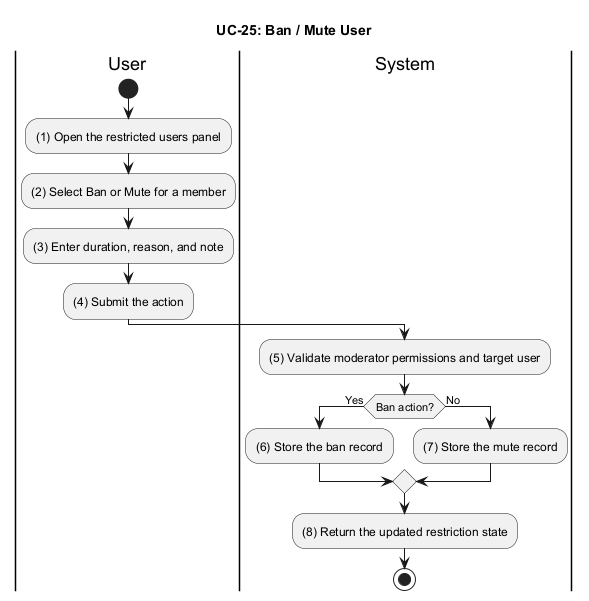
\includegraphics[width=0.8\textwidth]{./diagrams/activity_diagrams/UC_25_Ban_Mute_User.png}
    \caption{Activity Diagram for UC-25}
    \label{fig:ad_uc25}
\end{figure}


\begin{longtblr}[
    caption = {Business Rules for UC-25 - Ban / Mute User},
    label = {tab:uc25_business_rules}
]{
    width=\textwidth,
    hlines,
    vlines,
    rowhead = 1,
    rows = {valign=m, cmd=\nopagebreak},
    row{1} = {font=\bfseries, halign=c},
    colspec = {Q[c,1.8cm] Q[c,1.5cm] Q[c,3.0cm] Q[l,7.5cm]}
}
\textbf{ID} & \textbf{Activity} & \textbf{Rule Type} & \textbf{Description} \\

BR-UC25-01 & (5) & Authorization Rules &
\textbf{Open the Restricted Users Panel and Validate Moderator Access:}
\begin{itemize}
    \item The ban and mute actions require authentication.
    \item The service checks that the requester is a moderator of the target community.
    \item if \textbf{authUser == null} or the requester is not a moderator, then the system returns a forbidden response.
\end{itemize} \\

BR-UC25-02 & (5) & Validation Rules &
\textbf{Validate the Restriction Request:}
\begin{itemize}
    \item The system binds the request to \texttt{CommunityBanUserRequest}.
    \item The request must include \textbf{communityID}, \textbf{userID}, \textbf{type}, and \textbf{lengthDays}.
    \item The restriction type must be either \textbf{banned} or \textbf{muted}.
    \item The reason field is accepted by the API and is stored with the restriction record.
\end{itemize} \\

BR-UC25-03 & (5) & Validation Rules &
\textbf{Validate the Target User and Community:}
\begin{itemize}
    \item The service converts the community ID, user ID, and requester ID to object IDs.
    \item if any ID is invalid, then the operation stops with the corresponding error.
\end{itemize} \\

BR-UC25-04 & (6) & Workflow Rules &
\textbf{Store the Ban Record:}
\begin{itemize}
    \item if \textbf{type = banned}, then the service creates a \texttt{CommunityBan} record with \textbf{Type = banned}.
    \item The service calculates \textbf{ExpiresAt} from \textbf{lengthDays}.
    \item The repository clears any existing active restriction for the same user and community before inserting the new ban.
    \item The ban record stores the target user, community, reason, requester, banned time, expiration time, and soft-delete flags.
\end{itemize} \\

BR-UC25-05 & (7) & Workflow Rules &
\textbf{Store the Mute Record:}
\begin{itemize}
    \item if \textbf{type = muted}, then the service creates a \texttt{CommunityBan} record with \textbf{Type = muted}.
    \item The same expiration and audit fields are stored for mute actions.
    \item The repository clears any existing active restriction for the same user and community before inserting the new mute.
\end{itemize} \\

BR-UC25-06 & (8) & Message Rules &
\textbf{Return the Updated Restriction State:}
\begin{itemize}
    \item Restriction actions shall use \msgref{user-banned-success}, \msgref{user-muted-success}, \msgref{user-unbanned-success}, \msgref{user-unban-failed}, \msgref{user-unmuted-success}, or \msgref{user-unmute-failed} as applicable.
\end{itemize} \\

BR-UC25-07 & (8) & Message Rules &
\textbf{Return Restriction Error Message:}
\begin{itemize}
    \item Validation or authorization failures shall return \errref{user-not-found}, \errref{community-not-found}, \errref{membership-not-found}, \errref{forbidden}, or \errref{invalid-id}.
\end{itemize} \\
\end{longtblr}



\subsection{UC-26 - Configure Community}
\begin{table}[H]
\centering
\begin{tblr}{
    width=\textwidth,
    hlines,
    vlines,
    rows = {valign=m},
    colspec = {Q[l,3cm] Q[l,11cm]}
}
\textbf{Name} & Configure Community \\
\textbf{Description} & This use case describes how a community owner updates rules, privacy, and appearance settings. \\
\textbf{Actor} & Owner \\
\textbf{Trigger} & When the owner opens the community settings page and saves changes. \\
\textbf{Pre-condition} & The owner is logged in to the system. \newline The owner has permission to manage the community. \\
\textbf{Post-condition} & The community configuration is updated. \newline The new settings are applied to the community. \\
\end{tblr}
\caption{Use Case Specification - Configure Community}
\end{table}


\begin{figure}[H]
    \centering
    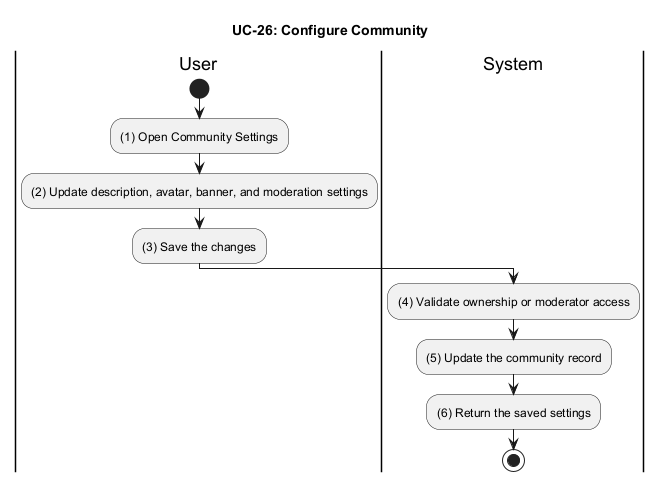
\includegraphics[width=0.8\textwidth]{./diagrams/activity_diagrams/UC_26_Configure_Community.png}
    \caption{Activity Diagram for UC-26}
    \label{fig:ad_uc26}
\end{figure}


\begin{longtblr}[
    caption = {Business Rules for UC-26 - Configure Community},
    label = {tab:uc26_business_rules}
]{
    width=\textwidth,
    hlines,
    vlines,
    rowhead = 1,
    rows = {valign=m, cmd=\nopagebreak},
    row{1} = {font=\bfseries, halign=c},
    colspec = {Q[c,1.8cm] Q[c,1.5cm] Q[c,3.0cm] Q[l,7.5cm]}
}
\textbf{ID} & \textbf{Activity} & \textbf{Rule Type} & \textbf{Description} \\

BR-UC26-01 & (4) & Authorization Rules &
\textbf{Open Community Settings and Validate Access:}
\begin{itemize}
    \item The community settings page requires a logged-in user.
    \item The service allows the update only when the requester is the community creator or an active moderator.
    \item if \textbf{authUser == null} or the requester lacks moderator access, then the system returns a forbidden response.
\end{itemize} \\

BR-UC26-02 & (4) & Validation Rules &
\textbf{Validate the Settings Request:}
\begin{itemize}
    \item The controller binds the request to \texttt{UpdateCommunityRequest}.
    \item The request must include the community ID.
    \item The request may include description, avatar, banner, moderation settings, and rules.
    \item if the payload cannot be bound, then the controller returns a bad request response.
\end{itemize} \\

BR-UC26-03 & (5) & Workflow Rules &
\textbf{Load the Community Record:}
\begin{itemize}
    \item The service loads the target community before applying changes.
    \item if the community does not exist, then the operation stops with the corresponding error.
\end{itemize} \\

BR-UC26-04 & (5) & Workflow Rules &
\textbf{Apply Community Field Updates:}
\begin{itemize}
    \item The service updates only the non-nil fields from the request.
    \item The configurable fields are description, avatar, banner, settings, and rules.
    \item The service rejects save attempts that do not change any field.
\end{itemize} \\

BR-UC26-05 & (5) & Constraint Rules &
\textbf{Require at Least One Change:}
\begin{itemize}
    \item if no update fields are provided, then the service returns \texttt{ErrNoFieldsToUpdate}.
\end{itemize} \\

BR-UC26-06 & (5) & Workflow Rules &
\textbf{Persist the Community Settings:}
\begin{itemize}
    \item The service saves the updated community through \textbf{\textit{UpdateCommunity()}}.
    \item The repository replaces the full community record after the in-memory updates are applied.
\end{itemize} \\

BR-UC26-07 & (6) & Message Rules &
\textbf{Return the Saved Community Settings:}
\begin{itemize}
    \item Successful community-configuration changes shall use \msgref{community-settings-saved}.
\end{itemize} \\

BR-UC26-08 & (6) & Message Rules &
\textbf{Return Community Update Error:}
\begin{itemize}
    \item Failed updates shall use \msgref{community-settings-save-failed}.
    \item Access or validation failures shall return \errref{community-not-found}, \errref{forbidden}, \errref{invalid-id}, or \errref{bad-request}.
\end{itemize} \\
\end{longtblr}


\subsection{UC-27 - Assign Roles}
\begin{table}[H]
\centering
\begin{tblr}{
    width=\textwidth,
    hlines,
    vlines,
    rows = {valign=m},
    colspec = {Q[l,3cm] Q[l,11cm]}
}
\textbf{Name} & Assign Roles \\
\textbf{Description} & This use case describes how a community owner appoints moderators or other roles for members. \\
\textbf{Actor} & Owner \\
\textbf{Trigger} & When the owner invites or activates a role for another member. \\
\textbf{Pre-condition} & The owner is logged in to the system. \newline The target member belongs to the community. \\
\textbf{Post-condition} & The role assignment is stored successfully. \newline The target member gains the new permissions. \\
\end{tblr}
\caption{Use Case Specification - Assign Roles}
\end{table}


\begin{figure}[H]
    \centering
    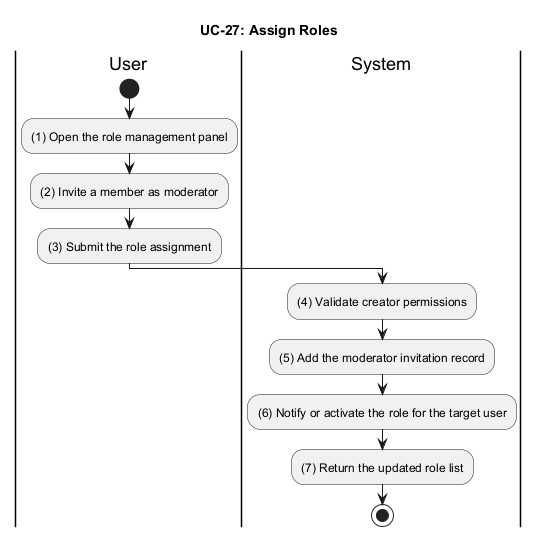
\includegraphics[width=0.7\textwidth]{./diagrams/activity_diagrams/UC_27_Assign_Roles.png}
    \caption{Activity Diagram for UC-27}
    \label{fig:ad_uc27}
\end{figure}


\begin{longtblr}[
    caption = {Business Rules for UC-27 - Assign Roles},
    label = {tab:uc27_business_rules}
]{
    width=\textwidth,
    hlines,
    vlines,
    rowhead = 1,
    rows = {valign=m, cmd=\nopagebreak},
    row{1} = {font=\bfseries, halign=c},
    colspec = {Q[c,1.8cm] Q[c,1.5cm] Q[c,3.0cm] Q[l,7.5cm]}
}
\textbf{ID} & \textbf{Activity} & \textbf{Rule Type} & \textbf{Description} \\

BR-UC27-01 & (4) & Authorization Rules &
\textbf{Open the Role Management Panel and Validate Creator Access:}
\begin{itemize}
    \item The role assignment actions require authentication.
    \item The service allows adding moderators only when the requester is the community creator.
    \item The target user must be invited from the creator's community role management flow.
    \item if \textbf{authUser == null} or the requester is not the creator, then the system returns a forbidden response.
\end{itemize} \\

BR-UC27-02 & (4) & Validation Rules &
\textbf{Validate the Moderator Invitation Request:}
\begin{itemize}
    \item The controller binds the request to \texttt{AddModeratorRequest}.
    \item The request must include the community ID and at least one moderator user ID.
    \item The target user IDs are resolved from the invited usernames in the current UI flow.
    \item if the request payload cannot be bound or contains no target users, then the controller returns a bad request response.
\end{itemize} \\

BR-UC27-03 & (5) & Constraint Rules &
\textbf{Prevent Duplicate Active Moderators:}
\begin{itemize}
    \item The service rejects a user who is already an active moderator.
    \item Existing inactive invitations for the same user are removed before a new invite is stored.
    \item if the moderator already exists as active, then the service returns \texttt{ErrModeratorAlreadyExists}.
\end{itemize} \\

BR-UC27-04 & (5) & Workflow Rules &
\textbf{Add the Moderator Invitation Record:}
\begin{itemize}
    \item The service loads the community and the invited user before storing the role change.
    \item The service creates a \texttt{Moderator} entry with \textbf{IsActive = false} and the current assignment time.
    \item The community record is replaced after the invitation is appended.
    \item The service publishes a \texttt{ModeratorAddedEvent} after persistence succeeds.
\end{itemize} \\

BR-UC27-05 & (6) & Workflow Rules &
\textbf{Activate the Moderator Role:}
\begin{itemize}
    \item The invited user can activate the moderator role through the activation endpoint.
    \item The repository marks the matching moderator entry as active and refreshes the assignment timestamp.
    \item if the invitation cannot be matched, then the repository returns a bad request error.
\end{itemize} \\

BR-UC27-06 & (7) & Message Rules &
\textbf{Return the Updated Role List:}
\begin{itemize}
    \item Role-assignment feedback shall use \msgref{add-moderator-success} on success and \msgref{add-moderator-failed} on failure.
\end{itemize} \\

BR-UC27-07 & (7) & Message Rules &
\textbf{Return Role Assignment Error:}
\begin{itemize}
    \item Validation failures shall return \errref{user-not-found}, \errref{community-not-found}, \errref{moderator-already-exists}, \errref{user-not-member}, \errref{cannot-remove-moderator}, \errref{cannot-remove-creator}, or \errref{invalid-id}.
\end{itemize} \\
\end{longtblr}



\subsection{UC-28 - Handle Global Reports}
\begin{table}[H]
\centering
\begin{tblr}{
    width=\textwidth,
    hlines,
    vlines,
    rows = {valign=m},
    colspec = {Q[l,3cm] Q[l,11cm]}
}
\textbf{Name} & Handle Global Reports \\
\textbf{Description} & This use case describes how a system admin reviews and acts on platform-wide violation reports. \\
\textbf{Actor} & System Admin \\
\textbf{Trigger} & When the admin opens the global reports dashboard. \\
\textbf{Pre-condition} & The admin is logged in to the system. \newline There are reports available for review. \\
\textbf{Post-condition} & The selected reports are reviewed or deleted. \newline The report queue is updated. \\
\end{tblr}
\caption{Use Case Specification - Handle Global Reports}
\end{table}


\begin{figure}[H]
    \centering
    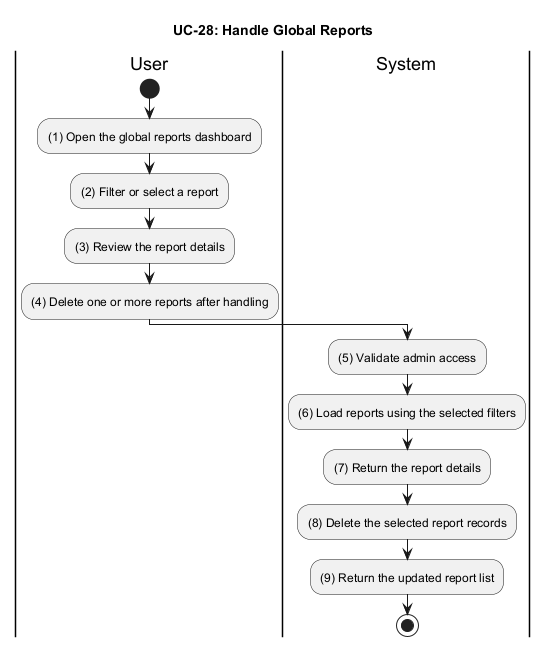
\includegraphics[width=0.9\textwidth]{./diagrams/activity_diagrams/UC_28_Handle_Global_Reports.png}
    \caption{Activity Diagram for UC-28}
    \label{fig:ad_uc28}
\end{figure}


\begin{longtblr}[
    caption = {Business Rules for UC-28 - Handle Global Reports},
    label = {tab:uc28_business_rules}
]{
    width=\textwidth,
    hlines,
    vlines,
    rowhead = 1,
    rows = {valign=m, cmd=\nopagebreak},
    row{1} = {font=\bfseries, halign=c},
    colspec = {Q[c,1.8cm] Q[c,1.5cm] Q[c,3.0cm] Q[l,7.5cm]}
}
\textbf{ID} & \textbf{Activity} & \textbf{Rule Type} & \textbf{Description} \\

BR-UC28-01 & (5) & Authorization Rules &
\textbf{Open the Global Reports Dashboard and Validate Admin Access:}
\begin{itemize}
    \item The global reports routes require authentication and admin privileges.
    \item if the requester is not an admin, then the system returns a forbidden response.
    \item The dashboard and report detail actions are only available through the admin reports routes.
\end{itemize} \\

BR-UC28-02 & (6) & Validation Rules &
\textbf{Validate the Report Filter Request:}
\begin{itemize}
    \item The system binds the query to \texttt{GetReportsFilterQuery}.
    \item The request may include reporter ID, target ID, target type, reason, date range, page, and page size.
    \item if the query cannot be bound, then the controller returns a bad request response.
\end{itemize} \\

BR-UC28-03 & (7) & Workflow Rules &
\textbf{Load Report Details and Filtered Results:}
\begin{itemize}
    \item The service loads reports using \textbf{\textit{GetReportsFilter()}}.
    \item The admin can open a single report using \textbf{\textit{GetReportByIDAdmin()}}.
\end{itemize} \\

BR-UC28-04 & (8) & Validation Rules &
\textbf{Validate Selected Report IDs for Deletion:}
\begin{itemize}
    \item The controller binds batch deletion requests to \texttt{DeleteReportsRequest}.
    \item The request must contain at least one report ID.
    \item if the batch list is empty or the request is invalid, then the controller returns a bad request response.
\end{itemize} \\

BR-UC28-05 & (8) & Workflow Rules &
\textbf{Delete Single or Multiple Reports:}
\begin{itemize}
    \item The admin can delete one report using \textbf{\textit{DeleteReportByIDAdmin()}}.
    \item The admin can delete multiple reports using \textbf{\textit{DeleteReportsByIDAdmin()}}.
    \item The service deletes the selected report records after validation succeeds.
\end{itemize} \\

BR-UC28-06 & (9) & Message Rules &
\textbf{Return the Updated Report List:}
\begin{itemize}
    \item Report-administration UI feedback shall use \msgref{reports-load-failed}, \msgref{confirm-delete-report}, \msgref{delete-report-success}, or \msgref{delete-report-failed}.
\end{itemize} \\

BR-UC28-07 & (9) & Message Rules &
\textbf{Return Report Management Error:}
\begin{itemize}
    \item Administrative failures shall return \errref{admin-access-required}, \errref{report-not-found}, \errref{invalid-id}, \errref{bad-request}, or \errref{forbidden}.
\end{itemize} \\
\end{longtblr}



\subsection{UC-29 - Manage Platform}
\begin{table}[H]
\centering
\begin{tblr}{
    width=\textwidth,
    hlines,
    vlines,
    rows = {valign=m},
    colspec = {Q[l,3cm] Q[l,11cm]}
}
\textbf{Name} & Manage Platform \\
\textbf{Description} & This use case describes how a system admin manages users and communities globally. \\
\textbf{Actor} & System Admin \\
\textbf{Trigger} & When the admin opens the platform management area and selects a target entity. \\
\textbf{Pre-condition} & The admin is logged in to the system. \newline The admin has global management privileges. \\
\textbf{Post-condition} & The selected user or community is banned or unbanned. \newline The platform state is updated accordingly. \\
\end{tblr}
\caption{Use Case Specification - Manage Platform}
\end{table}


\begin{figure}[H]
    \centering
    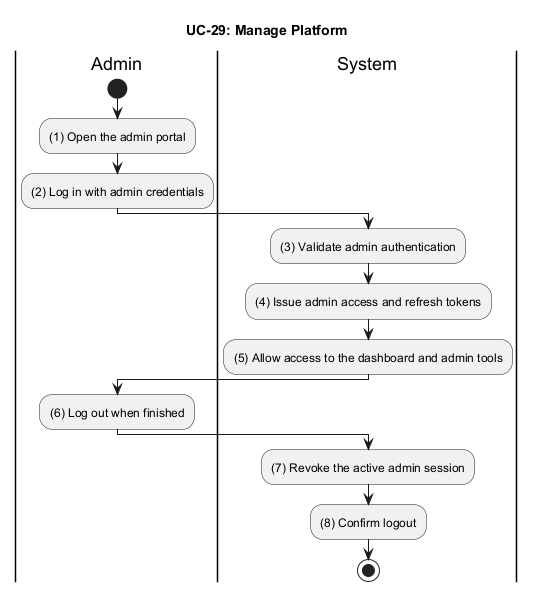
\includegraphics[width=0.9\textwidth]{./diagrams/activity_diagrams/UC_29_Manage_Platform.png}
    \caption{Activity Diagram for UC-29}
    \label{fig:ad_uc29}
\end{figure}


\begin{longtblr}[
    caption = {Business Rules for UC-29 - Manage Platform},
    label = {tab:uc29_business_rules}
]{
    width=\textwidth,
    hlines,
    vlines,
    rowhead = 1,
    rows = {valign=m, cmd=\nopagebreak},
    row{1} = {font=\bfseries, halign=c},
    colspec = {Q[c,1.8cm] Q[c,1.5cm] Q[c,3.0cm] Q[l,7.5cm]}
}
\textbf{ID} & \textbf{Activity} & \textbf{Rule Type} & \textbf{Description} \\

BR-UC29-01 & (3) & Authorization Rules &
\textbf{Validate Admin Login and Access Rights:}
\begin{itemize}
    \item The login endpoint accepts an identifier and password.
    \item The service loads the account by email or username and requires the \texttt{admin} role.
    \item The service rejects banned, deleted, or non-admin accounts before issuing tokens.
    \item The service verifies the password for local accounts in \textbf{\textit{AdminLogin()}}.
\end{itemize} \\

BR-UC29-02 & (3) & Validation Rules &
\textbf{Validate the Admin Login Request:}
\begin{itemize}
    \item The system binds the login payload to \texttt{UserLoginRequest}.
    \item The request must include both identifier and password fields.
    \item if the payload cannot be bound, then the system returns a bad request response.
    \item if the credentials are invalid, then the service returns an invalid credentials response.
\end{itemize} \\

BR-UC29-03 & (3--5) & Workflow Rules &
\textbf{Issue Admin Tokens and Allow Protected Access:}
\begin{itemize}
    \item The service generates access and refresh tokens with \textbf{\textit{AdminLogin()}} after successful authentication.
    \item The login system returns the authenticated user together with both tokens.
    \item Admin dashboard and tool routes require \texttt{RequireAuth()} and \texttt{RequireAdmin()} before they can be reached.
    \item The protected admin stats routes expose the dashboard overview and related admin tools only after the token is accepted.
\end{itemize} \\

BR-UC29-04 & (7) & Workflow Rules &
\textbf{Revoke the Active Admin Session:}
\begin{itemize}
    \item The logout endpoint reads the bearer access token and optional refresh token from the request.
    \item The service extracts the token JTIs and invalidates them when token revocation is available in \textbf{\textit{AdminLogout()}}.
    \item The logout call completes even when token invalidation is unavailable, so the admin session ends cleanly.
\end{itemize} \\

BR-UC29-05 & (8) & Message Rules &
\textbf{Return the Admin Auth Result:}
\begin{itemize}
    \item Successful admin sign-in shall use \msgref{login-successful}; logout completion has no dedicated message code in the current code.
    \item Authentication and access failures shall return \errref{invalid-credentials}, \errref{admin-access-required}, \errref{invalid-token}, \errref{user-inactive}, or \errref{user-not-found}.
\end{itemize} \\
\end{longtblr}



\subsection{UC-30 - View Analytics}
\begin{table}[H]
\centering
\begin{tblr}{
    width=\textwidth,
    hlines,
    vlines,
    rows = {valign=m},
    colspec = {Q[l,3cm] Q[l,11cm]}
}
\textbf{Name} & View Analytics \\
\textbf{Description} & This use case describes how a system admin reviews platform usage and performance metrics. \\
\textbf{Actor} & System Admin \\
\textbf{Trigger} & When the admin opens the analytics dashboard. \\
\textbf{Pre-condition} & The admin is logged in to the system. \newline Analytics data is available for the selected period. \\
\textbf{Post-condition} & The analytics dashboard is displayed with current metrics. \newline The admin can review user, content, and moderation statistics. \\
\end{tblr}
\caption{Use Case Specification - View Analytics}
\end{table}


\begin{figure}[H]
    \centering
    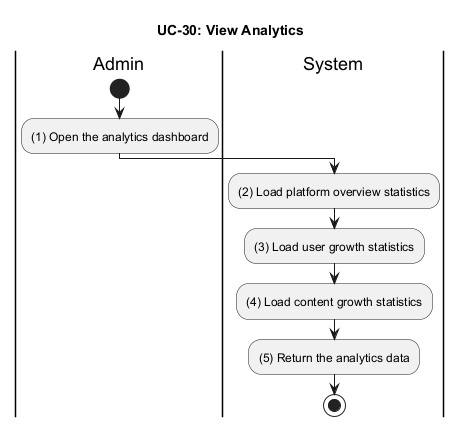
\includegraphics[width=0.8\textwidth]{./diagrams/activity_diagrams/UC_30_View_Analytics.png}
    \caption{Activity Diagram for UC-30}
    \label{fig:ad_uc30}
\end{figure}


\begin{longtblr}[
    caption = {Business Rules for UC-30 - View Analytics},
    label = {tab:uc30_business_rules}
]{
    width=\textwidth,
    hlines,
    vlines,
    rowhead = 1,
    rows = {valign=m, cmd=\nopagebreak},
    row{1} = {font=\bfseries, halign=c},
    colspec = {Q[c,1.8cm] Q[c,1.5cm] Q[c,3.0cm] Q[l,7.5cm]}
}
\textbf{ID} & \textbf{Activity} & \textbf{Rule Type} & \textbf{Description} \\

BR-UC30-01 & (2) & Authorization Rules &
\textbf{Open the Analytics Dashboard with Admin Access:}
\begin{itemize}
    \item The analytics routes require authentication and the \texttt{admin} role.
    \item The protected admin stats routes are guarded by \texttt{RequireAuth()} and \texttt{RequireAdmin()}.
    \item if the requester is not an admin, then the system returns a forbidden response.
\end{itemize} \\

BR-UC30-02 & (2) & Validation Rules &
\textbf{Validate the Analytics Query Parameters:}
\begin{itemize}
    \item The controller binds the user statistics query to \texttt{GetUserStatsQuery}.
    \item The controller binds the content statistics query to \texttt{GetContentStatsQuery}.
    \item The \texttt{period} field is optional and defaults to \texttt{week} when omitted.
    \item if the query cannot be bound, then the controller returns a bad request response.
\end{itemize} \\

BR-UC30-03 & (2) & Workflow Rules &
\textbf{Load the Platform Overview Snapshot:}
\begin{itemize}
    \item The service loads the platform overview using \textbf{\textit{GetPlatformOverview()}}.
    \item The overview aggregates user, community, content, and moderation statistics from the repositories.
    \item The overview response includes the current snapshot timestamp in \texttt{UpdatedAt}.
\end{itemize} \\

BR-UC30-04 & (3--5) & Workflow Rules &
\textbf{Load User and Content Growth Statistics:}
\begin{itemize}
    \item The service loads user statistics using \textbf{\textit{GetUserStats()}} and content statistics using \textbf{\textit{GetContentStats()}}.
    \item The service selects the growth window from the requested period and falls back to \texttt{week} when needed.
    \item The response includes the overview and the corresponding growth series for the requested analytics view.
\end{itemize} \\

BR-UC30-05 & (5) & Message Rules &
\textbf{Return the Analytics Result or Error:}
\begin{itemize}
    \item Analytics loading failures shall use \msgref{analytics-load-failed}.
    \item Successful analytics requests return dashboard data inline and do not define a dedicated success toast in the current code.
    \item Access failures shall return \errref{admin-access-required}, \errref{not-authenticated}, \errref{invalid-token}, or \errref{forbidden}.
\end{itemize} \\
\end{longtblr}


\section{Data Requirements}

\subsection{Logical Data Model}

\begin{figure}[H]
    \centering
    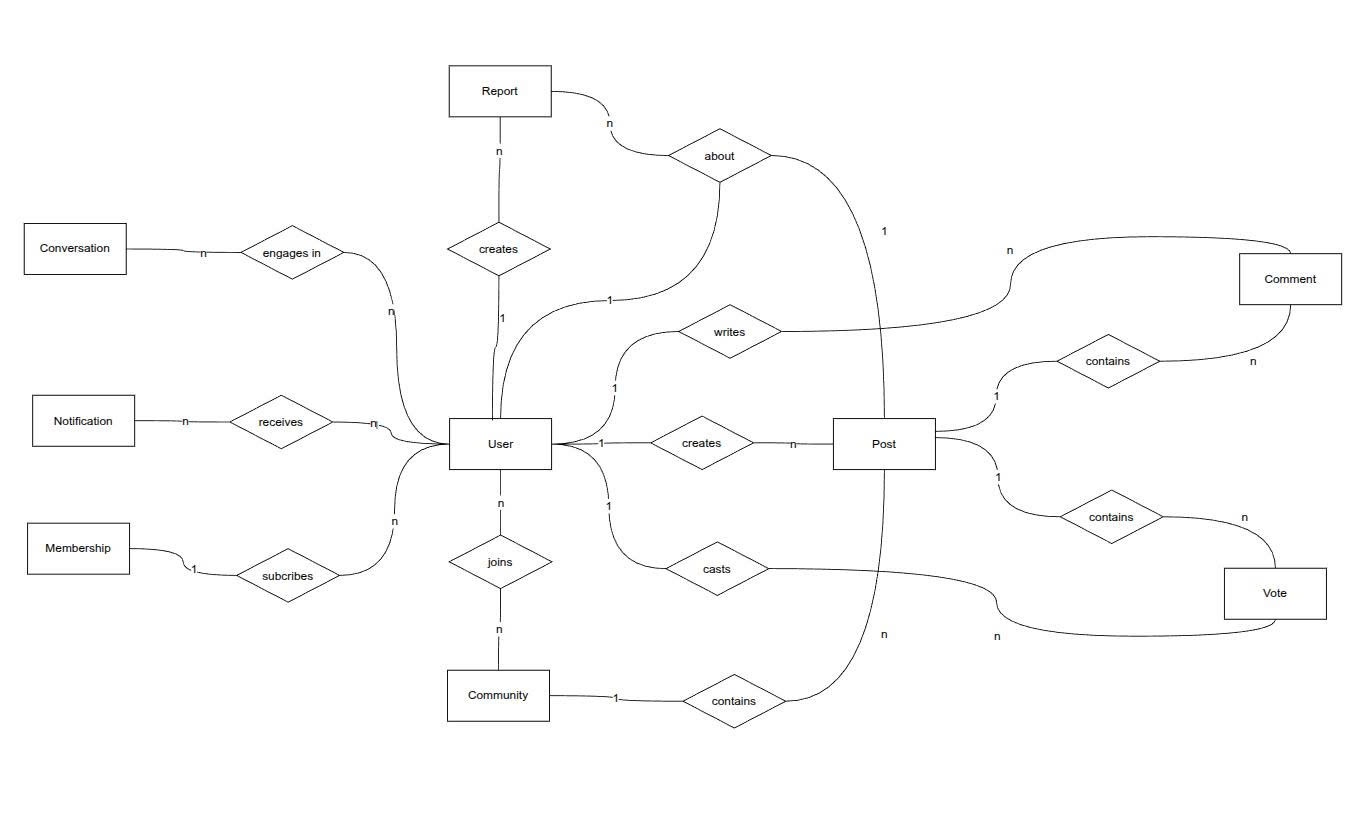
\includegraphics[width=\textwidth]{./diagrams/Partial data model for LKForum.jpg}
    \caption{Logical Data Model for LKForum}
    \label{fig:data_model_lkforum}
\end{figure}

\subsection{Data Dictionary}

\subsubsection{Authentication and User Profile Models}

\begin{longtblr}[
    caption = {User},
    label = {tab:data_dictionary_user}
]{
    width=\textwidth,
    hlines,
    vlines,
    rowhead = 1,
    rows = {valign=m, cmd=\nopagebreak},
    row{1} = {font=\bfseries, halign=c},
    colspec = {Q[l,2.8cm] Q[l,4.5cm] Q[c,2.5cm] Q[c,1.5cm] Q[l,4.2cm]}
}
\textbf{Data Element} & \textbf{Description} & \textbf{Composition / Data Type} & \textbf{Length} & \textbf{Values} \\

ID & Unique identifier of a user. & objectId & 24 & System-generated, unique. \\
Username & Display name used to identify a user account. & string & -- & Must be unique within the platform. \\
Email & Email address used for authentication and contact. & string & -- & Must be unique and valid. \\
Reputation & User reputation score. & integer & -- & System-maintained counter. \\
Password & Hashed password for a local account. & string & -- & Stored only for local providers. \\
Provider & Authentication source for a user account. & enum & -- & local, google \\
ProviderID & External account identifier returned by the provider. & string & -- & Used for third-party login linkage. \\
Role & Platform-wide role of the user. & enum & -- & user, admin \\
RoleContent & Role-specific data attached to the user account. & object & -- & Contains user or admin sub-document data. \\
Settings & User preference configuration. & object & -- & Contains appearance, notification, privacy, and content settings. \\
IsVerified & Indicates whether the account has been verified. & boolean & -- & true, false \\
IsBanned & Indicates whether the account is currently banned. & boolean & -- & true, false \\
BanUntil & Timestamp when a ban expires, if any. & timestamp & -- & Null means permanent ban. \\
BanReason & Reason recorded for a ban action. & string & -- & Optional free text. \\
CreatedAt & Timestamp when the record was created. & timestamp & -- & System-generated. \\
DeletedAt & Timestamp for soft-deleted records. & timestamp & -- & Null when not deleted. \\
\end{longtblr}

\begin{longtblr}[
    caption = {RoleContent},
    label = {tab:data_dictionary_role_content}
]{
    width=\textwidth,
    hlines,
    vlines,
    rowhead = 1,
    rows = {valign=m, cmd=\nopagebreak},
    row{1} = {font=\bfseries, halign=c},
    colspec = {Q[l,2.8cm] Q[l,4.5cm] Q[c,2.5cm] Q[c,1.5cm] Q[l,4.2cm]}
}
\textbf{Data Element} & \textbf{Description} & \textbf{Composition / Data Type} & \textbf{Length} & \textbf{Values} \\

AsUser & User-specific profile data. & object & -- & See UserRoleContent table. \\
AsAdmin & Admin-specific profile data. & object & -- & See AdminRoleContent table. \\
\end{longtblr}

\begin{longtblr}[
    caption = {UserRoleContent},
    label = {tab:data_dictionary_user_role_content}
]{
    width=\textwidth,
    hlines,
    vlines,
    rowhead = 1,
    rows = {valign=m, cmd=\nopagebreak},
    row{1} = {font=\bfseries, halign=c},
    colspec = {Q[l,2.8cm] Q[l,4.5cm] Q[c,2.5cm] Q[c,1.5cm] Q[l,4.2cm]}
}
\textbf{Data Element} & \textbf{Description} & \textbf{Composition / Data Type} & \textbf{Length} & \textbf{Values} \\

Avatar & Profile image. & object & -- & See Image table. \\
Cover & Cover image. & object & -- & See Image table. \\
Bio & Short biography. & string & -- & User-generated text. \\
Gender & Declared gender. & enum & -- & male, female, prefer_not_to_say \\
DateOfBirth & User date of birth. & timestamp & -- & Optional date value. \\
Location & Province or city. & enum & -- & One of the provinces defined in model/location.go. \\
Interests & List of user interests. & array[string] & -- & Values defined in model/interest.go. \\
SocialLinks & Collection of public social profiles. & object & -- & Website, Facebook, YouTube, GitHub links. \\
Stats & User activity statistics. & object & -- & Post, comment, and vote counters plus timestamps. \\
\end{longtblr}

\begin{longtblr}[
    caption = {SocialLinks},
    label = {tab:data_dictionary_social_links}
]{
    width=\textwidth,
    hlines,
    vlines,
    rowhead = 1,
    rows = {valign=m, cmd=\nopagebreak},
    row{1} = {font=\bfseries, halign=c},
    colspec = {Q[l,2.8cm] Q[l,4.5cm] Q[c,2.5cm] Q[c,1.5cm] Q[l,4.2cm]}
}
\textbf{Data Element} & \textbf{Description} & \textbf{Composition / Data Type} & \textbf{Length} & \textbf{Values} \\

Website & Personal website URL. & string & -- & Optional URL. \\
Facebook & Facebook profile URL. & string & -- & Optional URL. \\
YouTube & YouTube channel URL. & string & -- & Optional URL. \\
GitHub & GitHub profile URL. & string & -- & Optional URL. \\
\end{longtblr}

\begin{longtblr}[
    caption = {ActivityStats},
    label = {tab:data_dictionary_activity_stats}
]{
    width=\textwidth,
    hlines,
    vlines,
    rowhead = 1,
    rows = {valign=m, cmd=\nopagebreak},
    row{1} = {font=\bfseries, halign=c},
    colspec = {Q[l,2.8cm] Q[l,4.5cm] Q[c,2.5cm] Q[c,1.5cm] Q[l,4.2cm]}
}
\textbf{Data Element} & \textbf{Description} & \textbf{Composition / Data Type} & \textbf{Length} & \textbf{Values} \\

PostCount & Number of posts created. & integer & -- & System-maintained counter. \\
CommentCount & Number of comments created. & integer & -- & System-maintained counter. \\
TotalUpvotes & Total upvotes received. & integer & -- & System-maintained counter. \\
JoinedAt & Timestamp when the user joined. & timestamp & -- & System-generated. \\
LastActiveAt & Timestamp of the last activity. & timestamp & -- & System-generated. \\
\end{longtblr}

\begin{longtblr}[
    caption = {AdminRoleContent},
    label = {tab:data_dictionary_admin_role_content}
]{
    width=\textwidth,
    hlines,
    vlines,
    rowhead = 1,
    rows = {valign=m, cmd=\nopagebreak},
    row{1} = {font=\bfseries, halign=c},
    colspec = {Q[l,2.8cm] Q[l,4.5cm] Q[c,2.5cm] Q[c,1.5cm] Q[l,4.2cm]}
}
\textbf{Data Element} & \textbf{Description} & \textbf{Composition / Data Type} & \textbf{Length} & \textbf{Values} \\

Permissions & Admin capability list. & array[string] & -- & Permission names granted to the admin. \\
\end{longtblr}

\begin{longtblr}[
    caption = {UserSettings},
    label = {tab:data_dictionary_user_settings}
]{
    width=\textwidth,
    hlines,
    vlines,
    rowhead = 1,
    rows = {valign=m, cmd=\nopagebreak},
    row{1} = {font=\bfseries, halign=c},
    colspec = {Q[l,2.8cm] Q[l,4.5cm] Q[c,2.5cm] Q[c,1.5cm] Q[l,4.2cm]}
}
\textbf{Data Element} & \textbf{Description} & \textbf{Composition / Data Type} & \textbf{Length} & \textbf{Values} \\

Appearance & Visual preferences. & object & -- & See AppearanceSettings table. \\
Notifications & Notification preferences. & object & -- & See NotificationSettings table. \\
Privacy & Privacy preferences. & object & -- & See PrivacySettings table. \\
Content & Content filtering preferences. & object & -- & See ContentSettings table. \\
\end{longtblr}

\begin{longtblr}[
    caption = {AppearanceSettings},
    label = {tab:data_dictionary_appearance_settings}
]{
    width=\textwidth,
    hlines,
    vlines,
    rowhead = 1,
    rows = {valign=m, cmd=\nopagebreak},
    row{1} = {font=\bfseries, halign=c},
    colspec = {Q[l,2.8cm] Q[l,4.5cm] Q[c,2.5cm] Q[c,1.5cm] Q[l,4.2cm]}
}
\textbf{Data Element} & \textbf{Description} & \textbf{Composition / Data Type} & \textbf{Length} & \textbf{Values} \\

Theme & UI theme preference. & enum & -- & light, dark, auto \\
FontSize & UI font size preference. & enum & -- & small, medium, large \\
\end{longtblr}

\begin{longtblr}[
    caption = {NotificationSettings},
    label = {tab:data_dictionary_notification_settings}
]{
    width=\textwidth,
    hlines,
    vlines,
    rowhead = 1,
    rows = {valign=m, cmd=\nopagebreak},
    row{1} = {font=\bfseries, halign=c},
    colspec = {Q[l,2.8cm] Q[l,4.5cm] Q[c,2.5cm] Q[c,1.5cm] Q[l,4.2cm]}
}
\textbf{Data Element} & \textbf{Description} & \textbf{Composition / Data Type} & \textbf{Length} & \textbf{Values} \\

InAppEnabled & In-app notification toggle. & boolean & -- & true, false \\
EmailEnabled & Email notification toggle. & boolean & -- & true, false \\
NotifyOn-Comment & Notify on comments. & boolean & -- & true, false \\
NotifyOn-Mention & Notify on mentions. & boolean & -- & true, false \\
NotifyOnUpvote & Notify on upvotes. & boolean & -- & true, false \\
NotifyOnMessage & Notify on private messages. & boolean & -- & true, false \\
\end{longtblr}

\begin{longtblr}[
    caption = {PrivacySettings},
    label = {tab:data_dictionary_privacy_settings}
]{
    width=\textwidth,
    hlines,
    vlines,
    rowhead = 1,
    rows = {valign=m, cmd=\nopagebreak},
    row{1} = {font=\bfseries, halign=c},
    colspec = {Q[l,2.8cm] Q[l,4.5cm] Q[c,2.5cm] Q[c,1.5cm] Q[l,4.2cm]}
}
\textbf{Data Element} & \textbf{Description} & \textbf{Composition / Data Type} & \textbf{Length} & \textbf{Values} \\

ShowProfile & Controls whether a profile is public. & boolean & -- & true, false \\
ShowEmail & Controls whether email is visible on the profile. & boolean & -- & true, false \\
ShowPostHistory & Controls whether post history is visible. & boolean & -- & true, false \\
AllowDirect-Messages & Controls whether direct messages are allowed. & boolean & -- & true, false \\
AllowMentions & Controls whether mentions are allowed. & boolean & -- & true, false \\
\end{longtblr}

\begin{longtblr}[
    caption = {ContentSettings},
    label = {tab:data_dictionary_content_settings}
]{
    width=\textwidth,
    hlines,
    vlines,
    rowhead = 1,
    rows = {valign=m, cmd=\nopagebreak},
    row{1} = {font=\bfseries, halign=c},
    colspec = {Q[l,2.8cm] Q[l,4.5cm] Q[c,2.5cm] Q[c,1.5cm] Q[l,4.2cm]}
}
\textbf{Data Element} & \textbf{Description} & \textbf{Composition / Data Type} & \textbf{Length} & \textbf{Values} \\

AllowNSFW & Controls whether NSFW content is allowed. & boolean & -- & true, false \\
\end{longtblr}

\begin{longtblr}[
    caption = {Verification Records},
    label = {tab:data_dictionary_verification}
]{
    width=\textwidth,
    hlines,
    vlines,
    rowhead = 1,
    rows = {valign=m, cmd=\nopagebreak},
    row{1} = {font=\bfseries, halign=c},
    colspec = {Q[l,2.8cm] Q[l,4.5cm] Q[c,2.5cm] Q[c,1.5cm] Q[l,4.2cm]}
}
\textbf{Data Element} & \textbf{Description} & \textbf{Composition / Data Type} & \textbf{Length} & \textbf{Values} \\

EmailVerification-.ID & Unique identifier of an email verification record. & objectId & 24 & System-generated, unique. \\
EmailVerification-.Email & Email being verified. & string & -- & Must be unique and valid. \\
EmailVerification-.OTP & One-time password used for verification. & string & 6 & Six-digit numeric code. \\
EmailVerification-.OTPExpiresAt & Expiration timestamp for the OTP. & timestamp & -- & System-generated. \\
EmailVerification-.IsVerified & Indicates whether the OTP has already been verified. & boolean & -- & true, false \\
EmailVerification-.Nonce & Anti-replay token. & string & -- & System-generated random value. \\
EmailVerification-.CreatedAt & Timestamp when the record was created. & timestamp & -- & System-generated. \\
\end{longtblr}

\begin{longtblr}[
    caption = {PasswordReset},
    label = {tab:data_dictionary_password_reset}
]{
    width=\textwidth,
    hlines,
    vlines,
    rowhead = 1,
    rows = {valign=m, cmd=\nopagebreak},
    row{1} = {font=\bfseries, halign=c},
    colspec = {Q[l,2.8cm] Q[l,4.5cm] Q[c,2.5cm] Q[c,1.5cm] Q[l,4.2cm]}
}
\textbf{Data Element} & \textbf{Description} & \textbf{Composition / Data Type} & \textbf{Length} & \textbf{Values} \\

PasswordReset-.ID & Unique identifier of a password reset record. & objectId & 24 & System-generated, unique. \\
PasswordReset-.Email & Email being reset. & string & -- & Must be unique and valid. \\
PasswordReset-.OTP & One-time password used for reset. & string & 6 & Six-digit numeric code. \\
PasswordReset-.OTPExpiresAt & Expiration timestamp for the OTP. & timestamp & -- & System-generated. \\
PasswordReset-.IsVerified & Indicates whether the OTP has already been verified. & boolean & -- & true, false \\
PasswordReset-.Nonce & Anti-replay token. & string & -- & System-generated random value. \\
PasswordReset-.CreatedAt & Timestamp when the record was created. & timestamp & -- & System-generated. \\
\end{longtblr}

\begin{longtblr}[
    caption = {Image},
    label = {tab:data_dictionary_image}
]{
    width=\textwidth,
    hlines,
    vlines,
    rowhead = 1,
    rows = {valign=m, cmd=\nopagebreak},
    row{1} = {font=\bfseries, halign=c},
    colspec = {Q[l,2.8cm] Q[l,4.5cm] Q[c,2.5cm] Q[c,1.5cm] Q[l,4.2cm]}
}
\textbf{Data Element} & \textbf{Description} & \textbf{Composition / Data Type} & \textbf{Length} & \textbf{Values} \\

URL & Public URL of a stored image. & string & -- & Cloudinary or equivalent media URL. \\
PublicID & Provider-specific image identifier. & string & -- & Used for delete/update operations. \\
UploadedAt & Timestamp when the image was uploaded. & timestamp & -- & System-generated. \\
\end{longtblr}

\begin{longtblr}[
    caption = {Video},
    label = {tab:data_dictionary_video}
]{
    width=\textwidth,
    hlines,
    vlines,
    rowhead = 1,
    rows = {valign=m, cmd=\nopagebreak},
    row{1} = {font=\bfseries, halign=c},
    colspec = {Q[l,2.8cm] Q[l,4.5cm] Q[c,2.5cm] Q[c,1.5cm] Q[l,4.2cm]}
}
\textbf{Data Element} & \textbf{Description} & \textbf{Composition / Data Type} & \textbf{Length} & \textbf{Values} \\

URL & Public URL of a stored video. & string & -- & Cloudinary or equivalent media URL. \\
PublicID & Provider-specific video identifier. & string & -- & Used for delete/update operations. \\
UploadedAt & Timestamp when the video was uploaded. & timestamp & -- & System-generated. \\
\end{longtblr}

\subsubsection{Community and Membership Models}

\begin{longtblr}[
    caption = {Community},
    label = {tab:data_dictionary_community}
]{
    width=\textwidth,
    hlines,
    vlines,
    rowhead = 1,
    rows = {valign=m, cmd=\nopagebreak},
    row{1} = {font=\bfseries, halign=c},
    colspec = {Q[l,2.8cm] Q[l,4.5cm] Q[c,2.5cm] Q[c,1.5cm] Q[l,4.2cm]}
}
\textbf{Data Element} & \textbf{Description} & \textbf{Composition / Data Type} & \textbf{Length} & \textbf{Values} \\

ID & Unique identifier of a community. & objectId & 24 & System-generated, unique. \\
Name & Public name of a community. & string & -- & Must be unique. \\
Description & Text describing a community. & string & -- & Optional free text. \\
Avatar & Community avatar image URL. & string & -- & Optional media URL. \\
Banner & Banner image for a community. & string & -- & Optional media URL. \\
Setting & Community configuration settings. & object & -- & Contains privacy and moderation flags. \\
Rules & Published rules of a community. & array[object] & -- & Title and description entries. \\
Moderators & List of assigned community moderators. & array[object] & -- & Moderator sub-documents. \\
MemberCount & Current number of community members. & integer & -- & System-maintained counter. \\
PostCount & Current number of community posts. & integer & -- & System-maintained counter. \\
CreateAt & Timestamp when the community was created. & timestamp & -- & System-generated. \\
CreateByID & Identifier of the creator. & objectId & 24 & Must correspond to an existing user id. \\
CreateByName & Username of the creator. & string & -- & Copied from the creator account. \\
CreateByAvatar & Avatar URL of the creator. & string & -- & Copied from the creator profile. \\
Is18Plus & Marks the community as adult content. & boolean & -- & true, false \\
IsDeleted & Indicates whether the community is soft deleted. & boolean & -- & true, false \\
IsBanned & Indicates whether the community is banned. & boolean & -- & true, false \\
BanReason & Reason recorded for a community ban. & string & -- & Optional free text. \\
\end{longtblr}

\begin{longtblr}[
    caption = {CommunitySetting},
    label = {tab:data_dictionary_community_setting}
]{
    width=\textwidth,
    hlines,
    vlines,
    rowhead = 1,
    rows = {valign=m, cmd=\nopagebreak},
    row{1} = {font=\bfseries, halign=c},
    colspec = {Q[l,2.8cm] Q[l,4.5cm] Q[c,2.5cm] Q[c,1.5cm] Q[l,4.2cm]}
}
\textbf{Data Element} & \textbf{Description} & \textbf{Composition / Data Type} & \textbf{Length} & \textbf{Values} \\

IsPrivate & Controls whether the community is visible only to members. & boolean & -- & true, false \\
PostRequire-Approval & Controls whether new posts require moderator approval. & boolean & -- & true, false \\
JoinRequire-Approval & Controls whether join requests require approval. & boolean & -- & true, false \\
MaxPostLength & Maximum allowed post length in characters. & integer & -- & Positive integer. \\
\end{longtblr}

\begin{longtblr}[
    caption = {CommunityRule},
    label = {tab:data_dictionary_community_rule}
]{
    width=\textwidth,
    hlines,
    vlines,
    rowhead = 1,
    rows = {valign=m, cmd=\nopagebreak},
    row{1} = {font=\bfseries, halign=c},
    colspec = {Q[l,2.8cm] Q[l,4.5cm] Q[c,2.5cm] Q[c,1.5cm] Q[l,4.2cm]}
}
\textbf{Data Element} & \textbf{Description} & \textbf{Composition / Data Type} & \textbf{Length} & \textbf{Values} \\

Title & Short title for a community rule. & string & -- & User-defined label. \\
Description & Detailed explanation of a community rule. & string & -- & User-defined text. \\
\end{longtblr}

\begin{longtblr}[
    caption = {Moderator},
    label = {tab:data_dictionary_moderator}
]{
    width=\textwidth,
    hlines,
    vlines,
    rowhead = 1,
    rows = {valign=m, cmd=\nopagebreak},
    row{1} = {font=\bfseries, halign=c},
    colspec = {Q[l,2.8cm] Q[l,4.5cm] Q[c,2.5cm] Q[c,1.5cm] Q[l,4.2cm]}
}
\textbf{Data Element} & \textbf{Description} & \textbf{Composition / Data Type} & \textbf{Length} & \textbf{Values} \\

UserID & Identifier of the moderator account. & objectId & 24 & Must correspond to an existing user id. \\
Username & Moderator username. & string & -- & Copied from the user account. \\
Avatar & Moderator avatar. & object & -- & See Image table. \\
IsActive & Indicates whether the moderator role is active. & boolean & -- & true, false \\
AssignedAt & Timestamp when the moderator role was assigned. & timestamp & -- & System-generated. \\
\end{longtblr}

\begin{longtblr}[
    caption = {Membership},
    label = {tab:data_dictionary_membership}
]{
    width=\textwidth,
    hlines,
    vlines,
    rowhead = 1,
    rows = {valign=m, cmd=\nopagebreak},
    row{1} = {font=\bfseries, halign=c},
    colspec = {Q[l,2.8cm] Q[l,4.5cm] Q[c,2.5cm] Q[c,1.5cm] Q[l,4.2cm]}
}
\textbf{Data Element} & \textbf{Description} & \textbf{Composition / Data Type} & \textbf{Length} & \textbf{Values} \\

ID & Unique identifier of a membership record. & objectId & 24 & System-generated, unique. \\
UserID & Identifier of the member user. & objectId & 24 & Must correspond to an existing user id. \\
CommunityID & Identifier of the target community. & objectId & 24 & Must correspond to an existing community id. \\
Status & Membership review status. & enum & -- & pending, approved, rejected \\
CreatedAt & Timestamp when the membership was created. & timestamp & -- & System-generated. \\
User & Cached user summary for a membership entry. & object & -- & Contains id, username, and avatar. \\
\end{longtblr}

\begin{longtblr}[
    caption = {UserInfo},
    label = {tab:data_dictionary_user_info}
]{
    width=\textwidth,
    hlines,
    vlines,
    rowhead = 1,
    rows = {valign=m, cmd=\nopagebreak},
    row{1} = {font=\bfseries, halign=c},
    colspec = {Q[l,2.8cm] Q[l,4.5cm] Q[c,2.5cm] Q[c,1.5cm] Q[l,4.2cm]}
}
\textbf{Data Element} & \textbf{Description} & \textbf{Composition / Data Type} & \textbf{Length} & \textbf{Values} \\

ID & Identifier of the membership user summary. & objectId & 24 & Must correspond to an existing user id. \\
Username & Username of the membership user summary. & string & -- & Copied from the user account. \\
Avatar & Avatar of the membership user summary. & object & -- & See Image table. \\
\end{longtblr}

\begin{longtblr}[
    caption = {CommunityBan},
    label = {tab:data_dictionary_community_ban}
]{
    width=\textwidth,
    hlines,
    vlines,
    rowhead = 1,
    rows = {valign=m, cmd=\nopagebreak},
    row{1} = {font=\bfseries, halign=c},
    colspec = {Q[l,2.8cm] Q[l,4.5cm] Q[c,2.5cm] Q[c,1.5cm] Q[l,4.2cm]}
}
\textbf{Data Element} & \textbf{Description} & \textbf{Composition / Data Type} & \textbf{Length} & \textbf{Values} \\

CommunityID & Identifier of the banned community. & objectId & 24 & Must correspond to an existing community id. \\
UserID & Identifier of the banned user. & objectId & 24 & Must correspond to an existing user id. \\
Type & Ban category applied by the community. & enum & -- & banned, muted \\
Reason & Reason recorded for the ban or mute. & string & -- & Optional free text. \\
BannedAt & Timestamp when the restriction was applied. & timestamp & -- & System-generated. \\
BannedBy & Identifier of the moderator who applied the restriction. & objectId & 24 & Must correspond to an existing user id. \\
ExpiresAt & Timestamp when the restriction expires. & timestamp & -- & Null for permanent restrictions. \\
\end{longtblr}

\subsubsection{Content and Moderation Models}

\begin{longtblr}[
    caption = {Post},
    label = {tab:data_dictionary_post}
]{
    width=\textwidth,
    hlines,
    vlines,
    rowhead = 1,
    rows = {valign=m, cmd=\nopagebreak},
    row{1} = {font=\bfseries, halign=c},
    colspec = {Q[l,2.8cm] Q[l,4.5cm] Q[c,2.5cm] Q[c,1.5cm] Q[l,4.2cm]}
}
\textbf{Data Element} & \textbf{Description} & \textbf{Composition / Data Type} & \textbf{Length} & \textbf{Values} \\

ID & Unique identifier of a post. & objectId & 24 & System-generated, unique. \\
AuthorID & Identifier of the post author. & objectId & 24 & Must correspond to an existing user id. \\
CommunityID & Identifier of the community that owns the post. & objectId & 24 & Must correspond to an existing community id. \\
Type & Type of post content. & enum & -- & text, poll, video, image \\
Title & Title of a post. & string & -- & Text entered by the author. \\
Content & Main post payload. & object & -- & Contains text, images, videos, or poll data. \\
VotesCount & Vote summary for a post or comment. & object & -- & Up and down counts. \\
CommentsCount & Number of comments on a post. & integer & -- & System-maintained counter. \\
HotScore & Ranking score used for best sorting. & float & -- & Calculated from votes and time decay. \\
CreatedAt & Timestamp when the post was created. & timestamp & -- & System-generated. \\
UpdatedAt & Timestamp of the last content update. & timestamp & -- & Null until updated. \\
IsDeleted & Indicates whether the record is soft deleted. & boolean & -- & true, false \\
IsHidden & Indicates whether the post is hidden by its author. & boolean & -- & true, false \\
IsEdited & Indicates whether the post has been edited. & boolean & -- & true, false \\
Tags & Tags attached to a post. & array[string] & -- & Free-form keywords. \\
IsDraft & Indicates whether the post is saved as a draft. & boolean & -- & true, false \\
IsBan & Indicates whether a post is banned. & boolean & -- & true, false \\
BanReason & Reason recorded for a post ban. & string & -- & Optional free text. \\
ModerationStatus & Current AI or moderator moderation state. & enum & -- & pending, approved, rejected, skipped \\
ModerationResult & Moderation analysis details. & object & -- & Contains violation flag, confidence, categories, and reason. \\
ModeratedAt & Timestamp when moderation happened. & timestamp & -- & Null until moderated. \\
\end{longtblr}

\begin{longtblr}[
    caption = {PostContent},
    label = {tab:data_dictionary_post_content}
]{
    width=\textwidth,
    hlines,
    vlines,
    rowhead = 1,
    rows = {valign=m, cmd=\nopagebreak},
    row{1} = {font=\bfseries, halign=c},
    colspec = {Q[l,2.8cm] Q[l,4.5cm] Q[c,2.5cm] Q[c,1.5cm] Q[l,4.2cm]}
}
\textbf{Data Element} & \textbf{Description} & \textbf{Composition / Data Type} & \textbf{Length} & \textbf{Values} \\

Text & Text body of a post. & string & -- & Optional for non-text posts. \\
Images & Attached images in a post. & array[object] & -- & Array of image metadata. \\
Videos & Attached videos in a post. & array[object] & -- & Array of video metadata. \\
Poll & Poll payload attached to a post. & object & -- & Question, options, votes, expiry, and multi-select flag. \\
\end{longtblr}

\begin{longtblr}[
    caption = {Poll},
    label = {tab:data_dictionary_poll_struct}
]{
    width=\textwidth,
    hlines,
    vlines,
    rowhead = 1,
    rows = {valign=m, cmd=\nopagebreak},
    row{1} = {font=\bfseries, halign=c},
    colspec = {Q[l,2.8cm] Q[l,4.5cm] Q[c,2.5cm] Q[c,1.5cm] Q[l,4.2cm]}
}
\textbf{Data Element} & \textbf{Description} & \textbf{Composition / Data Type} & \textbf{Length} & \textbf{Values} \\

Question & Question presented to poll voters. & string & -- & Poll text. \\
Options & Available poll options. & array[object] & -- & Each option has id, text, and votes. \\
TotalVotes & Total number of poll votes. & integer & -- & System-maintained counter. \\
ExpiresAt & Poll expiry timestamp. & timestamp & -- & Null when the poll never expires. \\
AllowMultiple & Controls whether voters may choose more than one option. & boolean & -- & true, false \\
\end{longtblr}

\begin{longtblr}[
    caption = {PollOption},
    label = {tab:data_dictionary_poll_option}
]{
    width=\textwidth,
    hlines,
    vlines,
    rowhead = 1,
    rows = {valign=m, cmd=\nopagebreak},
    row{1} = {font=\bfseries, halign=c},
    colspec = {Q[l,2.8cm] Q[l,4.5cm] Q[c,2.5cm] Q[c,1.5cm] Q[l,4.2cm]}
}
\textbf{Data Element} & \textbf{Description} & \textbf{Composition / Data Type} & \textbf{Length} & \textbf{Values} \\

ID & Identifier of a poll option. & string & -- & Unique within the poll. \\
Text & Display text of a poll option. & string & -- & Option label. \\
Votes & Vote count for a poll option. & integer & -- & System-maintained counter. \\
\end{longtblr}

\begin{longtblr}[
    caption = {VotesCount},
    label = {tab:data_dictionary_votes_count}
]{
    width=\textwidth,
    hlines,
    vlines,
    rowhead = 1,
    rows = {valign=m, cmd=\nopagebreak},
    row{1} = {font=\bfseries, halign=c},
    colspec = {Q[l,2.8cm] Q[l,4.5cm] Q[c,2.5cm] Q[c,1.5cm] Q[l,4.2cm]}
}
\textbf{Data Element} & \textbf{Description} & \textbf{Composition / Data Type} & \textbf{Length} & \textbf{Values} \\

Up & Number of upvotes. & integer & -- & System-maintained counter. \\
Down & Number of downvotes. & integer & -- & System-maintained counter. \\
\end{longtblr}

\begin{longtblr}[
    caption = {ModerationResult},
    label = {tab:data_dictionary_moderation_result}
]{
    width=\textwidth,
    hlines,
    vlines,
    rowhead = 1,
    rows = {valign=m, cmd=\nopagebreak},
    row{1} = {font=\bfseries, halign=c},
    colspec = {Q[l,2.8cm] Q[l,4.5cm] Q[c,2.5cm] Q[c,1.5cm] Q[l,4.2cm]}
}
\textbf{Data Element} & \textbf{Description} & \textbf{Composition / Data Type} & \textbf{Length} & \textbf{Values} \\

IsViolation & Indicates whether the content violates policy. & boolean & -- & true, false \\
Confidence & Confidence score returned by moderation. & float & -- & 0.0 to 1.0 \\
Categories & Categories detected by moderation. & array[string] & -- & Issue labels such as hate speech or violence. \\
Reason & Human-readable moderation explanation. & string & -- & Localized explanation text. \\
CheckedText & Indicates whether text was analyzed. & boolean & -- & true, false \\
CheckedMedia & Indicates whether media was analyzed. & boolean & -- & true, false \\
\end{longtblr}

\begin{longtblr}[
    caption = {Comment},
    label = {tab:data_dictionary_comment}
]{
    width=\textwidth,
    hlines,
    vlines,
    rowhead = 1,
    rows = {valign=m, cmd=\nopagebreak},
    row{1} = {font=\bfseries, halign=c},
    colspec = {Q[l,2.8cm] Q[l,4.5cm] Q[c,2.5cm] Q[c,1.5cm] Q[l,4.2cm]}
}
\textbf{Data Element} & \textbf{Description} & \textbf{Composition / Data Type} & \textbf{Length} & \textbf{Values} \\

ID & Unique identifier of a comment. & objectId & 24 & System-generated, unique. \\
Author & Author details attached to a comment. & object & -- & Contains id, username, and avatar. \\
PostID & Identifier of the parent post. & objectId & 24 & Must correspond to an existing post id. \\
ParentID & Identifier of the parent comment, if any. & objectId & 24 & Null for top-level comments. \\
Content & Comment body text. & string & -- & User-generated text. \\
VotesCount & Vote summary for a comment. & object & -- & Up and down counts. \\
CreatedAt & Timestamp when the comment was created. & timestamp & -- & System-generated. \\
DeletedAt & Timestamp for soft-deleted comments. & timestamp & -- & Null when not deleted. \\
IsDeleted & Indicates whether a comment is soft deleted. & boolean & -- & true, false \\
\end{longtblr}

\begin{longtblr}[
    caption = {CommentAuthor},
    label = {tab:data_dictionary_comment_author}
]{
    width=\textwidth,
    hlines,
    vlines,
    rowhead = 1,
    rows = {valign=m, cmd=\nopagebreak},
    row{1} = {font=\bfseries, halign=c},
    colspec = {Q[l,2.8cm] Q[l,4.5cm] Q[c,2.5cm] Q[c,1.5cm] Q[l,4.2cm]}
}
\textbf{Data Element} & \textbf{Description} & \textbf{Composition / Data Type} & \textbf{Length} & \textbf{Values} \\

ID & Identifier of the comment author. & objectId & 24 & Must correspond to an existing user id. \\
Username & Username of the comment author. & string & -- & Copied from the user account. \\
Avatar & Avatar for the comment author. & object & -- & Image metadata. \\
\end{longtblr}

\begin{longtblr}[
    caption = {Draft},
    label = {tab:data_dictionary_draft}
]{
    width=\textwidth,
    hlines,
    vlines,
    rowhead = 1,
    rows = {valign=m, cmd=\nopagebreak},
    row{1} = {font=\bfseries, halign=c},
    colspec = {Q[l,2.8cm] Q[l,4.5cm] Q[c,2.5cm] Q[c,1.5cm] Q[l,4.2cm]}
}
\textbf{Data Element} & \textbf{Description} & \textbf{Composition / Data Type} & \textbf{Length} & \textbf{Values} \\

ID & Unique identifier of a draft. & objectId & 24 & System-generated, unique. \\
AuthorID & Identifier of the draft author. & objectId & 24 & Must correspond to an existing user id. \\
CommunityID & Identifier of the draft community, if any. & string & -- & Optional community id string. \\
Type & Post type stored in a draft. & enum & -- & text, poll, video, image \\
Title & Draft title. & string & -- & Optional until publish time. \\
Content & Draft content payload. & object & -- & Same shape as post content. \\
Tags & Tags saved with the draft. & array[string] & -- & Optional free-form keywords. \\
CreatedAt & Timestamp when the draft was created. & timestamp & -- & System-generated. \\
UpdatedAt & Timestamp when the draft was last updated. & timestamp & -- & System-generated. \\
\end{longtblr}

\begin{longtblr}[
    caption = {Image},
    label = {tab:data_dictionary_image}
]{
    width=\textwidth,
    hlines,
    vlines,
    rowhead = 1,
    rows = {valign=m, cmd=\nopagebreak},
    row{1} = {font=\bfseries, halign=c},
    colspec = {Q[l,2.8cm] Q[l,4.5cm] Q[c,2.5cm] Q[c,1.5cm] Q[l,4.2cm]}
}
\textbf{Data Element} & \textbf{Description} & \textbf{Composition / Data Type} & \textbf{Length} & \textbf{Values} \\

URL & Public URL of a stored image. & string & -- & Cloudinary or equivalent media URL. \\
PublicID & Provider-specific image identifier. & string & -- & Used for delete/update operations. \\
UploadedAt & Timestamp when the image was uploaded. & timestamp & -- & System-generated. \\
\end{longtblr}

\begin{longtblr}[
    caption = {Video},
    label = {tab:data_dictionary_video}
]{
    width=\textwidth,
    hlines,
    vlines,
    rowhead = 1,
    rows = {valign=m, cmd=\nopagebreak},
    row{1} = {font=\bfseries, halign=c},
    colspec = {Q[l,2.8cm] Q[l,4.5cm] Q[c,2.5cm] Q[c,1.5cm] Q[l,4.2cm]}
}
\textbf{Data Element} & \textbf{Description} & \textbf{Composition / Data Type} & \textbf{Length} & \textbf{Values} \\

URL & Public URL of a stored video. & string & -- & Cloudinary or equivalent media URL. \\
PublicID & Provider-specific video identifier. & string & -- & Used for delete/update operations. \\
UploadedAt & Timestamp when the video was uploaded. & timestamp & -- & System-generated. \\
\end{longtblr}

\subsubsection{Engagement and Activity Models}

\begin{longtblr}[
    caption = {SavedPost},
    label = {tab:data_dictionary_saved_post}
]{
    width=\textwidth,
    hlines,
    vlines,
    rowhead = 1,
    rows = {valign=m, cmd=\nopagebreak},
    row{1} = {font=\bfseries, halign=c},
    colspec = {Q[l,2.8cm] Q[l,4.5cm] Q[c,2.5cm] Q[c,1.5cm] Q[l,4.2cm]}
}
\textbf{Data Element} & \textbf{Description} & \textbf{Composition / Data Type} & \textbf{Length} & \textbf{Values} \\

ID & Unique identifier of a saved-post record. & objectId & 24 & System-generated, unique. \\
UserID & Identifier of the user who saved the post. & objectId & 24 & Must correspond to an existing user id. \\
PostID & Identifier of the saved post. & objectId & 24 & Must correspond to an existing post id. \\
SavedAt & Timestamp when a post was saved. & timestamp & -- & System-generated. \\
\end{longtblr}

\begin{longtblr}[
    caption = {LikedPost},
    label = {tab:data_dictionary_liked_post}
]{
    width=\textwidth,
    hlines,
    vlines,
    rowhead = 1,
    rows = {valign=m, cmd=\nopagebreak},
    row{1} = {font=\bfseries, halign=c},
    colspec = {Q[l,2.8cm] Q[l,4.5cm] Q[c,2.5cm] Q[c,1.5cm] Q[l,4.2cm]}
}
\textbf{Data Element} & \textbf{Description} & \textbf{Composition / Data Type} & \textbf{Length} & \textbf{Values} \\

ID & Unique identifier of a liked-post record. & objectId & 24 & System-generated, unique. \\
UserID & Identifier of the user who liked the post. & objectId & 24 & Must correspond to an existing user id. \\
PostID & Identifier of the liked post. & objectId & 24 & Must correspond to an existing post id. \\
LikedAt & Timestamp when a post was liked. & timestamp & -- & System-generated. \\
\end{longtblr}

\begin{longtblr}[
    caption = {PostHistory},
    label = {tab:data_dictionary_post_history}
]{
    width=\textwidth,
    hlines,
    vlines,
    rowhead = 1,
    rows = {valign=m, cmd=\nopagebreak},
    row{1} = {font=\bfseries, halign=c},
    colspec = {Q[l,2.8cm] Q[l,4.5cm] Q[c,2.5cm] Q[c,1.5cm] Q[l,4.2cm]}
}
\textbf{Data Element} & \textbf{Description} & \textbf{Composition / Data Type} & \textbf{Length} & \textbf{Values} \\

ID & Unique identifier of a post history record. & objectId & 24 & System-generated, unique. \\
UserID & Identifier of the user who viewed the post. & objectId & 24 & Must correspond to an existing user id. \\
PostID & Identifier of the viewed post. & objectId & 24 & Must correspond to an existing post id. \\
ViewedAt & Timestamp when a post was viewed. & timestamp & -- & System-generated. \\
\end{longtblr}

\subsubsection{Communication Models}

\begin{longtblr}[
    caption = {Notification},
    label = {tab:data_dictionary_notification}
]{
    width=\textwidth,
    hlines,
    vlines,
    rowhead = 1,
    rows = {valign=m, cmd=\nopagebreak},
    row{1} = {font=\bfseries, halign=c},
    colspec = {Q[l,2.8cm] Q[l,4.5cm] Q[c,2.5cm] Q[c,1.5cm] Q[l,4.2cm]}
}
\textbf{Data Element} & \textbf{Description} & \textbf{Composition / Data Type} & \textbf{Length} & \textbf{Values} \\

ID & Unique identifier of a notification. & objectId & 24 & System-generated, unique. \\
RecipientID & Identifier of the notification recipient. & objectId & 24 & Must correspond to an existing user id. \\
ActorID & Identifier of the user who triggered the notification. & objectId & 24 & Optional when the system is the actor. \\
Type & Type of notification. & enum & -- & comment, like, follow, mention, new_message, system \\
Message & Notification text shown to the recipient. & string & -- & System-generated or templated text. \\
Link & URL or route associated with the notification. & string & -- & Navigation target. \\
IsRead & Indicates whether a notification has been read. & boolean & -- & true, false \\
Metadata & Additional notification payload. & Dictionary & -- & Arbitrary key-value data. \\
CreatedAt & Timestamp when the notification was created. & timestamp & -- & System-generated. \\
\end{longtblr}

\begin{longtblr}[
    caption = {Channel},
    label = {tab:data_dictionary_channel}
]{
    width=\textwidth,
    hlines,
    vlines,
    rowhead = 1,
    rows = {valign=m, cmd=\nopagebreak},
    row{1} = {font=\bfseries, halign=c},
    colspec = {Q[l,2.8cm] Q[l,4.5cm] Q[c,2.5cm] Q[c,1.5cm] Q[l,4.2cm]}
}
\textbf{Data Element} & \textbf{Description} & \textbf{Composition / Data Type} & \textbf{Length} & \textbf{Values} \\

ID & Unique identifier of a private message channel. & objectId & 24 & System-generated, unique. \\
Members & Channel participants. & array[object] & -- & Member summaries. \\
Settings & Per-user channel settings. & array[object] & -- & Nickname and notification preferences. \\
Status & Channel lifecycle status. & enum & -- & active, block \\
CreatedAt & Timestamp when the channel was created. & timestamp & -- & System-generated. \\
UpdatedAt & Timestamp when the channel was last updated. & timestamp & -- & System-generated. \\
\end{longtblr}

\begin{longtblr}[
    caption = {ChannelSetting},
    label = {tab:data_dictionary_channel_setting}
]{
    width=\textwidth,
    hlines,
    vlines,
    rowhead = 1,
    rows = {valign=m, cmd=\nopagebreak},
    row{1} = {font=\bfseries, halign=c},
    colspec = {Q[l,2.8cm] Q[l,4.5cm] Q[c,2.5cm] Q[c,1.5cm] Q[l,4.2cm]}
}
\textbf{Data Element} & \textbf{Description} & \textbf{Composition / Data Type} & \textbf{Length} & \textbf{Values} \\

UserID & Identifier of the user owning the channel settings. & objectId & 24 & Must correspond to a channel member. \\
Nickname & Custom nickname for the other user in the channel. & string & -- & Optional display label. \\
Notification & Controls notification delivery for the channel. & boolean & -- & true, false \\
TypingIndicator & Controls typing indicator visibility. & boolean & -- & true, false \\
IsDeleted & Indicates whether the channel setting is hidden. & boolean & -- & true, false \\
\end{longtblr}

\begin{longtblr}[
    caption = {ChannelMember},
    label = {tab:data_dictionary_channel_member}
]{
    width=\textwidth,
    hlines,
    vlines,
    rowhead = 1,
    rows = {valign=m, cmd=\nopagebreak},
    row{1} = {font=\bfseries, halign=c},
    colspec = {Q[l,2.8cm] Q[l,4.5cm] Q[c,2.5cm] Q[c,1.5cm] Q[l,4.2cm]}
}
\textbf{Data Element} & \textbf{Description} & \textbf{Composition / Data Type} & \textbf{Length} & \textbf{Values} \\

UserID & Identifier of the channel member. & objectId & 24 & Must correspond to an existing user id. \\
Username & Username of the channel member. & string & -- & Copied from the user account. \\
Avatar & Avatar URL of the channel member. & string & -- & Optional media URL. \\
\end{longtblr}

\begin{longtblr}[
    caption = {Message},
    label = {tab:data_dictionary_message}
]{
    width=\textwidth,
    hlines,
    vlines,
    rowhead = 1,
    rows = {valign=m, cmd=\nopagebreak},
    row{1} = {font=\bfseries, halign=c},
    colspec = {Q[l,2.8cm] Q[l,4.5cm] Q[c,2.5cm] Q[c,1.5cm] Q[l,4.2cm]}
}
\textbf{Data Element} & \textbf{Description} & \textbf{Composition / Data Type} & \textbf{Length} & \textbf{Values} \\

ID & Unique identifier of a private message. & objectId & 24 & System-generated, unique. \\
ChannelID & Identifier of the private message channel. & objectId & 24 & Must correspond to an existing channel id. \\
SenderID & Identifier of the message sender. & objectId & 24 & Null for system messages. \\
SenderUsername & Cached sender username. & string & -- & Copied from the sender account. \\
Type & Message category. & enum & -- & user, system \\
Content & Message body text. & string & -- & User-generated or system-generated text. \\
IsSend & Indicates whether the message was delivered successfully. & boolean & -- & true, false \\
IsDeleted & Indicates whether the message is soft deleted. & boolean & -- & true, false \\
DeletedAt & Timestamp when the message was deleted. & timestamp & -- & Null when not deleted. \\
\end{longtblr}

\subsubsection{Reporting and Administration Models}

\begin{longtblr}[
    caption = {Report},
    label = {tab:data_dictionary_report}
]{
    width=\textwidth,
    hlines,
    vlines,
    rowhead = 1,
    rows = {valign=m, cmd=\nopagebreak},
    row{1} = {font=\bfseries, halign=c},
    colspec = {Q[l,2.8cm] Q[l,4.5cm] Q[c,2.5cm] Q[c,1.5cm] Q[l,4.2cm]}
}
\textbf{Data Element} & \textbf{Description} & \textbf{Composition / Data Type} & \textbf{Length} & \textbf{Values} \\

ID & Unique identifier of a report. & objectId & 24 & System-generated, unique. \\
ReporterID & Identifier of the user who submitted the report. & objectId & 24 & Must correspond to an existing user id. \\
TargetID & Identifier of the reported user, post, or comment. & objectId & 24 & Must correspond to an existing target id. \\
TargetType & Type of reported target. & enum & -- & user, post, comment \\
Reason & Short reason for a report or moderation action. & string & -- & Free text provided by the user or moderator. \\
Description & Longer report details or explanation. & string & -- & Optional free text. \\
IsDeleted & Indicates whether the report is soft deleted. & boolean & -- & true, false \\
DeletedAt & Timestamp for deleted reports. & timestamp & -- & Null when not deleted. \\
CreatedAt & Timestamp when the report was created. & timestamp & -- & System-generated. \\
\end{longtblr}

\subsubsection{Enum and Value}

\begin{longtblr}[
    caption = {Enum and Value Classes},
    label = {tab:data_dictionary_enums}
]{
    width=\textwidth,
    hlines,
    vlines,
    rowhead = 1,
    rows = {valign=m, cmd=\nopagebreak},
    row{1} = {font=\bfseries, halign=c},
    colspec = {Q[l,2.8cm] Q[l,4.5cm] Q[c,2.5cm] Q[c,1.5cm] Q[l,4.2cm]}
}
\textbf{Data Element} & \textbf{Description} & \textbf{Composition / Data Type} & \textbf{Length} & \textbf{Values} \\

AuthProvider & User authentication source. & enum & -- & local, google \\
Role & Platform-wide user role. & enum & -- & user, admin \\
Gender & Declared gender. & enum & -- & male, female, prefer_not_to_say \\
VNProvince & User location value. & enum & -- & One of the provinces defined in model/location.go. \\
Interest & User interest label. & enum & -- & Values defined in model/interest.go. \\
PostType & Post content type. & enum & -- & text, poll, video, image \\
Moderation-Status & Moderation state. & enum & -- & pending, approved, rejected, skipped \\
Membership-Status & Membership review state. & enum & -- & pending, approved, rejected \\
NotificationType & Notification type. & enum & -- & comment, like, follow, mention, new_message, system \\
ChannelStatus & Channel lifecycle status. & enum & -- & active, block \\
MessageType & Message category. & enum & -- & user, system \\
ReportTarget-Type & Reported target type. & enum & -- & user, post, comment \\
VoteType & Vote direction type. & enum & -- & up, down \\
VoteTargetType & Vote target type. & enum & -- & post, comment \\
\end{longtblr}


\section{Data Integrity, Retention, and Disposal}

\begin{itemize}[leftmargin=2cm]

    \item[\textbf{DI-1:}] The system shall retain user-deleted content (such as posts and comments) in a deactivated state for 30 days. After this period, the content will be permanently purged from the system. This allows users a grace period to recover accidentally deleted items.

    \item[\textbf{DI-2:}] When a user requests to delete their account, the account shall be immediately deactivated and scheduled for permanent deletion. All personally identifiable information and associated content will be permanently deleted or anonymized after 90 days, unless required to be kept for legal reasons.

    \item[\textbf{DI-3:}] Moderation data, including content reports submitted by users and action logs taken by moderators, shall be retained for one year after the report is closed to monitor for patterns of abuse.

    \item[\textbf{DI-4:}] Core content such as active posts and comments will be retained indefinitely as long as the author's account and the community they belong to exist.

\end{itemize}

\chapter{Other Nonfunctional Requirements}

\section{Performance Requirements}

\begin{itemize}[leftmargin=2cm]
    \item[\textbf{PR-1:}] For normal operations, page navigation and standard read requests such as browsing posts, opening a post, loading a profile, and retrieving notifications should return the first visible result within 3 seconds under normal network conditions.
    \item[\textbf{PR-2:}] Search requests across posts, users, and communities should return results within 5 seconds for typical keyword queries, with pagination applied to large result sets.
    \item[\textbf{PR-3:}] Write operations such as creating posts, comments, votes, reports, and direct messages should return a confirmation response within 3 seconds after server validation completes, excluding third-party network delays.
    \item[\textbf{PR-4:}] Time-consuming external tasks, including OTP email delivery and media upload processing, shall be handled asynchronously whenever possible so the user is not blocked longer than necessary.
    \item[\textbf{PR-5:}] The system shall support concurrent use by end users, moderators, and administrators without data corruption in shared resources such as post counts, membership records, reports, notifications, and message channels.
\end{itemize}

\section{Security Requirements}

\begin{itemize}[leftmargin=2cm]
    \item[\textbf{SR-1:}] All authenticated operations shall require valid access credentials, and protected endpoints shall reject requests with missing, expired, invalid, or revoked tokens.
    \item[\textbf{SR-2:}] The system shall enforce role-based authorization for user, moderator, community owner, and administrator functions, including moderation queues, role assignment, report handling, and platform management.
    \item[\textbf{SR-3:}] Sensitive account recovery flows shall use time-limited OTP values and verification tokens, and the system shall reject expired or mismatched OTP submissions.
    \item[\textbf{SR-4:}] The system shall verify resource ownership before allowing updates or deletion of posts, comments, drafts, notifications, reports, channels, and user-specific settings.
    \item[\textbf{SR-5:}] User passwords shall never be stored or transmitted in plain text, and password reset operations shall require successful OTP verification before a new password is accepted.
    \item[\textbf{SR-6:}] Uploaded content such as avatars, covers, post images, and post videos shall be validated before storage to reduce the risk of invalid or malicious files entering the system.
    \item[\textbf{SR-7:}] Communication between browser clients, frontend applications, backend services, and third-party identity providers shall be protected using secure transport protocols in production deployment.
\end{itemize}

\section{Software Quality Attributes}

\begin{itemize}[leftmargin=2cm]
    \item[\textbf{QA-1:}] \textbf{Availability} -- LKForum should remain available for continuous daily use, including account access, browsing, community interaction, moderation, and private messaging features.
    \item[\textbf{QA-2:}] \textbf{Reliability} -- The system shall preserve data consistency for community membership, moderation status, notifications, votes, reports, and message delivery even when operations are retried or partially fail.
    \item[\textbf{QA-3:}] \textbf{Usability} -- The user interface shall provide clear validation, confirmation, and error messages for common actions such as sign up, login, posting, reporting, moderation decisions, and password recovery.
    \item[\textbf{QA-4:}] \textbf{Maintainability} -- The software should remain modular across frontend, backend, and supporting services so that authentication, community management, moderation, messaging, and analytics can evolve independently.
    \item[\textbf{QA-5:}] \textbf{Scalability} -- The architecture should support growth in users, communities, posts, comments, notifications, and direct messages by relying on pagination, soft deletion, and external media storage services.
    \item[\textbf{QA-6:}] \textbf{Compatibility} -- The web application shall operate correctly on current versions of Chrome, Firefox, Safari, and Edge as defined in the operating environment.
\end{itemize}

\chapter{Other Requirements}

\begin{itemize}[leftmargin=2cm]
    \item[\textbf{OR-1:}] The system shall integrate with third-party services required by release 1.0, including Google OAuth for social login and external email delivery for OTP-based verification and password recovery.
    \item[\textbf{OR-2:}] Media assets uploaded by users shall be stored through an external media service so that application servers are not responsible for long-term binary file storage.
    \item[\textbf{OR-3:}] The system shall maintain audit-relevant records for moderation actions, reports, bans, mutes, and administrative changes in accordance with the retention requirements defined in Section 3.5.
    \item[\textbf{OR-4:}] The application shall continue to support both regular end-user workflows and administrative workflows through separate interfaces while using the same platform data and authorization model.
    \item[\textbf{OR-5:}] The specification, user-facing messages, and operational behavior should remain consistent across future releases so business rules, activity diagrams, and test cases can be traced back to stable identifiers.
\end{itemize}

\chapter{Appendix}

\section{Messages}

\setcounter{appendixmsgcode}{0}

\begin{center}
\setlength{\LTleft}{0pt}
\setlength{\LTright}{0pt}

\begin{longtable}{|>{\centering\arraybackslash}p{2.2cm}|p{10cm}|>{\centering\arraybackslash}p{3cm}|}
\hline
\multicolumn{1}{|c|}{\textbf{Message Code}} &
\multicolumn{1}{c|}{\textbf{Message Content}} &
\multicolumn{1}{c|}{\textbf{Button}} \\
\hline
\endfirsthead
\hline
\multicolumn{1}{|c|}{\textbf{Message Code}} &
\multicolumn{1}{c|}{\textbf{Message Content}} &
\multicolumn{1}{c|}{\textbf{Button}} \\
\hline
\endhead
\hline
\endfoot
\hline
\caption{Application Messages}
\label{tab:messages}\\
\endlastfoot
	\msgid{verification-code-sent} & Verification code sent to your email. Please check your inbox. & -- \\ \hline
	\msgid{new-verification-code-sent} & A new verification code has been sent to your email. & -- \\ \hline
	\msgid{login-successful} & Login successful & -- \\ \hline
	\msgid{email-verified-successfully} & Email verified successfully. You can now complete your registration. & -- \\ \hline
	\msgid{registration-completed} & Registration completed successfully. You are now logged in. & -- \\ \hline
	\msgid{password-reset-code-sent} & Password reset code sent to your email. Please check your inbox. & -- \\ \hline
	\msgid{otp-verified-successfully} & OTP verified successfully. You can now reset your password. & -- \\ \hline
	\msgid{password-reset-successfully} & Password reset successfully. You can now login with your new password. & -- \\ \hline
	\msgid{otp-sent-vi} & Mã OTP đã được gửi đến email của bạn! & -- \\ \hline
	\msgid{otp-resent-vi} & Mã OTP mới đã được gửi đến email của bạn! & -- \\ \hline
	\msgid{email-verification-success-vi} & Xác thực email thành công! & -- \\ \hline
	\msgid{register-success-vi} & Đăng ký thành công! Chào mừng bạn đến với LKForum. & -- \\ \hline
	\msgid{change-password-success-vi} & Đổi mật khẩu thành công! Vui lòng đăng nhập lại. & -- \\ \hline
	\msgid{confirm-delete-post} & Bạn có chắc chắn muốn xóa bài viết này? Hành động này không thể hoàn tác. & Xóa/Hủy \\ \hline
	\msgid{confirm-delete-comment} & Bạn có chắc muốn xóa bình luận này? Hành động này không thể hoàn tác. & Xóa/Hủy \\ \hline
	\msgid{confirm-delete-draft} & Bạn có chắc muốn xóa bản nháp này? & Xóa/Hủy \\ \hline
	\msgid{confirm-delete-user} & Bạn có chắc muốn xóa người dùng này? Hành động này không thể hoàn tác. & Xóa/Hủy \\ \hline
	\msgid{confirm-delete-report} & Bạn có chắc muốn xóa báo cáo này? & Xóa/Hủy \\ \hline
	\msgid{confirm-leave-community} & Bạn có chắc chắn muốn rời khỏi lk/<community-name>? & Rời/Hủy \\ \hline
	\msgid{confirm-discard-changes} & Bạn có chắc muốn bỏ các thay đổi? Các thay đổi chưa lưu sẽ bị mất. & Bỏ thay đổi/Tiếp tục chỉnh sửa \\ \hline
	\msgid{link-copied} & Đã sao chép liên kết! & -- \\ \hline
	\msgid{copy-link-failed} & Không thể sao chép liên kết & -- \\ \hline
	\msgid{report-sent-success} & Đã gửi báo cáo thành công & -- \\ \hline
	\msgid{report-sent-failed} & Không thể gửi báo cáo. Vui lòng thử lại. & -- \\ \hline
	\msgid{poll-vote-failed} & Không thể gửi phiếu bầu. Vui lòng thử lại. & -- \\ \hline
	\msgid{poll-unvote-failed} & Không thể hủy phiếu bầu. Vui lòng thử lại. & -- \\ \hline
	\msgid{delete-post-failed} & Không thể xóa bài viết. Vui lòng thử lại. & -- \\ \hline
	\msgid{delete-comment-failed} & Không thể xóa bình luận. Vui lòng thử lại. & -- \\ \hline
	\msgid{update-post-success} & Cập nhật bài viết thành công & -- \\ \hline
	\msgid{update-post-failed} & Không thể cập nhật bài viết. Vui lòng thử lại. & -- \\ \hline
	\msgid{save-draft-success} & Đã lưu bản nháp! & -- \\ \hline
	\msgid{delete-draft-failed} & Không thể xóa bản nháp. Vui lòng thử lại. & -- \\ \hline
	\msgid{ban-user-success} & Đã cấm người dùng & -- \\ \hline
	\msgid{ban-user-failed} & Không thể cấm người dùng & -- \\ \hline
	\msgid{unban-user-success} & Đã gỡ cấm người dùng & -- \\ \hline
	\msgid{unban-user-failed} & Không thể gỡ cấm người dùng & -- \\ \hline
	\msgid{delete-user-success} & Đã xóa người dùng & -- \\ \hline
	\msgid{delete-user-failed} & Không thể xóa người dùng & -- \\ \hline
	\msgid{ban-community-success} & Đã cấm cộng đồng & -- \\ \hline
	\msgid{ban-community-failed} & Không thể cấm cộng đồng & -- \\ \hline
	\msgid{unban-community-success} & Đã gỡ cấm cộng đồng & -- \\ \hline
	\msgid{unban-community-failed} & Không thể gỡ cấm cộng đồng & -- \\ \hline
	\msgid{delete-report-success} & Đã xóa báo cáo & -- \\ \hline
	\msgid{delete-report-failed} & Không thể xóa báo cáo & -- \\ \hline
	\msgid{send-message-failed} & Không thể gửi tin nhắn. Vui lòng thử lại. & -- \\ \hline
	\msgid{accept-moderator-success} & Bạn đã chấp nhận làm moderator! & -- \\ \hline
	\msgid{accept-invitation-failed} & Không thể chấp nhận lời mời & -- \\ \hline
	\msgid{profile-updated} & Đã cập nhật hồ sơ! & -- \\ \hline
	\msgid{profile-update-failed} & Không thể cập nhật hồ sơ. & -- \\ \hline
	\msgid{password-change-failed} & Không thể đổi mật khẩu. & -- \\ \hline
	\msgid{settings-saved} & Đã lưu & -- \\ \hline
	\msgid{settings-save-failed} & Không thể lưu cài đặt. & -- \\ \hline
	\msgid{avatar-upload-success} & Đã tải ảnh đại diện lên! & -- \\ \hline
	\msgid{avatar-upload-failed} & Không thể tải ảnh đại diện. & -- \\ \hline
	\msgid{avatar-delete-success} & Đã xóa ảnh đại diện! & -- \\ \hline
	\msgid{avatar-delete-failed} & Không thể xóa ảnh đại diện. & -- \\ \hline
	\msgid{confirm-delete-avatar} & Bạn có chắc muốn xóa ảnh đại diện? & Xóa/Hủy \\ \hline
	\msgid{community-load-failed} & Không thể tải cộng đồng & -- \\ \hline
	\msgid{community-join-success} & Đã tham gia cộng đồng <community-name>! & -- \\ \hline
	\msgid{add-moderator-success} & Đã thêm <username> làm quản trị viên! & -- \\ \hline
	\msgid{add-moderator-failed} & Không thể thêm quản trị viên. Vui lòng kiểm tra tên người dùng và thử lại. & -- \\ \hline
	\msgid{create-community-success} & Đã tạo cộng đồng "lk/<community-name>" thành công! & -- \\ \hline
	\msgid{create-community-failed} & Không thể tạo cộng đồng. Vui lòng thử lại. & -- \\ \hline
	\msgid{comment-post-failed} & Không thể đăng bình luận. Vui lòng thử lại. & -- \\ \hline
	\msgid{reply-post-failed} & Không thể gửi trả lời. Vui lòng thử lại. & -- \\ \hline
	\msgid{post-approved-success} & Post approved successfully! & -- \\ \hline
	\msgid{post-approve-failed} & Failed to approve post. Please try again. & -- \\ \hline
	\msgid{user-banned-success} & User banned successfully! & -- \\ \hline
	\msgid{user-muted-success} & Đã tắt tiếng người dùng thành công! & -- \\ \hline
	\msgid{user-unbanned-success} & Đã bỏ cấm người dùng thành công! & -- \\ \hline
	\msgid{user-unban-failed} & Không thể bỏ cấm người dùng. Vui lòng thử lại. & -- \\ \hline
	\msgid{user-unmuted-success} & Đã bỏ tắt tiếng người dùng thành công! & -- \\ \hline
	\msgid{user-unmute-failed} & Không thể bỏ tắt tiếng người dùng. Vui lòng thử lại. & -- \\ \hline
	\msgid{community-settings-saved} & Đã lưu cài đặt thành công! & -- \\ \hline
	\msgid{community-settings-save-failed} & Không thể lưu cài đặt & -- \\ \hline
	\msgid{reports-load-failed} & Không thể tải danh sách báo cáo & -- \\ \hline
	\msgid{users-load-failed} & Không thể tải danh sách người dùng & -- \\ \hline
	\msgid{communities-load-failed} & Không thể tải danh sách cộng đồng & -- \\ \hline
	\msgid{analytics-load-failed} & Không thể tải thống kê & -- \\ \hline
	\msgid{notifications-load-failed} & Không thể tải thông báo & -- \\ \hline
	\msgid{create-channel-failed} & Failed to create channel: <error> & -- \\ \hline
	\msgid{open-chat-failed} & Không thể mở trò chuyện. Vui lòng thử lại. & -- \\ \hline
	\msgid{load-avatar-failed} & Không thể tải ảnh đại diện. Vui lòng thử lại. & -- \\ \hline
	\msgid{load-posts-failed} & Không thể tải bài viết. Vui lòng thử lại. & -- \\ \hline
	\msgid{load-saved-posts-failed} & Không thể tải bài viết đã lưu. Vui lòng thử lại. & -- \\ \hline
	\msgid{draft-load-failed} & Failed to load draft. Please try again. & -- \\ \hline
	\msgid{delete-post-success} & Đã xóa bài viết thành công & -- \\ \hline
\end{longtable}
\end{center}

\section{Error Codes}

\setcounter{appendixerrcode}{0}

\begin{center}
\setlength{\LTleft}{0pt}
\setlength{\LTright}{0pt}

\begin{longtable}{|>{\centering\arraybackslash}p{2.2cm}|>{\centering\arraybackslash}p{5cm}|p{10cm}|}
\hline
\multicolumn{1}{|c|}{\textbf{Error ID}} &
\multicolumn{1}{c|}{\textbf{Code}} &
\multicolumn{1}{c|}{\textbf{Message}} \\
\hline
\endfirsthead
\hline
\multicolumn{1}{|c|}{\textbf{Error ID}} &
\multicolumn{1}{c|}{\textbf{Code}} &
\multicolumn{1}{c|}{\textbf{Message}} \\
\hline
\endhead
\hline
\endfoot
\hline
\caption{Application Error Codes}
\label{tab:error_codes}\\
\endlastfoot
	\errid{invalid-credentials} & INVALID\_CREDENTIALS & Email hoặc mật khẩu không đúng \\ \hline
	\errid{invalid-token} & INVALID\_TOKEN & Token không hợp lệ hoặc đã hết hạn \\ \hline
	\errid{invalid-claims} & INVALID\_CLAIMS & Thông tin token không hợp lệ \\ \hline
	\errid{invalid-issuer} & INVALID\_ISSUER & Nguồn phát hành token không hợp lệ \\ \hline
	\errid{invalid-audience} & INVALID\_AUDIENCE & Đối tượng token không hợp lệ \\ \hline
	\errid{token-invalidated} & TOKEN\_INVALIDATED & Token đã bị vô hiệu hóa \\ \hline
	\errid{missing-auth-header} & MISSING\_AUTH\_HEADER & Thiếu Authorization header \\ \hline
	\errid{invalid-auth-header} & INVALID\_AUTH\_HEADER & Định dạng Authorization header không hợp lệ \\ \hline
	\errid{missing-token} & MISSING\_TOKEN & Thiếu token xác thực \\ \hline
	\errid{not-authenticated} & NOT\_AUTHENTICATED & Chưa xác thực \\ \hline
	\errid{invalid-auth-context} & INVALID\_AUTH\_CONTEXT & Ngữ cảnh xác thực không hợp lệ \\ \hline
	\errid{admin-access-required} & ADMIN\_ACCESS\_REQUIRED & Cần quyền quản trị viên \\ \hline
	\errid{forbidden} & FORBIDDEN & Bạn không có quyền thực hiện hành động này \\ \hline
	\errid{bad-request} & BAD\_REQUEST & Yêu cầu không hợp lệ \\ \hline
	\errid{email-not-verified} & EMAIL\_NOT\_VERIFIED & Email chưa được xác thực \\ \hline
	\errid{email-already-verified} & EMAIL\_ALREADY\_VERIFIED & Email đã được xác thực \\ \hline
	\errid{invalid-otp} & INVALID\_OTP & Mã xác thực không đúng \\ \hline
	\errid{otp-expired} & OTP\_EXPIRED & Mã xác thực đã hết hạn \\ \hline
	\errid{login-method-mismatch} & LOGIN\_METHOD\_MISMATCH & Tài khoản này đã đăng ký bằng Google. Vui lòng đăng nhập bằng Google hoặc liên hệ quản trị viên để hỗ trợ. \\ \hline
	\errid{email-not-registered} & EMAIL\_NOT\_REGISTERED & Email không tồn tại trong hệ thống \\ \hline
	\errid{invalid-username} & INVALID\_USERNAME & Username phải từ 3-20 ký tự \\ \hline
	\errid{password-too-short} & PASSWORD\_TOO\_SHORT & Mật khẩu phải có ít nhất 8 ký tự \\ \hline
	\errid{password-too-weak} & PASSWORD\_TOO\_WEAK & Mật khẩu phải chứa ít nhất 1 chữ hoa, 1 chữ thường, 1 số và 1 ký tự đặc biệt (@\$!*\%?\&) \\ \hline
	\errid{internal-error} & INTERNAL\_ERROR & Lỗi hệ thống \\ \hline
	\errid{no-fields-to-update} & NO\_FIELDS\_TO\_UPDATE & Không có trường nào để cập nhật \\ \hline
	\errid{invalid-id} & INVALID\_ID & Định dạng ID không hợp lệ \\ \hline
	\errid{pagination-invalid} & PAGINATION\_INVALID & Số trang hoặc kích thước trang không hợp lệ. Kích thước trang phải nhỏ hơn 500. \\ \hline
	\errid{user-not-found} & USER\_NOT\_FOUND & Không tìm thấy người dùng \\ \hline
	\errid{username-exists} & USERNAME\_EXISTS & Tên người dùng đã tồn tại \\ \hline
	\errid{email-exists} & EMAIL\_EXISTS & Email đã được sử dụng \\ \hline
	\errid{user-inactive} & USER\_INACTIVE & Tài khoản người dùng đã bị vô hiệu hóa \\ \hline
	\errid{invalid-gender} & INVALID\_GENDER & Giá trị giới tính không hợp lệ \\ \hline
	\errid{invalid-date-format} & INVALID\_DATE\_FORMAT & Định dạng ngày không hợp lệ, sử dụng YYYY-MM-DD \\ \hline
	\errid{age-too-young} & AGE\_TOO\_YOUNG & Phải từ 13 tuổi trở lên \\ \hline
	\errid{invalid-birth-date} & INVALID\_BIRTH\_DATE & Ngày sinh không hợp lệ \\ \hline
	\errid{invalid-province} & INVALID\_PROVINCE & Tỉnh/thành phố không hợp lệ \\ \hline
	\errid{too-many-interests} & TOO\_MANY\_INTERESTS & Tối đa 10 sở thích \\ \hline
	\errid{invalid-interest} & INVALID\_INTEREST & Sở thích không hợp lệ \\ \hline
	\errid{community-not-found} & COMMUNITY\_NOT\_FOUND & Không tìm thấy cộng đồng \\ \hline
	\errid{community-name-exists} & COMMUNITY\_NAME\_EXISTS & Tên cộng đồng đã tồn tại \\ \hline
	\errid{community-deleted} & COMMUNITY\_DELETED & Cộng đồng đã bị xóa \\ \hline
	\errid{moderator-already-exists} & MODERATOR\_ALREADY\_EXISTS & Người dùng đã là moderator của cộng đồng \\ \hline
	\errid{cannot-remove-moderator} & CANNOT\_REMOVE\_MODERATOR & Không thể xóa moderator này \\ \hline
	\errid{cannot-remove-creator} & CANNOT\_REMOVE\_CREATOR & Không thể xóa người tạo cộng đồng khỏi danh sách moderator \\ \hline
	\errid{banned-community} & BANNED\_COMMUNITY & Người dùng đã bị ban khỏi cộng đồng \\ \hline
	\errid{user-not-member} & USER\_NOT\_MEMBER & Bạn chưa tham gia cộng đồng này \\ \hline
	\errid{membership-not-found} & MEMBERSHIP\_NOT\_FOUND & Không tìm thấy thành viên \\ \hline
	\errid{already-member} & ALREADY\_MEMBER & Bạn đã là thành viên của cộng đồng này \\ \hline
	\errid{membership-create-failed} & MEMBERSHIP\_CREATE\_FAILED & Không thể tạo thành viên \\ \hline
	\errid{membership-delete-failed} & MEMBERSHIP\_DELETE\_FAILED & Không thể xóa thành viên \\ \hline
	\errid{invalid-membership-data} & INVALID\_MEMBERSHIP\_DATA & Dữ liệu thành viên không hợp lệ \\ \hline
	\errid{membership-already-processed} & MEMBERSHIP\_ALREADY\_PROCESSED & Yêu cầu tham gia đã được xử lý \\ \hline
	\errid{post-not-found} & POST\_NOT\_FOUND & Không tìm thấy bài viết \\ \hline
	\errid{vote-not-found} & VOTE\_NOT\_FOUND & Không tìm thấy bình chọn \\ \hline
	\errid{poll-already-voted} & POLL\_ALREADY\_VOTED & Bạn đã bình chọn lựa chọn này rồi \\ \hline
	\errid{poll-cannot-edit} & POLL\_CANNOT\_EDIT & Không thể chỉnh sửa bình chọn sau khi đã có người bình chọn \\ \hline
	\errid{already-reported} & ALREADY\_REPORTED & Bạn đã báo cáo nội dung này rồi \\ \hline
	\errid{draft-not-found} & DRAFT\_NOT\_FOUND & Không tìm thấy bản nháp \\ \hline
	\errid{comment-not-found} & COMMENT\_NOT\_FOUND & Không tìm thấy bình luận \\ \hline
	\errid{depth-too-high} & DEPTH\_TOO\_HIGH & Độ sâu phải từ 0 đến 2 \\ \hline
	\errid{user-muted} & USER\_MUTED & Người dùng đã bị cấm bình luận \\ \hline
	\errid{channel-not-found} & CHANNEL\_NOT\_FOUND & Không tìm thấy kênh \\ \hline
	\errid{no-message-found} & NO\_MESSAGE\_FOUND & Không tìm thấy tin nhắn \\ \hline
	\errid{report-not-found} & REPORT\_NOT\_FOUND & Không tìm thấy report \\ \hline
\end{longtable}
\end{center}

\end{document}
